\section{Approssimazioni di funzioni}
\footnote{Slide 2 PDF 15, PG 77-104. L'interpolazione polinomiale è l'interpolazione di una serie di valori (ad esempio dei dati sperimentali) con una funzione polinomiale che passa per i punti dati.}
In molte applicazioni è spesso richiesto di approssimare una funzione $f:[a,b]\rightarrow\mathbb R$, in quanto questa potrebbe essere troppo complessa o non nota. Per la funzione sono conosciute le ascisse (tra loro \underline{distinte}):
\begin{equation}\label{eq:ascisseDistinte}
a\leq x_0<x_1<\hdots<x_n\leq b,\quad x_i\neq x_j, \quad i\neq j, \quad \forall\, i,j=0,\hdots,n.
\end{equation}

Con (\ref{eq:ascisseDistinte}) sono rappresentate $n+1$ ascisse distinte.

\subsection{Polinomio Interpolante}
In seguito sarà considerata la notazione
\begin{equation*}
    f_i=f(x_i),\; (x_i,f_i),\; i=0,\hdots,n,
\end{equation*}
per ricercare un polinomio interpolante $f(x)$ sulle ascisse (\ref{eq:ascisseDistinte}), in modo che, con $p(x_i)\in \Pi_n$, valgano le condizioni di interpolazione 
\begin{equation}\label{eq:condInterp}
    p(x_i)=f_i,\; i=0,\hdots,n.
\end{equation}
\begin{figure}
\centering
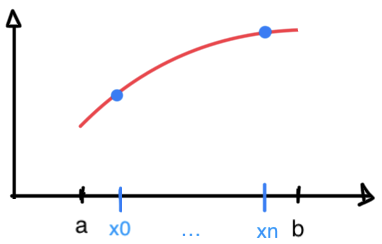
\includegraphics[width=0.5\textwidth]{immagini/GraficoAscisseInterpolazione.png}
\caption{\label{fig:GraficoAscisseInterp} Esempio delle ascisse (\ref{eq:ascisseDistinte})}
\end{figure}

\paragraph{Divagazione su $\Pi_n$:}{
$\boldsymbol{\Pi_n}$ \textbf{è lo spazio vettoriale dei polinomi di grado al più} $\boldsymbol n$. Uno spazio vettoriale è un insieme per il quale una combinazione lineare dei suoi elementi produce un elemento dello spazio stesso.
Infatti, $\forall q_1, q_2\in\Pi_n$ e $\forall \alpha,\beta\in\mathbb R$, è ottenuto che $\alpha \cdot q_1(x)+\beta\cdot q_2(x)\in\Pi_n$. $\alpha \cdot q_1(x)$ e $\beta\cdot q_2(x)$ sono moltiplicazioni che non aumentano il grado della somma, al massimo lo diminuiscono.

Se $p(x)\in\Pi_n$ è il polinomio interpolante $f(x)$, allora è possibile scriverlo come
\begin{equation}\label{eq:PolGenerico}
    p(x)=\sum_{k=0}^{n}a_kx^k.
\end{equation}
I polinomi $x^0,\, x^1,\, x^2,\, \hdots,\, x^n\in\Pi_n$ sono linearmente indipendenti e questi costituiscono la base canonica di $\Pi_n$. Pertanto, $\dim(\Pi_n)=n+1$. Questo significa che, per individuare univocamente un polinomio di $\Pi_n$,  saranno necessarie $n+1$ condizioni linearmente indipendenti.}

L'esistenza e l'unicità del polinomio interpolante è enunciata dal seguente teorema.
\begin{theorem}[Esistenza ed Unicità del polinomio interpolante]\label{th:EsisUnicPolInterp}\footnote{Slide 2 PDF 15, TH 4.1 PG 78}
    $\exists!\, p(x)\in\Pi_n: p(x_i)=f_i,\, i=0,\hdots,n$, date le coppie di dati $(x_i,f_i),\; i=0,\hdots,n$, soddisfacenti (\ref{eq:ascisseDistinte}).
\end{theorem}
\begin{proof}
    Considerato il polinomio incognito in forma (\ref{eq:PolGenerico}) ed imposte le \underline{condizioni di interpolazione (\ref{eq:condInterp})}:
    \begin{equation}\label{eq:InterpEqLin}
        p(x_i)\equiv\sum_{k=0}^{n}a_kx_i^k=f_i,\quad i=0,\hdots,n.
    \end{equation}
    Questo è un sistema di equazioni lineari $(n+1)$, nelle $n+1$ incognite $a_0,\hdots,a_n$. Il sistema può essere denotato in forma vettoriale come
    \begin{equation}\label{eq:sistemaVand}
        V\underline{a}=\underline{b},
    \end{equation}
    dove
    \begin{equation*}
        \underline{a} = 
    \begin{bmatrix}
        a_0\\
        a_1\\
        \vdots\\
        a_n
    \end{bmatrix},\; \underline{b}=
    \begin{bmatrix}
        f_0\\
        f_1\\
        \vdots\\
        f_n
    \end{bmatrix}\in\mathbb R^{n+1},\;
    V=\begin{bmatrix}
        x_0^0 & x_0^1 & \hdots & x_0^n\\
        x_1^0 & x_1^1 & \hdots & x_1^n\\
        \vdots & \vdots &\ddots & \vdots\\
        x_n^0 & x_n^1 & \hdots & x_n^n
    \end{bmatrix}\in\mathbb R^{(n+1)\times (n+1)}.
    \end{equation*}
    $V$ è la matrice dei coefficienti, definita univicomente dalle ascisse, e trasposta di una matrice di Vandermonde.

    \begin{definition}[Matrice di Vandermonde]
        Una matrice di Vandermonde ha la caratteristica di essere definita con attraverso una progressione geormetrica, ovvero gli elementi di $V$ sono del tipo $v_{i,j}=v_i^{j-1}$.
    \end{definition}
    
    \begin{remark}
        È nota la seguente proprietà delle matrici di Vandermonde, quindi di $V$: 
        \begin{equation*}
            \det(V)\overset{\footnotemark}{=}\prod_{\underbrace{i>j}_{i\neq j}}(x_i-x_j).\footnotemark
        \end{equation*}
    \end{remark}
    \footnotetext{Produttoria di tutte le coppie di elementi ascisse $x$ con indice $i>j$. Le ascisse $x_0, \hdots, x_n$ soddisfano (\ref{eq:ascisseDistinte}).}
    
    In virtù dell'ipotesi (\ref{eq:ascisseDistinte}), segue che $\det(V)\overset{\footnotemark}{\neq} 0 \Rightarrow \exists!$ la soluzione per (\ref{eq:sistemaVand}) $\iff\exists! p(x)\in\Pi_n$ che soddisfa le condizioni di interpolazione \ref{eq:condInterp}.
\end{proof}
\footnotetext{Non nullo dato che le ascisse si interpolazione $x_0, \hdots, x_n$ sono distinte.}

Il problema discreto (\ref{eq:sistemaVand}), per la determinazione di (\ref{eq:InterpEqLin}), deriva dall'aver scelto la base delle potenze, ovvero ${x^0,x^1,\hdots, x^n}$, come base di $\Pi_n$.

\begin{definition}[Polinomio Interpolante]
    Il polinomio (\ref{eq:InterpEqLin}) è noto come \textbf{polinomio interpolante} la funzione sulle ascisse assegnate.
\end{definition}

Il calcolo del polinomio interpolante tramite la risoluzione di (\ref{eq:sistemaVand}) è inefficiente per il costo computazionale elevato e per il numero di condizionamento di $V$, il quale cresce rapidamente al crescere di $n$.

È necessario cercare un modo alternativo per il calcolo del polinomio interpolante $p(x)$, ovvero utilizzare una base diversa da quella delle potenze per il polinomio interpolante. Per questo sono definiti i polinomi della seguente Sezione, atti a calcolare il polinomio interpolante con una base diversa.

\subsection{Forma di Lagrange e di Newton}
\begin{definition}[Base di Lagrange]\footnote{Slide 7 PDF 15, PG 79.}
    La \textbf{base di Lagrange} è definita dai seguenti \textbf{polinomi di Lagrange}:
    \begin{equation}\label{eq:polLagrange}
        L_{in}=\prod_{j=0,\,j\neq i}^{n} \frac{x-x_j}{x_i-x_j},\quad i=0,1,\hdots,n, 
    \end{equation}
    dove $i$ stabilisce quale polinomio è considerato ed $n$ determina il grado del polinomio.
\end{definition}

Date le ascisse definite come (\ref{eq:ascisseDistinte}), allora i polinomi di Lagrange (\ref{eq:polLagrange}) sono ben definiti ed hanno le seguenti proprietà:
\begin{itemize}
    \item[P1)] I polinomi sono ben distinti se $x_i-x_j\neq 0\,(\rightarrow x_i\neq x_j),\; i\neq j$ \footnote{Ipotesi di (\ref{eq:ascisseDistinte}).};
    \item [P2)]\footnotemark $L_{in}(x)\in\Pi_n,\; \forall i=0,\hdots,n$;
    \footnotetext{La proprietà, il grado dei polinomi $L_{in}$, non è determinata dal denominatore di $L_{in}$, ma dal nominatore di questa. $L_{in}(x)$ è una moltiplicazione di polinomi monici di grado $n$ moltiplicati $n$ volte.}
    \item[P3)]\footnote{Dimostrazione di P2).}$L_{in}(x_k)=
   \begin{cases}
     1 & \text{se $\;k=i$ (quindi nom=denom);}\\
     \underset{\footnotemark}{0} & \text{se $\;k\neq i$.}
   \end{cases}$
    \footnotetext{$x=x_j$ in almeno una moltiplicazione, quindi è 0.}
    \item[P4)] I polinomi $\{L_{0n}(x), \hdots, L_{nn}(x)\}$ sono tra loro \uline{linearmente indipendenti}\footnotemark.
    Infatti, se
    \begin{equation*}
        \sum_{i=0}^n \alpha_i\, L_{in}(x)=0, \, \forall x \Longrightarrow \alpha_i=0,\quad i=0,\hdots,n.
    \end{equation*}
    È possibile dimostrare la tesi per un generico $k\in \{0,\hdots,n\}$ valutando $0=\sum_{i=0}^n \alpha_i\, L_{in}(x_k)=\alpha_k\,\underbrace{L_{kn}(x_k)}_{1 \text{ per P3)}}=\alpha_k.$ Pertanto, $\boldsymbol{\{\underbrace{L_{0n}(x), \hdots,L_{nn}(x)}_{n+1}\}}$ costituiscono una base per $\Pi_n$, detta \textbf{base di Lagrange}.
\end{itemize}
\footnotetext{Significa che una combinazione lineare per $p$, polinomio nullo, deve essere a coefficienti nulli.}

Un'importante conseguenza dei punti P3) e P4) è il prossimo Teorema.

\begin{theorem}[Forma di Lagrange]
    Il polinomio interpolante $p(x)\in \Pi_n$, che soddisfa le condizioni (\ref{eq:condInterp}), è dato da 
    \begin{equation}\label{eq:polInterpd}
        \boldsymbol{p(x)=\sum_{k=0}^{n}} \underset{\footnotemark}{\boldsymbol{f_k}}\, \boldsymbol{L_{kn}(x)}.
    \end{equation}\footnotetext{Coefficienti di rappresentazione del polinomio interpolante rispetto alla base interpolante.}
\end{theorem}
\begin{proof}
    Definita la funzione di Kronecker (da conoscere): 
    \begin{equation}\label{eq:formaKronecker}
        L_{in}(x_i)=\delta_{ik} = 
        \begin{cases}
            \boldsymbol 1 & i=k;\\
            \boldsymbol 0 & i\neq k.
        \end{cases}
    \end{equation}
   Quindi
   \begin{equation*}
       L_{kn}(x_i)=\delta_{ki}\Rightarrow p(x_i)=\sum_{k=0}^n f_k\, L_{kn}(x_i) = \sum_{k=0}^n f_k\, \delta_{ki} = f_i \equalto{\delta_{ii}}{1} = f_i,\quad \forall i=0,\hdots,n.
   \end{equation*}
\end{proof}

\begin{definition}
    \textbf{(\ref{eq:polInterpd})} costituisce la \textbf{forma di Lagrange} del polinomio interpolante.
\end{definition}

La precedente Definizione significa che (\ref{eq:polInterpd}) è espresso rispetto alla base di Lagrange, anche se il polinomio interpolante non varia.

\begin{algorithm}
\caption{Impementazione del polinomio interpolante nella forma di Lagrange.}\label{alg:implPolIntFormaLagr}
    \begin{lstlisting}[style=Matlab-editor]
    function y = lagrange (xi, fi, x)
    %   function y = lagrange (xi, fi, x)
    %   Implementazione del polinomio interpolante nella forma di Lagrange.
    %
    %   Input:
    %   xi  - vettore delle ascisse di interpolazione (utili per calcolare f)
    %   fi  - vettore delle immagini delle xi
    %   x   - vettore delle ascisse
    %
    %   Output:
    %   y   - vettore sui dati interpolati
    %
    if length(xi) ~= length(unique(xi)), error('ascisse non distinte'), end
    if length(xi) - length(fi) ~= 0
        error('xi e fi hanno lunghezze diverse')
    end
    n = length(xi); %grado del polinomio n-1 (in Matlab i contatori sono da 1 ad n-1);
    if n < 1, error('numero di xi e fi insufficienti'), end 
    y = zeros(size(x)); %y e' una matrice quadrata con dimensione indipendente da n;
    for i = 1 : n
        y = y + fi(i) * Lin(i, xi, x);
    end
    return
    \end{lstlisting}
\end{algorithm}

\begin{algorithm}
\caption{Impementazione della base del polinomio interpolante nella forma di Lagrange.}\label{alg:implBasePolIntFormaLagr}
    \begin{lstlisting}[style=Matlab-editor]
    function L = Lin(i, xi, x)
    %
    %   function L = Lin(i, xi, x)
    %   Lin function che calcola i-esima inversa del polinomio di Lagrange.
    %   Input:
    %   i   - indice della funzione
    %   xi  - vettore ascisse sulle quali e' calcolata f
    %   x   - stesso della function lagrange
    %
    %   Output:
    %   L   - vettore con la base ricercata
    %
    %   Non sono inclusi controlli perche' svolti nel layer superiore
    L = ones(size(x));
    zi=xi(i);
    xi(i)=[];
    n = length(xi);
    for j = 1 : n
        L = L.*(x-xi(j));
    end
    L = L / prod(zi - xi);
    return
    \end{lstlisting}
\end{algorithm}

È importante utilizzare manipolazioni vettoriali al posto di cicli, in quanto le prime sono migliori per prestazioni (oltre ad essere più compatte).

Date le $n+1$ coppie $(x_i,f_i),\; i=0,\hdots,n$, con $x_i\neq x_j$, se $i\neq j$ e $f_i\overset{\footnotemark}{\equiv} f(x_i)$,
\begin{equation*}
    \boldsymbol{\exists!p(x)\in\Pi_n:p(x_i)=f_i,\quad i=0,\hdots, n},
\end{equation*}
\footnotetext{Condizione ideale perché non è sempre vero che $f$ possa essere calcolata (nel nostro lo è possibile).}
dove $p(x)$ è il polinomio interpolante di $f(x)$ sulle ascisse assegnate.

Inoltre, è utile ribadire che le rappresentazioni del polinomio interpolante (\ref{eq:PolGenerico}) e (\ref{eq:polInterpd}) sono algebricamente uguali, quindi segue che: 
\begin{equation}\label{eq:equivBasi}
p(x)=\sum_{i=0}^n \boldsymbol{a_i}\, x^i \equiv \sum_{i=0}^n f_i\, \boldsymbol{L_{in}(x)},
\end{equation}
dove $x_i$ rappresenta la base delle potenze ed $L_{in}(x)$ la base di Lagrange.

Questa semplicità formale non si concilia con requisiti computazionali per il calcolo, in modo incrementale, del polinomio.

Il problema è capire come modificare la rappresentazione del polinomio $p(x)$ rispetto alla base utilizzata, se aggiunta un'ulteriore ascissa di interpolazione $x_{n+1}\notin\{x_0,\hdots,x_n\}$, in modo da calcolare $f_{n+1}$ (ovvero $f(x_{n+1})$). Data $\widehat{p}(x)\in\Pi_{n+1}:\widehat{p}(x_i)=f_i,\, i=0,\hdots,n+1,$ è interessante capire in che relazione sono $\widehat{p}(x)$ e $p(x)$, considerando che sono considerate due basi per i polinomi. Come visto per (\ref{eq:equivBasi}), allora
\begin{equation}
    \begin{matrix}
         \widehat{p}(x)&=&\sum_{i=0}^{n+1}\boldsymbol{\widehat{a}_i}\, x^i&\equiv&\sum_{i=0}^{n+1} f_i\, \boldsymbol{L_{i,n+1}(x)},\\
        p(x)&=&\sum_{i=0}^n a_i\,\boldsymbol{x^i}&\equiv&\sum_{i=0}^n f_i\, \boldsymbol{L_{in}(x)},
    \end{matrix}
\end{equation}
con rispettivamente $\boldsymbol{\widehat{a}_i}$ ed $\boldsymbol{L_{in+1}(x)}$, $\boldsymbol{x^i}$ ed $\boldsymbol{L_{in}(x)}$ collegate fra loro.
Le funzioni di base sono le stesse, ma i coefficienti sono diversi, sono soluzione di due sistemi lineari di dimensione diversa, con matrici di coefficienti diverse (le quali non si prestano bene alla costruzione incrementale del polinomio). 

È necessario definire una base di rappresentazione, in modo tale che $\widehat p(x)$ sia ottenuta da $p(x)$, aggiungendo una funzione di base ed il relativo coefficiente, mentre tutti gli altri rimangono gli stessi di $p(x)$. Questo è possibile utilizzando, come base di rappresentazione, i \textbf{polinomi di base di Newton}:

\begin{equation}\label{eq:polBaseNewt}
    \begin{cases}
        \omega_0(x)\equiv 1;\\
        \omega_r(x)\overset{\footnotemark}{=}(x-\overset{\footnotemark}{\boldsymbol{x_{r-1}}})\,\omega_{r-1}(x),\quad r=1,\hdots,n.
    \end{cases}
\end{equation}
\addtocounter{footnote}{-1}
\footnotetext{Moltiplicazione dell'elemento $\omega_{r-1}(x)$ per un polinomio monico; $x_{r-1}$ è la $(r-1)$-esima ascissa di interpolazione.}

\stepcounter{footnote}
\footnotetext{$(r-1)$-esima ascissa di interpolazione.}

Se gli altri coefficienti delle funzioni di base rimangono gli stessi di $p(x)$ è possibile definire il nuovo polinomio ottenendo una costruzione incrementale del polinomio interpolante.

$\omega_r$ definito in (\ref{eq:polBaseNewt}) è una relazione ricorsiva utilizzata per il calcolo, in modo efficiente, di $p(x)$ e può essere rappresentato come
\begin{equation*}
    \omega_{k+1}(x)=(x-x_k)\, w_k(x),\quad k=0,\hdots, n.
\end{equation*}
oppure è possibile scriverlo come polinomio monico, ovvero il polinomio con coefficiente del termine di grado più alto uguale ad 1, in forma esplicita come
\begin{equation}\label{polBaseNewt2}
    w_k(x)=\prod_{i=0}^{k-1}(x-x_i),\quad k=1,\hdots,n.
\end{equation}

Utilizzando il principio di induzione è possibile verificare le seguenti \textbf{proprietà di} $\omega_r$:
\begin{enumerate}
    \item $w_r(x)$ è un polinomio monico di grado $r,\; \forall r\geq 0$ (ovvero $\omega_r\in\Pi_r$);
    \item $\forall r\geq 0 \, :\, \{\underbrace{\omega_0(x), \hdots, \omega_r(x)}_{r+1}\}$ sono linaremente indipendenti \footnote{Conseguenza del punto precendete dato che i gradi sono distinti.};
    \item $\{\omega_0(x),\hdots,\omega_r(x)\}$ sono una base per $\Pi_r$ \footnote{Conseguenza del punto precedente.};
    \item $\forall r \geq 1\,:\, \boldsymbol{w_r(x)=\prod_{j=0}^{r-1}(x-x_j)}$ \footnote{Ottenuta induttivamente dalla seconda riga del sistema (\ref{eq:polBaseNewt}) con gli zeri dei polinomi conosciuti. Questa relazione ricorsiva è utilizzata per il calcolo efficiente del polinomio.};
    \item Date le ascisse distinte $x_0, \hdots, x_n$:
        $\begin{cases}
        \boldsymbol{w_r(x_j)=0}, & \boldsymbol{j\leq r-1},\\
        w_r(x_j)\neq 0, & j\geq r.
        \end{cases}$
\end{enumerate}

È possibile denotare 
\begin{equation}\label{eq:polNotaz}
    p_r(x)\in\Pi_r\, :\, p_r(x_i)=f_i,\quad i=0,\hdots, r.
\end{equation}

È possibile definire la famiglia dei polinomi $\{p_r\}_{r=0,\hdots,n}$ (dove $n$ è il grado da raggiungere), in modo incrementale, con la seguente modalità.

\begin{theorem}[Forma di Newton]\label{th:formaNewt}\footnote{Slide 5 PDF 16, TH 4.3 PG 80.}
    La famiglia di polinomi interpolanti definita in (\ref{eq:polNotaz}) è ottenuta ricorsivamente come: 
    \begin{equation}\label{eq:famPolInt}
    \begin{cases}
        p_0(x)\equiv f_0\in\Pi_0\\
        p_r(x) = p_{r-1}(x)+ f[x_0,\hdots, x_r]\,\omega_r(x),\; r=1,2,\hdots
    \end{cases}
    \end{equation}
    dove $\boldsymbol{f[x_0, \hdots, x_r]}$ è la \textbf{differenza divisa di ordine $\boldsymbol r$ della funzione $\boldsymbol f$ sulle ascisse $\boldsymbol{x_0, \hdots, x_r}$}, definita come:
    \begin{equation}\label{eq:diffDivisa}
       \boldsymbol{f[x_0, \hdots, x_r] \overset{\text{def.}}{=} \sum_{i=0}^r\frac{f_i}{\prod_{j=0, j\neq i}^{r}(x_i-x_j)}}.
    \end{equation}
\end{theorem}
\begin{proof}\footnote{Dimostrazione riscorsiva del sistema (\ref{eq:famPolInt}) e di (\ref{eq:diffDivisa}).}
    Per induzione la tesi è vera, con $r=0$, poiché $p_0(x)\equiv f_0\equiv f[x_0]$. Supposto vero per $r-1$ sarà dimostrato per $r$.
    
    Per ipotesi è supposto che
    \begin{equation*}
        p_{r-1}(x)\in\Pi_{r-1}:\boldsymbol{p_{r-1}(x_i)=f_i,\; i=0,\hdots r-1}
    \end{equation*}
    e che $p(x)$ sia definto come in (\ref{eq:famPolInt}). Sarà dimostrato quanto segue:
    \begin{enumerate}
        \item $p_r(x_i)=f_i, \; i=0,\hdots,r$ \footnotemark;
        \item $f[x_0, \hdots, x_r]$ è definita come in (\ref{eq:diffDivisa}).
    \end{enumerate}
\footnotetext{Quindi è necessario dimostrare che $p_r$ è calcolabile come $p_{r-1}$.}
    \begin{proof}[Dimostrazione di 1.]
        \begin{equation*}
        \forall i=0,\hdots, r-1:\; p_r(x_i)=\underbrace{p_{r-1}(x_i)}_{f_i}+\underbrace{f[x_0, \hdots, x_r]}_{\footnotemark}\underbrace{\omega_r(x_i)}_{0}=f_i.
        \end{equation*}
        Per $i=r$, essendo le ascisse distinte, $\omega_r(x_r)\neq 0$ ed imponendo $p_r(x_r)=p_{r-1}(x_r)+f[x_0,\hdots,x_r]\,\omega_r(x_r)=f_r$ è ricavato che
        \footnotetext{Non è definito.}
        \begin{equation}\label{eq:ridefDifDivisa}
            f[x_0, \hdots, x_r]\overset{\text{def}}{=}\frac{f_r-p_{r-1}(x_r)}{\omega_r(x_r)},
        \end{equation}
        che è ben definito essendo  $\omega_r(x_r)\neq 0$.
        È necessario dimostrare che la differenza divisa espressa come (\ref{eq:ridefDifDivisa}) coincide con (\ref{eq:diffDivisa}). A questo fine è possibile osservare che $f[x_0, \hdots, x_r]$ è il coefficiente principale di $p_r(x)$.
        È definito l'algoritmo per la soluzione in due passi: 
        \begin{enumerate}
            \item scrittura di $p_r(x)$ in forma di Lagrange;
            \item calcolo del coefficiente principale di $p_r(x)$ in forma di Lagrange.
        \end{enumerate}
        Quindi i due coefficienti dovranno coincidere, per il principio di identità dei polinomi.
    
        La forma di Lagrange di $p_r(x)$ è espressa come segue:
        \begin{equation*}
            \begin{matrix}
                p_r(x) &=& \sum_{i=0}^r f_i\, \boldsymbol{L_{ir}(x)} \\
                &\overset{\footnotemark}{=}& \sum_{i=0}^r f_i\,\boldsymbol{\prod_{j=0, j\neq i}^r\frac{x-x_j}{x_i-x_j}} \\
                &=&\sum_{i=0}^r \frac{f_i}{\prod_{j=0, j\neq i}^r(x_i-x_j)}\cdot \underset{\footnotemark}{\boldsymbol{\prod_{j=0, j\neq i}^r(x-x_j)}} \\
                &\overset{\footnotemark}{=}& x^r\boldsymbol{\sum_{i=0}^r\frac{f_i}{\prod_{j=0, j\neq i}^r(x_i-x_j)}}\;+ \text{ (termini di ordine inferiore in $x$) }\\
                &\overset{\footnotemark}{\equiv}& x^r\, \boldsymbol{f[x_0,\hdots, x_r]}\; + \text{ (termini di ordine inferiore in $x$) }.
            \end{matrix}
        \end{equation*}
    \end{proof}
    \addtocounter{footnote}{-3}
    \footnotetext{Scittura del polinomio di Lagrange di grado $r$ in forma esplicita ($r\rightarrow n)$.}
    
    \stepcounter{footnote}
    \footnotetext{$\prod_{j=0,\\j\neq i}^r (x-x_j)$ è un polinomio monico di grado $r$, è una produttoria di $r$ polinomi di grado 1.}
    
    \stepcounter{footnote}
    \footnotetext{Forma di Lagrange.}
    
    \stepcounter{footnote}
    \footnotetext{Forma diversa da Lagrange.}
    Da questo è possibile concludere che la (\ref{eq:diffDivisa}) vale.

    \begin{proof}[Dimostrazione 2.]
        La seconda parte della dimostrazione del Teorema è svolta come dimostrazione del punto P5), esposto fra poco.
    \end{proof}
\end{proof}

\begin{remark}[Forma di Newton del polinomio interpolante]\label{rem:formaNewton}\footnote{Slide 8 PDF 16.}
    Sia $p(x)\in\Pi_n$, polinomio interpolante $f(x)$ sulle ascisse $\{x_0,\hdots, x_n\}$, $p(x)$ coincide con $p_n(x)$ in (\ref{eq:polNotaz}).
    Per induzione è ottenuta la \textbf{forma di Newton del polinomio interpolante}: 
    \begin{equation}\label{eq:polInterNewt}
        \boldsymbol{p(x)\equiv p_n(x) = \sum_{i=0}^{n} f[\underbrace{x_0,\hdots, x_i}_{i+1}]\,\omega_i(x)},
    \end{equation}
    dove $\omega_i(x)$ è la dunzione di base.
\end{remark}

\paragraph{\ul{N.B.}:} \textbf{La forma di Lagrange e la forma di Newton di $p(x)$ definiscono lo stesso polinomio interpolante}, il quale esiste ed è unico, se le ascisse di interpolazione sono tra loro distinte. Ciò significa che per $p(x)$ varia solo la sua rappresentazione. Questo ha il pregio di prestarsi alla costruzione incrementale del polinomio aggiornandosi in modo dinamico.

\paragraph{Esempio di caso d'uso polinomio interpolante:} se fosse richiesto di approssimare ciò che è sotto una certa curva questa viene calcolata con un numero prefissato di punti, poi se ne sono aggiungono uno ad uno fino a che non è più possibile effetturare una stima accurata.

La definizione in forma di Newton di $p(x)$ come (\ref{eq:polInterNewt}) permette di ottenere funzioni di base in funzione delle precedenti. Pertanto, questo non permette di calcolare la differenza divisa e la rappresentazione $f[x_0,\hdots, x_r]$ non è algoritmicamente preferibile. Per arrivare al fine di ottenere un algoritmo efficiente, sono esaminate alcune proprietà delle differenze divise.

\paragraph{\underline{Proprietà differenze divise (\ref{eq:diffDivisa})}:} \footnote{Slide 9-11 PDF 16, TH 4.4 PG 82.}
\begin{itemize}
    \item[P1)](Linearità dell'operatore) Se $f$ e $g$ sono funzioni in variabili reali $\alpha,\,\beta \in\mathbb R$, allora
    \begin{equation*}
        (\alpha\cdot f + \beta\cdot g)[x_0,\hdots, x_r]=\alpha\cdot f[x_0,\hdots, x_r]+\beta\cdot g[x_0,\hdots, x_r];
    \end{equation*}
    \item[P2)](Simmetria dell'operatore) Se $\{i_0,\hdots,i_r\}$ è una permutazione di $\{0,\hdots, r\}$, allora:
    \begin{equation*}
        f[x_0,\hdots,x_r]=f[x_{i_0},\hdots,x_{i_r}];
    \end{equation*}
    \item[P3)] Se $f(x)=\sum_{i=0}^ka_ix^i$, allora $f[x_0,\hdots, x_r]=
    \begin{cases}
        a_k,\; r=k;\\
        0,\; r>k.
    \end{cases}$
    \footnote{Sia $g(x)\in\Pi_n$, allora il polinomio $p(x)\in\Pi_n$ che interpola $g(x)$ sulle ascisse distinte $x_0,\hdots,x_n$ è $g(x)$ stesso ($p(x)=g(x)$), per l'unicità del polinomio interpolante.
    Il polinomio $p(x)\in\Pi_r,$ con $r>n$, che interpola $g(x)$ sulle $r+1$ ascisse distinte $x_0, \hdots, x_r$, è sempre $g(x)$ per lo stesso motivo.}

    \item[P4)] Se $f\in C^{(\boldsymbol r)}[a,b],\, a=\underset{i=0,\hdots,\boldsymbol r}{\min}x_i,\, b=\underset{i=0,\hdots,\boldsymbol r}{\max}x_0$, allora
    \begin{equation}\label{eq:P4DiffDiv}
        f[x_0,\hdots, x_{\boldsymbol r}]=\frac{f^{(\boldsymbol r)}(\xi)}{\boldsymbol r!},\; \xi\in [a,b],
    \end{equation}

    dove $[a,b]$ è il più piccolo intervallo che contiene le ascisse di interpolazione. Questa proprietà vale anche nel caso in cui 2 o più ascisse coincidano. In questo caso, la definizione di differenza divisa vale come limite.

    \item[P5)] \begin{equation}\label{eq:P5DiffDiv}
        f[\underbrace{x_0,\hdots,x_r}_{r+1}]=\frac{f[\overbrace{x_1,\hdots,x_r}^{r}]-f[\overbrace{x_0,\hdots,x_{r-1}}^{r}]}{x_r-x_0}.\footnotemark
    \end{equation}
    \footnotetext{Le due differenze divise al nominatore differiscono solo per l'ascissa $x_0$. Il concetto è che, se è applicata iterativamente questa proprietà, allora è possibile scrivere le differenze divise come combinazione di differenze divise, con $r-1$ argomenti, fino ad ottenere un solo argomento. Quando l'argomento è unico allora la differenza divisa coinciderà con il valore calcolato nell'argomento.}
\end{itemize}

(\ref{eq:P5DiffDiv}) è  una proprietà algoritmica importante, è utilizzata per il calcolo efficiente della differenze divisa ed è possibile dimostrarla come segue.

\begin{proof}[Dimostrazione P5)] \footnote{Tramite la definizione di differenza divisa. Sono calcolate due differenze divise, è effettuata la somma ed è ottenuta l'espressione ricercata.}
    \begin{equation}\label{eq:dimPropDiffDiv}
        \begin{matrix}
            \frac{1}{x_r-x_0}(f[x_1,\hdots, x_r]-f[x_0,\hdots,x_{r-1}]) = \frac{1}{x_r-x_0}\left(\sum_{k=1}^r\frac{f_k}{\prod_{j=1,j\neq k}^r(x_k-x_j)}-\sum_{k=0}^{r-1}\frac{f_k}{\prod_{j=0,j\neq k}^{r-1}(x_k-x_j)}\right)\\
            = \frac{1}{x_r-x_0}\,\left(\underbrace{\overbrace{\frac{f_r}{\prod_{j=1,j\neq r}^r(x_r-x_j)}}^{(a)}-\overbrace{\frac{f_0}{\prod_{j=0,j\neq 0\rightarrow j=1}^{r-1}(x_0-x_j)}}^{(b)}}_{\text{Elementi comuni alle due sommatorie}}+\underbrace{\sum_{k=1}^{r-1}f_k\,\left(\frac{1}{\prod_{j=1,j\neq k}^r(x_k-x_j)}-\frac{1}{\prod_{j=0,j\neq k}^{r-1}(x_k-x_j)}\right)}_{\underset{\footnotemark}{(c)}}\right)\\
             =(a)+(b)+(c),
        \end{matrix}
    \end{equation}
    \footnotetext{Dato che gli indici da 1 ad $r-1$ sono comuni ad entrambe le produttorie, saranno raggruppati gli addendi con indici comuni e lasciati gli addendi non comuni. Addendi con indice uguale ad $r$ sono sommatorie, con indice uguale a 0 sono la somma $a+b$.}
    dove $\frac{1}{x_r-x_0}$ è inglobata in $(a),(b)$ e $(c)$ come segue:
    \begin{equation*} 
        \begin{matrix}
        (a) = \frac{1}{x_r-x_0}\frac{f_r}{\prod_{j=1,j\neq r}^r(x_r-x_j)}\overset{\footnotemark}{=}\frac{f_r}{\prod_{j=0,j\neq r}^r(x_r-x_j)};\\
        (b) = \frac{1}{x_0-x_r}=\frac{f_0}{\prod_{j=0,j\neq 0}^{r-1}(x_0-x_j)}=\frac{f_0}{\prod_{j=0,j\neq 0}^r(x_0-x_j)};\\
        (c) = \frac{1}{x_r-x_0}\sum_{k=1}^{r-1}\frac{f_k}{\prod_{j=1,j\neq k}^{r-1}(x_k-x_j)}\underbrace{\left(\frac{1}{x_k-x_r}-\frac{1}{x_k-x_0}\right)}_{\footnotemark}=
        \frac{1}{\cancel{x_r-x_0}}\sum_{k=1}^{r-1}\frac{f_k}{\prod_{j=1,j\neq k}^{r-1}(x_k-x_j)}\left(\frac{\cancel{x_k}-\cancel{x_0}-\cancel{x_k}+\cancel{x_r}}{(x_k-x_r)(x_k-x_0)}\right)=\\
        \sum_{k=1}^{r-1}\frac{f_k}{\prod_{j=0,j\neq k}^{r-1}(x_k-x_j)};
        \end{matrix}
    \end{equation*}
    \addtocounter{footnote}{-1}
    \footnotetext{Ultimo termine della sommatoria della differenza divisa delle ascisse $x_0,\hdots,x_r$.}
    \stepcounter{footnote}
    \footnotetext{Termini necessari per le caratteristiche degli indici.}
    
    Pertanto, unendo i precedenti risultati:
    \begin{equation*}
        \textbf{(\ref{eq:dimPropDiffDiv})}=\sum_{k=0}^r\frac{f_k}{\prod_{j=0,j\neq k}^r (x_k-x_j)}\overset{\footnotemark}{=} f[x_0,x_1,\hdots,x_r].
    \end{equation*}
    \footnotetext{Ovvero ciò che è necessario dimostrare.}
\end{proof}

\paragraph{Esempio di utilizzo della proprietà (\ref{eq:P5DiffDiv}):} Considerando il caso $\boldsymbol{n=3}$:
\begin{equation*}
    \boldsymbol{p(x)=f[x_0]\;\equalto{\omega_0(x)}{1}+f[x_0,x_1]\omega_1(x)+f[x_0,x_1,x_2]\omega_2(x)+f[x_0,x_1,x_2,x_3]\omega_3(x)},
\end{equation*}
allora è possibile generalizzarlo in la seguente tabella triangolare:
 
\begin{center}
\begin{tabular}{|c|c|c|c|c|} 
\hline
 & $\overset{\footnotemark}{0}$ & $\overset{\footnotemark}{1}$ & 2 & 3 \\
\hline
$x_0$ & $\boldsymbol{f_0 = f[x_0]}$ & & &  \\ 
$x_1$ & $f_1 = f[x_1]$ & $\boldsymbol{f[x_0,x_1]}$ & &  \\ 
$x_2$ & $f_2 = f[x_2]$ & $f[x_1,x_2]$ &$ \boldsymbol{f[x_0,x_1,x_2]}$ & \\
$x_3$ & $f_3 = f[x_3]$ & $f[x_2, x_3]$ & $f[x_1,x_2,x_3]$ & $\boldsymbol{f[x_0,x_1,x_2,x_3]}$ \\
\hline
\end{tabular}
\end{center}
\addtocounter{footnote}{-1}
\footnotetext{Differenza tra l'indice delle ascisse (utillizzata la proprietà incementale delle differenze divise).}

\stepcounter{footnote}
\footnotetext{Differenze divise su due ascisse.}

Gli elementi sulla diagonale principale, ovvero quelli in grassetto, sono i coefficienti del polinomio interpolante nella forma di Newton (\ref{eq:polInterNewt}).

La tabella è calcolata dal basso verso l'alto per evitare di memorizzare tutti i dati della tabella. Non è necessario memorizzarla tutta perché è possibile sovrascrivere gli elementi a sinistra con quelli a destra (quindi in fine saranno presenti le differenze divise in grassetto). Per questo è necessario calcolare prima la colonna 0 e poi la 1, 2 e 3 sovrascrivendone, via via, gli elementi. Quanto appena scritto non è valido se gli elementi sono calcolati dall'alto verso il basso.

Utilizzando il metodo di calcolo più conveniente è possibile utilizzare due vettori: uno per le ascisse di interpolazione $(x_0,\hdots, x_3)$ ed uno per i dati del problema da sovrascrivere con i coefficienti dei polinomi.

La tabella ha complessità quadratica, come la forma di Lagrange, e minore rispetto a risolvere il sistema lineare con la matrice di Vandermonde (la quale ha complessità $\frac{2}{3}n^3$).

Le colonne della precedente tabella, dalla 1 alla 3, sono determinate (calcolate) dal basso verso l'alto come segue:

\begin{equation*}
    \begin{matrix}
        \underset{\footnotemark}{\boldsymbol 1}
    \begin{cases}
        f[x_2,x_3]=\frac{f[x_3]-f[x_2]}{x_{\boldsymbol 3}-x_{\boldsymbol 2}}\\
        f[x_1,x_2]=\frac{f[x_2]-f[x_1]}{x_{\boldsymbol 2}-x_{\boldsymbol 1}}\\
        f[x_0,x_1]=\frac{f[x_1]-f[x_0]}{x_{\boldsymbol 1}-x_{\boldsymbol 0}}
    \end{cases}\\
    \boldsymbol{2}\begin{cases}
        f[x_1,x_2,x_3]=\frac{f[x_{\boldsymbol 2},x_3]-f[x_1,x_{\boldsymbol 2}]}{x_{\boldsymbol 3}-x_{\boldsymbol 1}}\\
        f[x_0,x_1,x_2]=\frac{f[x_{\boldsymbol 1},x_2]-f[x_0,x_{\boldsymbol 1}]}{x_{\boldsymbol 2}-x_{\boldsymbol 0}}
    \end{cases}\\
    \boldsymbol{3}\begin{cases}
        f[x_0,x_1,x_2,x_3]=\frac{f[\boldsymbol{x_1,x_2},x_3]-f[x_0,\boldsymbol{x_1,x_2}]}{x_{\boldsymbol 3}-x_{\boldsymbol 0}}
    \end{cases}
    \end{matrix}
\end{equation*}
\footnotetext{Differiscono di un'ascissa non comune.}

È possibile notare che al denominatore le ascisse di iterpolazione differiscono rispettivamente, dall'alto al basso, di un indice 1, 2 e 3 e che tali ascisse non sono comuni alle differenze divise al denominatore delle rispettive frazioni.

\begin{remark}\footnote{Slide 6 PDF 17.}
    Nel caso generale, la precedente tabella arriverà fino a colonna $n$ (l'indice partirà da 0) ed avrà struttura analoga.
\end{remark}

\begin{algorithm}
\caption{Calcolo delle differenze divise.}\label{alg:calcDiffDiv}
    \begin{lstlisting}[style=Matlab-editor]
        % x - ascisse di interpolazione
        % f - valori della funzione nelle ascisse
        % x ed f sono vettori di dimensione n+1 perche' Matlab utilizza indici che partono da 1
        n = length(x)-1; % grado del polinomio
        for j = 1 : n
            for i = n+1 : -1 : j+1
                f(i)=(f(i)-f(i-1))/(x(i)-x(i-j)); %saranno modificati in colonna j gli elementi che vanno dall'ultimo al j+1-esimo. Il j-esimo contiente la differenza divisa, la quale e' calcolata nella riga della nota
            end
        end
    \end{lstlisting}
\end{algorithm}

\begin{remark} Il \textbf{costo computazionale} dell'\textbf{Algoritmo (\ref{alg:calcDiffDiv}}) è
    \begin{itemize}
        \item $\sum_{j=1}^{n}3(n-j+1)\overset{\footnotemark}{=} 3\sum_{j=1}^{n}j=3\cdot\frac{n(n+1)}{2}\boldsymbol{\approx \frac{3}{2}n^2\; flops}$; \footnotetext{Somma naturale.}
        \item \textbf{2 vettori} $\boldsymbol{(x, f)}$ ($x$ memorizza le ascisse interpolanti ed $f$ le differenze divise);
    \end{itemize}
\end{remark}

\noindent\textbf{Problema:} È necessario considerare il calcolo efficiente del polinomio di Newton. Del polinomio sono noti i coefficienti ed è necessario calcolare la sommatoria. Sarà utilizzata la proprietà ricorsiva del polinomio di Newton. Al fine del calcolo efficiente del polinomio di Newton è valutato un problema più semplice rispetto alla base delle potenze, il calcolo del polinomio (\ref{eq:PolGenerico})  $\left(p(x)=\sum_{k=0}^{n}a_kx^k\right)$.

Partendo da un caso semplice, ovvero con $n=3$:
\begin{equation*}
    p(x)=a_0+a_1\,x+a_2\,x^2+a_3\,x^3\overset{\footnotemark}{=} a_0+ x(a_1+x(a_2+x\,a_3)).
\end{equation*}\footnotetext{Raggruppamento.}

Supposto di avere il vettore $a=[\underbrace{\overbrace{a_0\; a_1\; \hdots\; a_n}^{n+1\text{ elementi}}}_{\footnotemark}]$ \footnotetext{In Matlab è necessario rappresentarli come $a(1)\; a(2)\,\hdots\, a(n+1)$.} è possibile calcolare il polinomio tramite l'Algoritmo \ref{alg:polHorn}.

\begin{algorithm}
\caption{Algoritmo di Horner per il calcolo di un polinomio.}\label{alg:polHorn}
    \begin{lstlisting}[style=Matlab-editor]
        p = a(n+1); % al termine dell'algoritmo conterra' il valore del polinomio
        for i = n : -1 : 1
            p = p .* x + a(i);
        end
    \end{lstlisting}
\end{algorithm}

\begin{remark}[Costo dell'Algoritmo \ref{alg:polHorn}]
    Il costo dell'algoritmo è $2n\, flops$ (\underline{per componente di $x$}).
\end{remark}

L'Algoritmo \ref{alg:polHorn} (di Horner) ha un costo minimale: sono svolte due operazioni algebriche elementari per calcolare il vettore $p(x)$, per iterazione. È, inoltre, importante osservare che questo algoritmo si presta ad essere vettorizzato in Matlab, attraverso la moltiplicazione vettoriale .*, dove $x$, in riga 3 dell'Algoritmo \ref{alg:polHorn}, può essere di qualsivolglia forma (vettore, elemento singolo, matrice). Utilizzare le capacità vettoriali di Matlab rende più efficiente il codice (quindi è necessario utilizzarlo nell'elaborato).

Inoltre, è possibile generalizzare la differenza divisa al caso della base di Newton attraverso l'algoritmo di Horner generalizzato (Algoritmo \ref{alg:polHornMod}).

\begin{example}
    Con $n=3$:
    \begin{equation*}
        \begin{matrix}
            p(x) &\overset{\footnotemark}{=}& f[x_0] + f[x_0,x_1]\,\omega_1(x) + f[x_0,x_1,x_2]\,\omega_2(x) + f[x_0,x_1,x_2,x_3]\,\omega_3(x)\\
            &\overset{\footnotemark}{=}& f[x_0]+f[x_0,x_1](x-x_0)+f[x_0,x_1,x_2](x-x_0)(x-x_1)+f[x_0,x_1,x_2,x_3](x-x_0)(x-x_1)(x-x_2)\\
            &=&\left(\left(f[x_0,x_1,x_2,x_3](x-x_2) + f[x_0,x_1,x_2]\right)(x-x_1)+f[x_0,x_1]\right)(x-x_0)+f[x_0].
        \end{matrix}
    \end{equation*}
    \addtocounter{footnote}{-1}
    \footnotetext{È noto come calcolare le defferenze divise (ovvero i coefficienti).}
    \stepcounter{footnote}
    \footnotetext{Scrittura di $\omega_i(x)$ (polinomio di Newton) in forma estesa in modo da appurare efficientemente il valore in un punto, o in più di uno. La forma estesa è la forma in cui i polinomi in base di Newton sono usati perché la loro espressione è nota.}
\end{example}

\begin{algorithm}
\caption{Algoritmo di Horner generalizzato (per il calcolo di un polinomio).}\label{alg:polHornMod}
    \begin{lstlisting}[style=Matlab-editor]
        % f(1), ..., f(n+1)   - calcolato dal codice precedente per le differenze divise
        % x(1), ..., x(n+1)   - contiene le ascisse di interpolazione
        p = f(n+1) 
        for i = n : -1 : 1
            p = p .* (x - x(i)) + f(i)
        end
    \end{lstlisting}
\end{algorithm}

\begin{remark}
    L'operazione .* in riga 5 dell'Algoritmo \ref{alg:polHornMod} è vettorizzabile.
\end{remark}

\begin{remark}[Costo dell'Algoritmo \ref{alg:polHornMod}]
    Il costo dell'algoritmo è $3n$ flops per componente.
\end{remark}

\paragraph{Intermezzo per la definizione della "Interpolazione di Hermite"}\footnote{Slides 1-3 PDF 18.} Dato il polinomio interpolante in forma di Newton (\ref{eq:polInterNewt}) allora è possibile utilizzare l'Algoritmo \ref{alg:calcP(x)} per calcolare $p(x)$.

\begin{algorithm}\caption{Pseudo-codice calcolo $p(x)$.}\label{alg:calcP(x)}
    \begin{algorithmic}
        \State $w_0\equiv 1$
        \State $p = 0$
        \For{i = 0 : n}
            \State $p = p + \omega_i * a_i$
            \State $\omega_{i+1} = \omega_i *(x - x_i)$
        \EndFor
    \end{algorithmic}
\end{algorithm}

L'Algoritmo \ref{alg:calcP(x)} utilizza il fatto che le funzioni di base possano essere ottenute in modo iterativo, moltiplicando un termine di grado uno (il polinomio monico). Pertanto, è meno efficiente dell'Algoritmo (di Horner generalizzato) \ref{alg:polHornMod} in quanto effettua $4n\, flops$ ed utilizza una variabile di appoggio ($\omega$, la quale rappresenta $\omega_0,\,\omega_1,\,\omega_{i+1}$).

Tuttavia, l'Algoritmo \ref{alg:calcP(x)} si presta facilmente per derivare un algoritmo per il calcolo della derivata prima di $p(x)$, la quale sarà significativa per gli argomenti che saranno trattati, ovvero:
\begin{equation*}
    \boldsymbol{p'(x)}=\sum_{i=0}^n\underset{\text{coeff.}}{a_i}\,\boldsymbol{\omega'_i(x)}=\sum_{\underset{\footnotemark}{i=1}}^na_i\,\boldsymbol{\omega'_i(x)}.
\end{equation*}
\footnotetext{Trasformazione in $i=1$ perché $\omega_0\equiv 1$ (vedere (\ref{eq:polBaseNewt})).}

L'obbiettivo è derivare un algoritmo per il calcolo delle derivate $\omega'(x)$ e $p'(x)$. Ciò significa che le righe precedenti si riducono a derivare un algoritmo, relativamente efficiente, per il calcolo delle derivate prime dei polinomi di base di Newton.

È possibile osservare che il calcolo di $\omega_i(x)$ come
\begin{equation*}
    \omega_i(x)=\prod_{k=0}^{i-1}(x-x_k)\Rightarrow \omega'_i(x)=\sum_{k=0}^{i-1}\prod_{j=0,j\neq k}^{i-1}(x-x_j)
\end{equation*}
è dispendioso e poco efficiente, se calcolato in questo modo.

\begin{example}
    $\omega_2(x)=(x-x_0)(x-x_1) \rightarrow \omega'_2(x)=(x-x_0)+(x-x_1)$.
\end{example}

\begin{remark}
    È possibile ottenere i polinomi, in modo ricorsivo, dall'Algoritmo \ref{alg:calcP'(x)} (ultima riga del for), ovvero:
    \begin{equation*}
        \begin{cases}
            \omega_0(x)\equiv 1,\, \omega'_0(x)\equiv 0,\\
            i\geq 1\,:\, \omega'_i(x)=\frac{\partial f}{\partial x}[\omega_{i-1}(x)(x-x_{i-1})] = \omega'_{i-1}(x)(x-x_{i-1})+\omega_{i-1}(x).
        \end{cases}
    \end{equation*}
\end{remark}

Questa osservazione porta alla definizione dell'Algoritmo \ref{alg:calcP'(x)} (dove $\omega_i$ rimane una variabile). L'algoritmo utilizza una variabile per la derivata, $\omega'_i$, ed una per il polinomio di base, $p'_i$. Pertanto, dato un polinomio, espresso con base di Newton, è noto come calcolarlo e con esso la sua derivata prima.

\begin{algorithm}\caption{Algoritmo calcolo $p'(x)$.}\label{alg:calcP'(x)}
    \begin{algorithmic}
        \State $w_0=1,\, \omega'_0=0,\, p'=0$
        \For{$i=1:n$}
            \State $\omega'_i=\omega'_{i-1}+\omega'_{i-1}\cdot (x-x_{i-1})$
            \State $\omega_i=\omega_{i-1}\cdot(x-x_{i-1})$
            \State $p'=p'+a_i\cdot\omega'_i$
        \EndFor
    \end{algorithmic}
\end{algorithm}

\subsection{Interpolazione di Hermite}\footnote{Slide 4-11 PDF 18, PG 84-86.}
[Problema:] Supposto di avere un polinomio interpolante una funzione su un numero pari ($2n+2$) di ascisse, quest'ultime sono numerate come segue:
\begin{equation}
    a\leq\overbrace{x_0 < x_{\frac{1}{2}} < x_1 < x_{\frac{3}{2}} < \hdots < x_n < x_{n+\frac{1}{2}}}^{2n+2\text{ ascisse}}\leq b.
\end{equation}

Pertanto, sotto la precedente ipotesi di ascisse distinte, $\boldsymbol{\exists!\, p(x)}\in\Pi_{\boldsymbol{2n+1}}$ (condizione importante) tale che le condizioni del polinomio interpolante (\ref{eq:condInterp}) diventano le seguenti:
\begin{equation}\label{eq:hermCondPolInterp}
    \begin{rcases}
        \boldsymbol{p(x_i)=f(x_i)}\\
        \boxed{p\left(x_{i+\frac{1}{2}}\right)=f\left(x_{i+\frac{1}{2}}\right)}
    \end{rcases} i=0,\hdots,n.
\end{equation}

Se $\forall i=0,\hdots,n: x_{i+\frac{1}{2}}\rightarrow x_i$, le ascisse che sono tra due interi, quelle con indice frazionario (ovvero $i+\frac{1}{2}$), sono fatte tendere all'ascissa a sinistra, quindi la condizione di interpolazione è duplicata. Per evitare la duplicazione è possibile riscrivere le condizioni di interpolazione (\ref{eq:hermCondPolInterp}), in modo equivalente, come:
\begin{equation}\label{eq:hermCondPolInterpMod}
    \begin{rcases}
        \boldsymbol{p(x_i)=f(x_i})\\
        \boxed{\frac{p\left(x_{i+\frac{1}{2}}\right)-p(x_i)}{x_{i+\frac{1}{2}}-x_i}=\frac{f\left(x_{i+\frac{1}{2}}\right)-f(x_i)}{x_{i+\frac{1}{2}}-x_i}}
     \end{rcases} i=0,\hdots,n,
\end{equation}
per
\begin{equation*}
    x_{i+\frac{1}{2}}\rightarrow x_i:
    \begin{cases}
        \frac{p\left(x_{i+\frac{1}{2}}\right)-p(x_i)}{x_{i+\frac{1}{2}}-x_i}\rightarrow p'(x_i)\\
        & i=0,\hdots, n.\\
        \frac{f\left(x_{i+\frac{1}{2}}\right)-f(x_i)}{x_{i+\frac{1}{2}}-x_i}\rightarrow f'(x_i)
    \end{cases}
\end{equation*}

\begin{remark}
    La seconda condizione di (\ref{eq:hermCondPolInterp}) è stata modificata nella seconda condizione di (\ref{eq:hermCondPolInterpMod}), sottraendo la prima condizione alla seconda di (\ref{eq:hermCondPolInterp}) e dividendo membro a membro per $x_{i+\frac{1}{2}}-x_i$.
\end{remark}

Data $f(x)\in C^{(1)}$ è possibile ottenere ciò che segue (vedere (\ref{eq:P4DiffDiv})):
\begin{equation}\label{eq:equivApproxf'}
    \frac{f\left(x_{i+\frac{1}{2}}\right)-f(x_i)}{x_{i+\frac{1}{2}}-x_i}=f\left[x_i,x_{i+\frac{1}{2}}\right]\rightarrow f[x_i,x_i]\equiv f'(x_i),\; i=0,\hdots,n.
\end{equation}

È possibile concludere che se $x_{i+\frac{1}{2}}\rightarrow x_i,\, \forall i=\underbrace{0,\hdots, n}_{\footnotemark}\Rightarrow\exists! p_{\boldsymbol H}(x)\in\Pi_{\boldsymbol{2n+1}}$ tale che: \footnotetext{Quindi le ascisse sono $n+1$.}
\begin{equation}\label{eq:polInterHer}
    \footnotemark\begin{cases}
        p_{\boldsymbol H}(x_i)=f(x_i)\\
        p_{\boldsymbol H}'(x_i)=f'(x_i)
    \end{cases} i=\boldsymbol{0,\hdots,n}.
\end{equation}\footnotetext{Condizioni su polinomio e sulla sua derivata prima.}

\begin{definition}[Polinomio interpolante di Hermite]
    $p_{\boldsymbol H}(x)$ è il polinomio interpolante di Hermite.  
\end{definition}

Pertanto, date le $n+1$ ascisse distinte (\ref{eq:ascisseDistinte}), $\exists!\, p_{\boldsymbol H}(x)\in\Pi_{2n+1}$, che soddisa le condizioni di interpolazione (\ref{eq:polInterHer}). Il polinomio $p_H(x)$ interpola la funzione $f(x)$ e la sua derivata, $f'(x)$, nelle ascisse di interpolazione.

\begin{example}\footnote{Slide 5 PDF 18.}
    Considerate le ascisse $x_i=i\cdot\pi,\; i=0,1,2$ e considerando la funzione
    \begin{equation*}
        f(x)=\sin(x)\overset{\footnotemark}{\Rightarrow}f'(x)=\cos(x).
    \end{equation*}
    Spiegazione grafica dell'esempio in Figura \ref{fig:PolHermite} e \ref{fig:PolHermite1}. \footnotetext{Il polinomio interpolante classico è il polinomio costante 0 perché interpola $f(x)$ nelle 3 ascisse di interpolazione. Il polinomio di Hermite interpola anche la deriva prima, ciò rende l'approssimazione più accurata rispetto a quella del polinomio classico.}
\end{example}

\begin{figure}
\centering
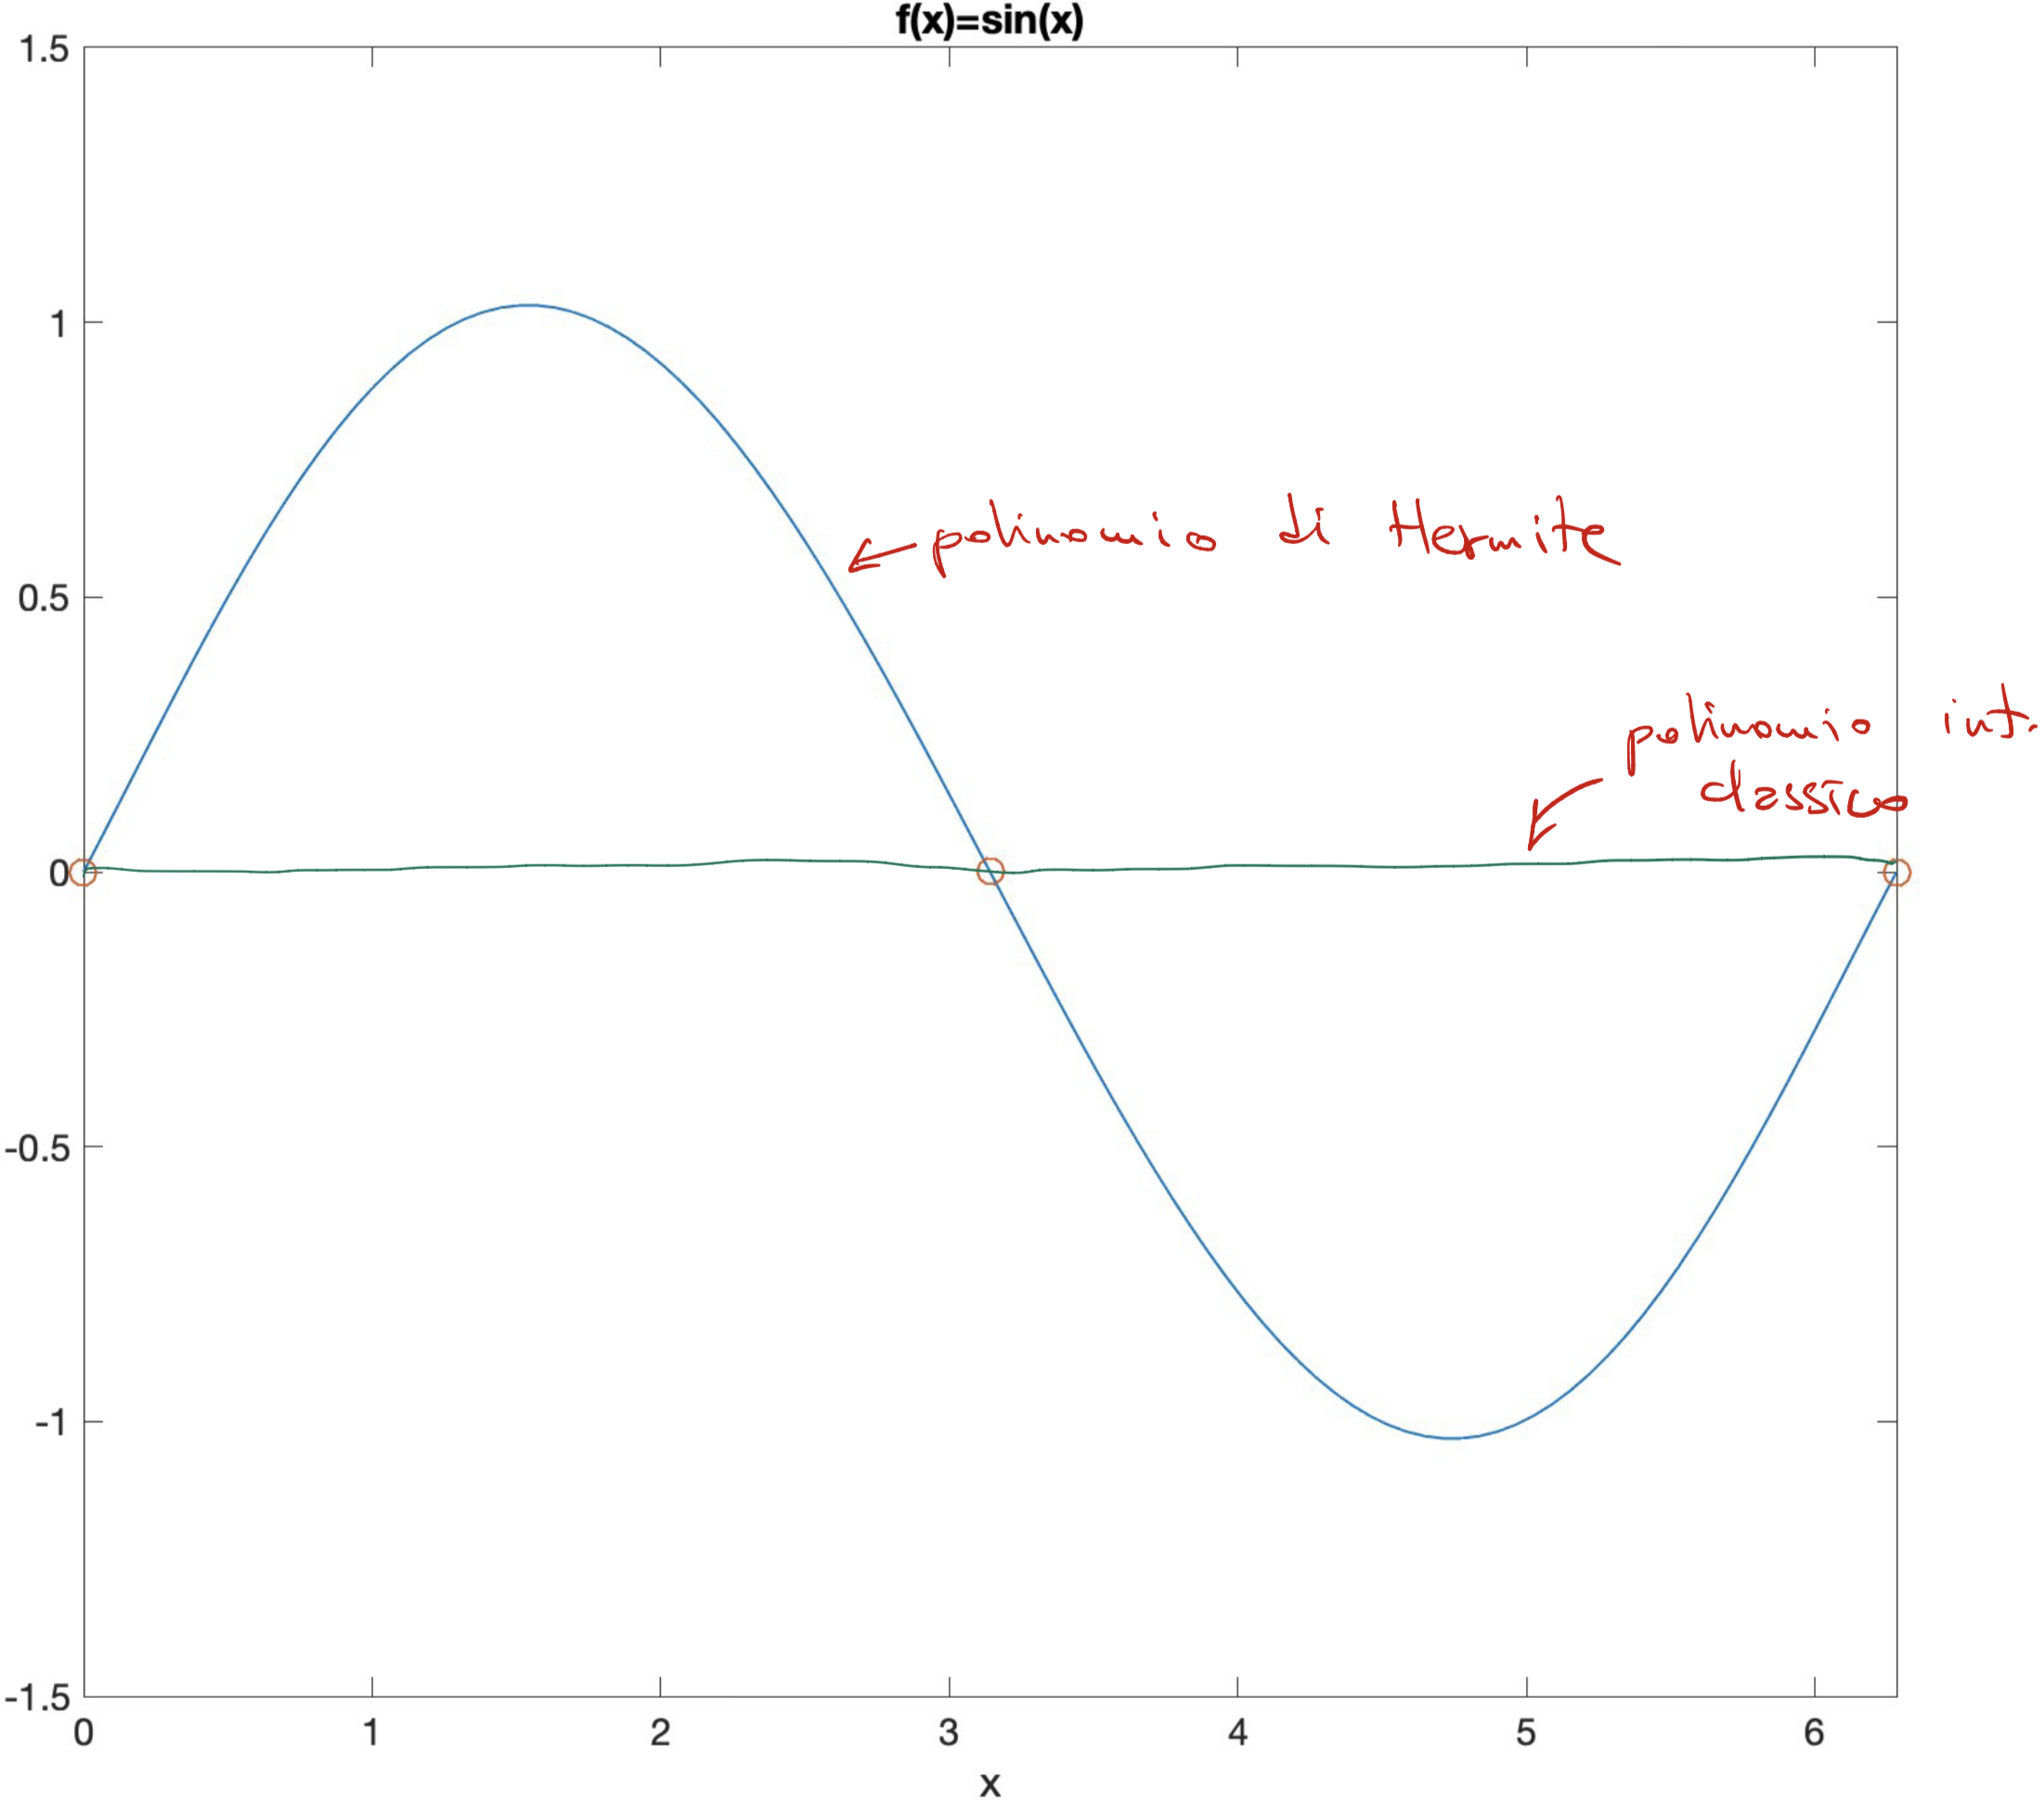
\includegraphics[width=0.5\textwidth]{immagini/PolHermite.png}
\caption{\label{fig:PolHermite} Esempio delle differenze di approssimazione}
\end{figure}
\begin{figure}
\centering
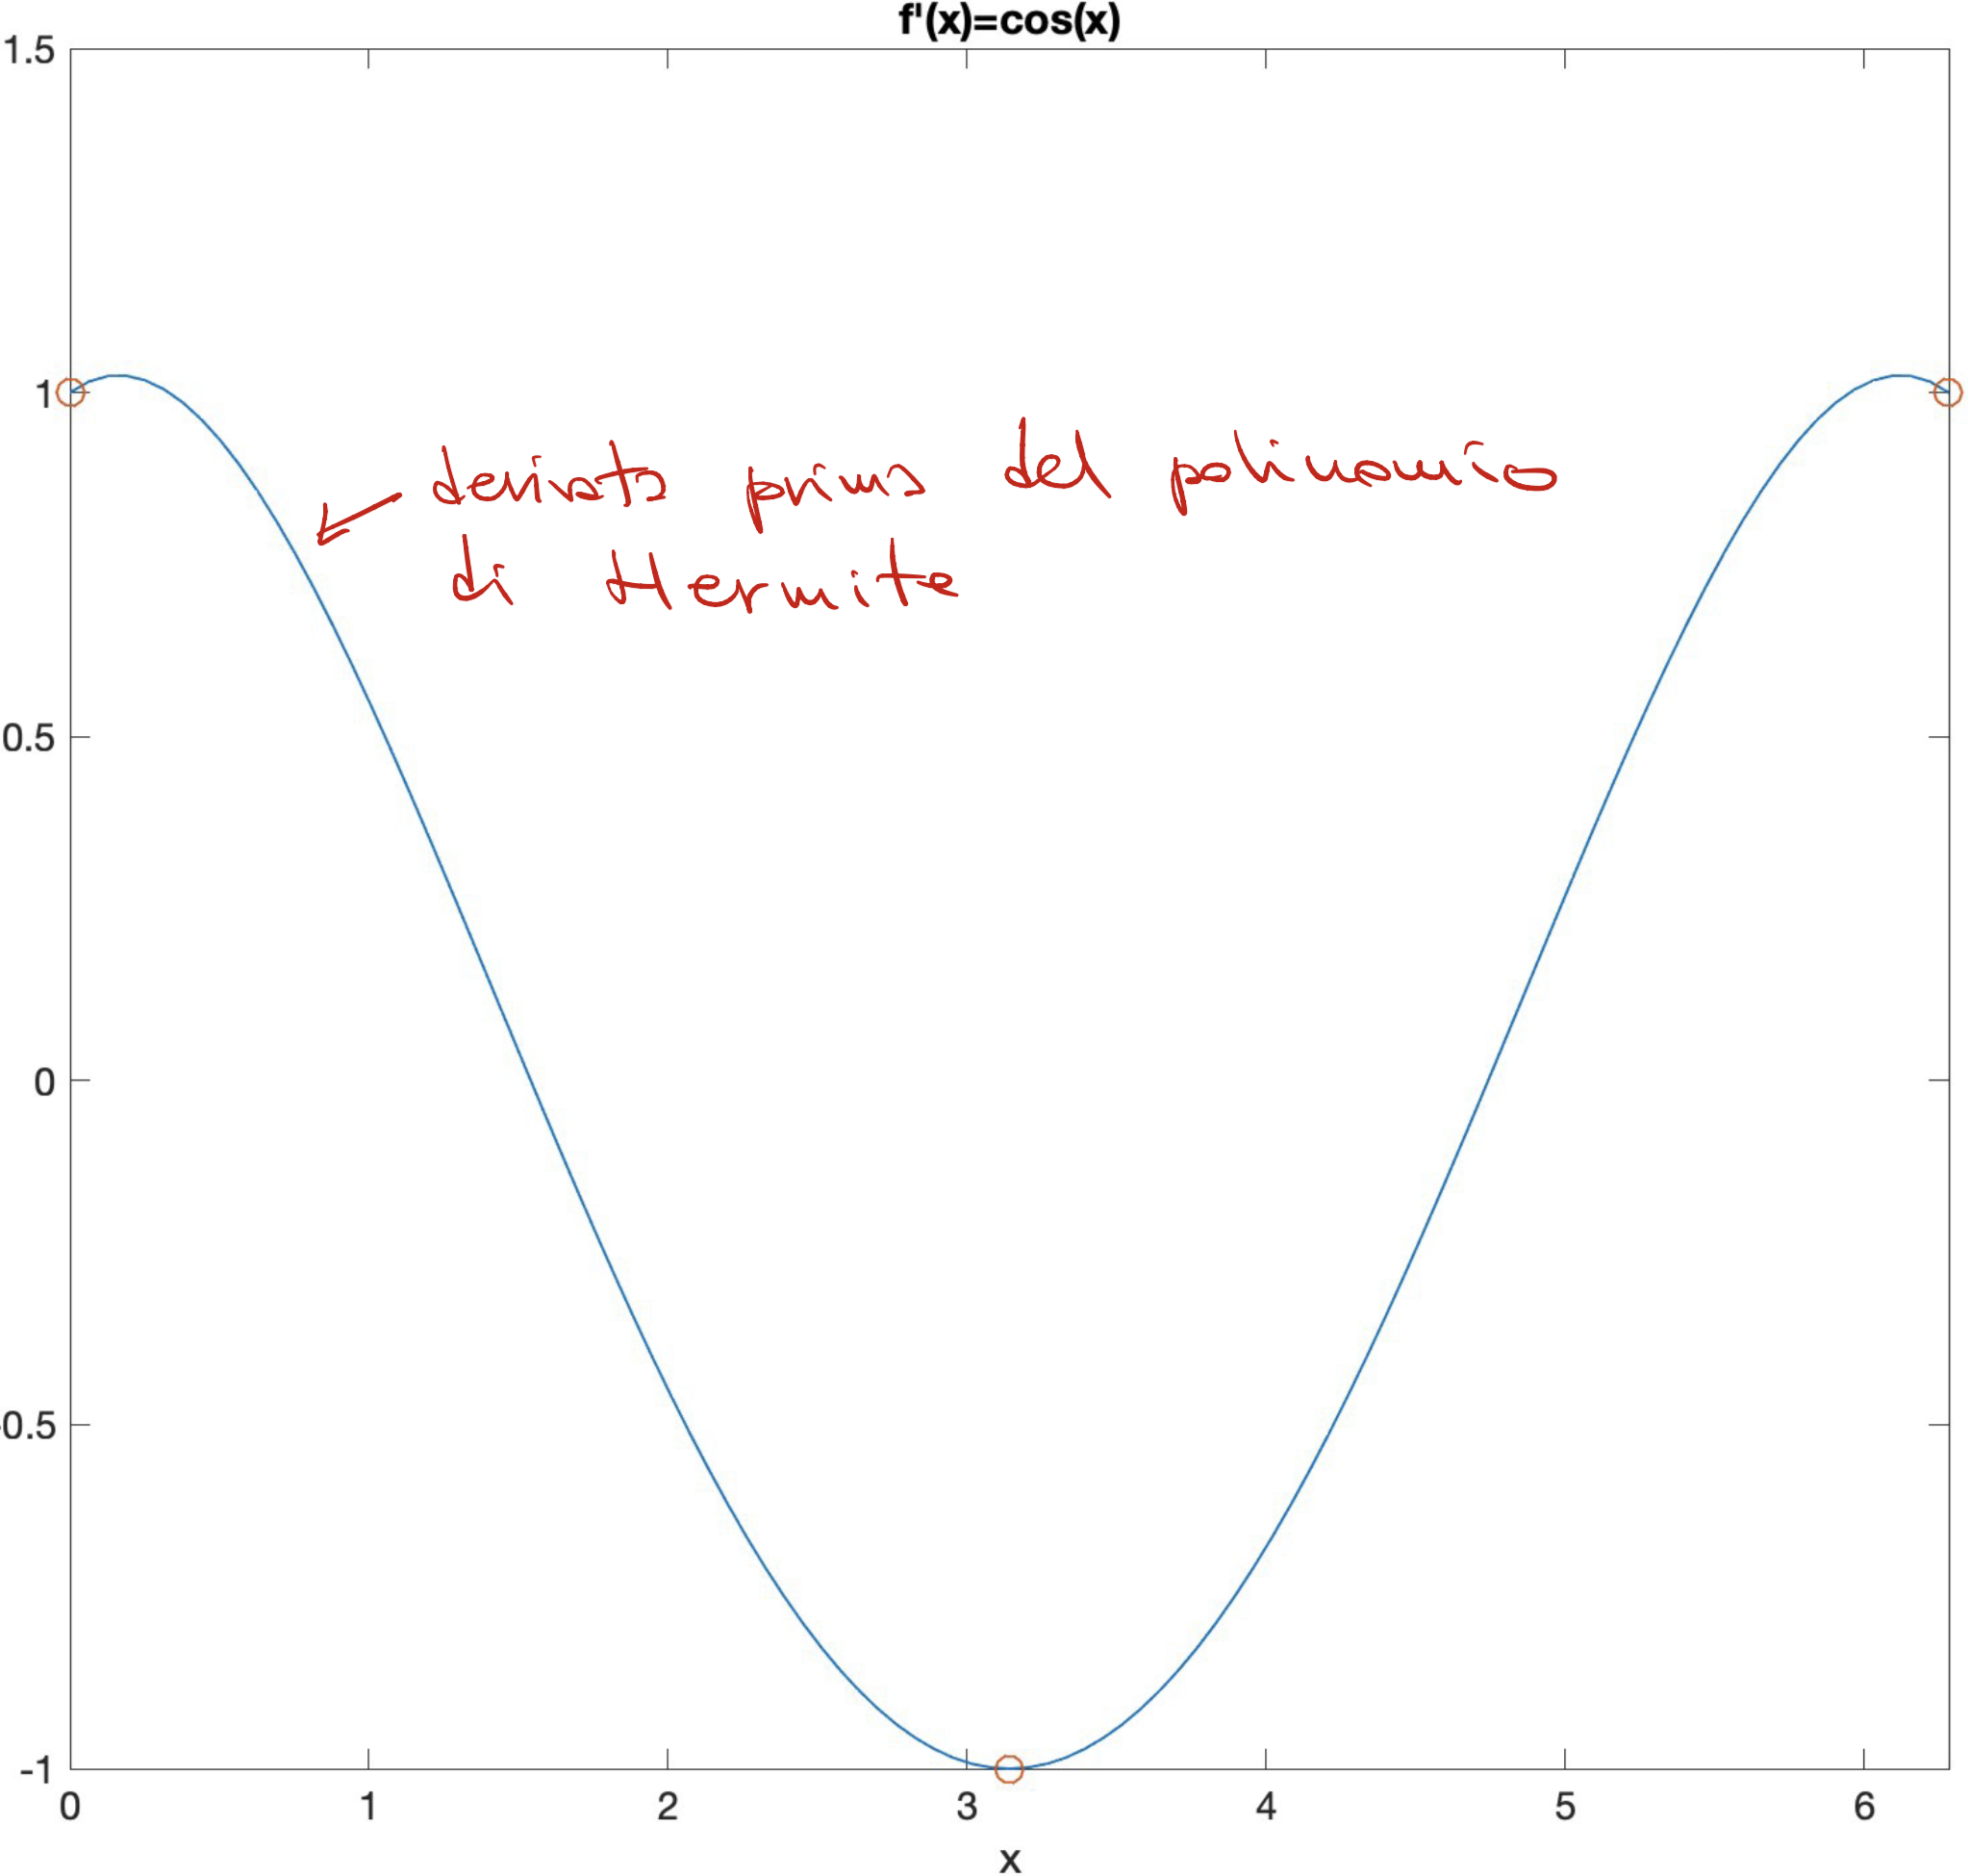
\includegraphics[width=0.5\textwidth]{immagini/PolHermite-1.png}
\caption{\label{fig:PolHermite1} Esempio delle differenze di approssimazione}
\end{figure}

\begin{remark}[Calcolo $p_H(x)$, caso semplice]
    Per il calcolo del polinomio di Hermite è utilizzata la sua forma di Newton: un caso semplice, per estrapolare una situazione generale, è con $n=2$, ovvero

    \begin{equation*}
        \begin{matrix}
            p_H(x)&=& f[x_0]\cdot 1\\
            &+& f[x_0,x_0](x-x_0)\\
            &+& f[x_0,x_0,x_1](x-x_0)^2\\
            &+& f[x_0,x_0,x_1,x_1](x-x_0)^2(x-x_1)\\
            &+& f[x_0,x_0,x_1,x_1,x_2](x-x_0)^2(x-x_1)^2\\
            &+& f[x_0,x_0,x_1,x_1,x_{\boldsymbol 2},x_{\boldsymbol 2}](x-x_0)^2(x-x_1)^2(x-x_{\boldsymbol 2}).
        \end{matrix}
    \end{equation*}
\end{remark}

Il risultato dell'osservazione è ottenuto immaginando di avere il doppio delle ascisse mediante l'utilizzo dell'indice $i+\frac{1}{2}$, dove le ascisse con questo indice tendono ad $x_i$ (analogo per le funzioni di base di Newton).
    
È importante osservare che da $f[x_0]$ è possibile arrivare a $f[x_0,x_0,x_1,x_1,x_2,x_2]$. Quest'ultima differenza divisa ha tutte le ascisse raddoppiate ed è possibile che l'ultimo polinomio di base di Newton abbia tutte le ascisse al quadrato, tranne l'$n$-esima (altrimenti avrebbe grado $2n+2$ invece di $2n+1$).

\begin{remark}[Calcolo $p_H(x)$, caso generale]
    In generale, per $\boldsymbol n$ generico, il polinomio di Hermite sarà ottenuto tramite 
    \begin{equation}\label{eq:polHerBaseNewt}
        p_H(x)=f[x_0]\cdot 1 + f[x_0,x_0]\cdot(x-x_0)+\hdots+f[x_0,x_0,\hdots,x_{\boldsymbol n},x_{\boldsymbol n}](x-x_0)^2\cdot\hdots\cdot(x-x_{\boldsymbol{n-1}})^2(x-x_{\boldsymbol n}).
    \end{equation}
    È possibile calcolare i coefficienti del polinomio, ovvero le differenze divise, con l'Algoritmo \ref{alg:calcDiffDivPolHer}, una variante dell'Algoritmo \ref{alg:calcDiffDiv}, tenendo di conto di (\ref{eq:equivApproxf'}). Nell'Algoritmo, il vettore in ingresso, \textbf{f} contiene i valori $f(x_0), f'(x_0), f(x_1), f'(x_1),\hdots, f(x_n),f'(x_n)$ ed in uscita, essendo sovrascritto, le differenze divise in (\ref{eq:polHerBaseNewt}).
\end{remark}
\begin{algorithm}
\caption{Polinomio di Hermite: calcolo delle differenze divise}\label{alg:calcDiffDivPolHer}
    \begin{lstlisting}[style=Matlab-editor]
    for i = (2*n+1):-2:3
        f(i) = (f(i)-f(i-2))/(x(i)-x(i-1))
    end
    for j = 2 : 2*n+1
        for i = (2*n+2) : -1 : j+1
            f(i) = (f(i)-f(i-1))/(x(i)-x(i-j))
        end
    end
    \end{lstlisting}
\end{algorithm}

Inoltre, è possibile calcolare $p_H(x)$ in Matlab tramite una versione modificata dell'algoritmo di Horner generalizzato (Algoritmo \ref{alg:polHornMod}), nella quale è utilizzato un vettore delle ascisse [\footnotemark] $x=[x_0\, x_0\, x_1\, x_1\, \hdots\, x_{n-1}\, x_{n-1}\,x_n]$, a patto di conoscere le differenze divise (ovvero i coefficienti del polinomio). 

\footnotetext{Le ascisse sono duplicate e per questo, nel ciclo implementato per il calcolo del polinomio, sarà contato fino ad $2n+1$. Il $+1$ è dovuto al fatto che $x_n$ è ripetuta solo una volta.}

È possibile capire come calcolare le differenze divise tramite il seguente esempio.
\begin{example}
    Considerando il caso in cui $\boldsymbol{n=1}$, il polinomio ha grado 3 seguendo la "formula" del calcolo del grado $(2n+1)$, e ritornando al caso in cui sono presenti le ascisse $x_{i+\frac{1}{2}}$ (quindi al caso in cui le ascisse sono duplicate):
    \begin{center}
        \begin{tabular}{|c|c|c|c|c|} 
        \hline
        & $\overset{\footnotemark}{0}$ & 1 & 2 & 3 \\
        \hline
        $x_0$ & $f[x_0]$ & & &\\
        $x_{\frac{1}{2}}$ & $f\left[x_\frac{1}{2}\right]$ & $f\left[\boldsymbol{x_0},\boldsymbol{x_\frac{1}{2}}\right]$ & &\\
        $x_1$ & $f[x_1]$ & $f\left[\boldsymbol{x_\frac{1}{2}},\boldsymbol{x_1}\right]$ & $f[\boldsymbol{x_0},x_{\frac{1}{2}}, \boldsymbol{x_1}]$ &\\
        $x_{\frac{3}{2}}$ & $f\left[x_\frac{3}{2}\right]$ & $f\left[\boldsymbol{x_1},\boldsymbol{x_\frac{3}{2}}\right]$ & $f\left[\boldsymbol{x_\frac{1}{2}},x_1,\boldsymbol{x_\frac{3}{2}}\right]$ & $f\left[\boldsymbol{x_0}, x_\frac{1}{2}, x_1, \boldsymbol{x_\frac{3}{2}}\right]$\\
        \hline
        \end{tabular}
    \end{center}\footnotetext{Differenza tra l'indice delle ascisse utilizzando la proprieta' incrementale delle differenze divise.}
    Le ascisse in \textbf{grassetto} sono quelle la cui differenza va a denominatore nel calcolo della rispettiva differenza divisa. 
    
    Operando il \textbf{limite} per $\boldsymbol{x_{i+\frac{1}{2}}\rightarrow x_i}$:
    \begin{center}
        \begin{tabular}{|c|c|c|c|c|} 
        \hline
        & 0 & \textbf{1} & 2 & 3 \\
        \hline
        $x_0$ & $f[x_0]$ & & &\\
        $x_0$ & $f[x_0]$ & \fbox{$f[\boldsymbol{x_0},\boldsymbol{x_0}]$} & &\\
        $x_1$ & $f[x_1]$ & $f[\boldsymbol{x_0},\boldsymbol{x_1}]$ & $f[\boldsymbol{x_0},x_0, \boldsymbol{x_1}]$ &\\
        $x_1$ & $f[x_1]$ & \fbox{$f[\boldsymbol{x_1},\boldsymbol{x_1}]$} & ${f[\boldsymbol{x_0}},x_1,\boldsymbol{x_1}]$ & $f[\boldsymbol{x_0}, x_0, x_1, \boldsymbol{x_1}]$\\
        \hline
        \end{tabular}
    \end{center}
    
    Le differenze divise cerchiate sono le differenze divise per le quali non è noto il metodo di calcolo. 
    
    Per un generico $\boldsymbol n$ non è possibile calcolare direttamente le differenze divise in colonna $\boldsymbol{1}$ \fbox{$f[x_i,x_i],\; i=0,\hdots,n,$} tuttavia è possibile quanto segue:
    \begin{equation*}
        \boldsymbol{f[x_i,x_i]}=\lim_{x_{i+\frac{1}{2}}\to x_i}\frac{f\left(x_{i+\frac{1}{2}}\right)-f(x_i)}{x_{i+\frac{1}{2}}+x_i}=\boldsymbol{f'(x_i)}.
    \end{equation*}
\end{example}

Pertanto, è possibile modificare leggermente l'algoritmo classico per il calcolo delle differenze divise (ovvero l'Algoritmo \ref{alg:calcDiffDiv}), in modo che, dove sono presenti ascisse ripetute, sia utilizzato il corrispondente valore della derivata della funzione $f(x)$, come appena esposto. In questo modo sono presenti tutti gli elementi per implementare efficientemente il calcolo del polinomio interpolante di Hermite nella sua forma di Newton.

\begin{remark}
    Nella tabella precedente, utilizzata per il calcolo delle differenze divise, il vettore delle ascisse uilizzato è del tipo $x=[x_0\, x_0\, x_1\, x_1 \hdots x_{\boldsymbol n}\, x_{\boldsymbol n}].$
\end{remark}

\subsection{Errore nell'interpolazione polinomiale}\label{ssec:errInter}\footnote{Slide 2-23 PDF 19, PG 86-87.}
È necessario studiare il comportamento della funzione errore $e$ definita come
\begin{equation}\label{eq:defErrInter}
    \boldsymbol{e(x)=f(x)-p(x)},\quad x\in [a,b],
\end{equation}
per la quale è possibile osservare che $f(x)=p(x)+e(x)$, con $e(x)$ errore commesso nell'approssimazione di $f(x)$ tramite il polinomio interpolante $p(x)$.

\begin{figure}
    \centering
    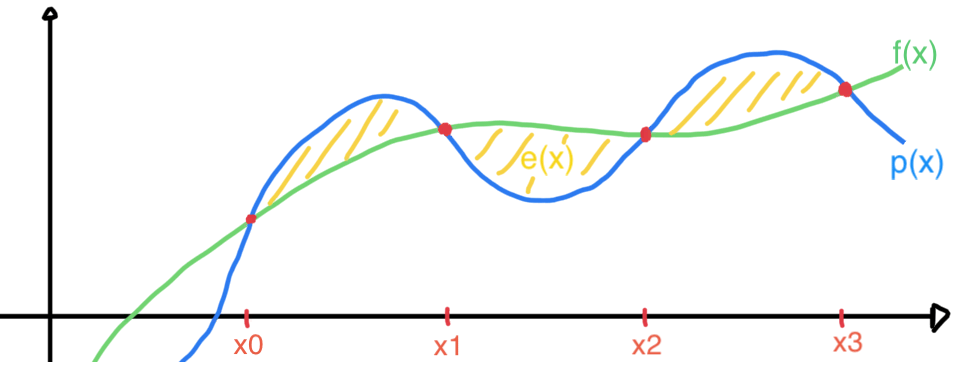
\includegraphics[width=0.5\textwidth]{immagini/ErrorePolinomioHermite.png}
    \caption{Esempio dell'errore $e$ del polinomio Hermite $p$ rispetto a $f$.}
    \label{fig:errPolHer}
\end{figure}
 
\begin{remark}
    \footnote{Slide 3, PDF 19. Da (\ref{eq:condInterp}) segue l'osservazione.} $e(x_i)=f(x_i)-p(x_i)=f(x_i)-f(x_i)=0,\; i=0,\hdots,n.$
\end{remark}

Pertanto, è noto che nelle ascisse di interpolazione l'errore si annulla. È necessario stabilire quanto $e(x)$ sia "distante" da 0, per $x\notin \{x_0,\hdots, x_n\}.$

\begin{theorem}\label{th:errInterFormaNewt}
    \footnote{Slide 3 PDF 19, TH 4.3 PG 86.} Dato $p(x)$, polinomio interpolante $f(x)$, definito come (\ref{eq:polInterNewt}), sulle ascisse distinte (definite come in (\ref{eq:ascisseDistinte})), vale:
    \begin{equation}\label{eq:errInterFormaNewt}
        \boldsymbol{e(x)=f[x_0,x_1,\hdots,x_n,x]\,\omega_{n+1}(x),\quad w_{n+1}(x)=\prod_{j=0}^{n}(x-x_j)}.
    \end{equation}
\end{theorem}

\begin{proof}
    \footnote{Sfrutta il fatto che è possibile costruire il polinomio interpolante nella forma di Newton in modo incrementale.} Fissato $\widehat x\notin\overbrace{\{x_0,\hdots,x_n\}}^{\text{ascisse d'interp.}}$ un punto generico, il polinomio $\widehat p(x)\in\Pi_{n+1}$ è costruito come segue:
    \begin{equation*}
        \begin{matrix}
            \widehat p(x_i)&=&f(x_i),& i=0,\hdots,n,\\
        \widehat p(\widehat x) &=& f(\widehat x),
        \end{matrix}
    \end{equation*}
    Ovvero, $\widehat p(x)$ interpola $f(x)$ anche in $\widehat x$, oltre che nelle ascisse $x_0,\hdots,x_n$.
    
    (È imposta la seguente condizione:) Utilizzando la forma di Newton del polinomio interpolante (Teorema \ref{th:formaNewt}) è ottenuto che
    \begin{equation*}
        \underset{\footnotemark}{\widehat p(x)} = p(x) + f[x_0,\hdots,x_n,\widehat x]\,\omega_{n+1}(x),
    \end{equation*}
    la quale soddisfa le condizioni di interpolazione
    \begin{equation*}
        \widehat p(x_i)=\equalto{p(x_i)}{f(x_i)} + f[x_0,\hdots,x_n,\widehat x]\,\overbrace{\omega_{n+1}(x_i)}^{0} \boldsymbol = f(x_i),\quad i=0,\hdots,n,
    \end{equation*}
    ed inoltre:
    \begin{equation*}
        \widehat p(\widehat x)=p(\widehat x)+ f[x_0,\hdots,x_n,\widehat x]\,\omega_{n+1}(\widehat x)\boldsymbol = f(\widehat x).
    \end{equation*}
    Da quest'ultima uguaglianza è ottenuto che
    \begin{equation*}
        \boldsymbol{e(\widehat x)\equiv} \underbrace{f(\widehat x) - p(\widehat x)}_{\text{errore di $\widehat x$}}=f[x_0,\hdots,x_n,\widehat x]\,\omega_{n+1}(\widehat x).
    \end{equation*}
    L'aaserto discende dal fatto che $\widehat x$ è un punto generico. [\footnotemark]
\end{proof}

\addtocounter{footnote}{-1}
\footnotetext{Quando è calcolato in una delle ascisse $x_i$, si annulla sia il polinomio di interpolazione che la funzione. Il coefficiente $f[x_0,\hdots,x_n,\widehat x]$ permette di ottenere le seguenti condizioni di accuratezza (ovvero le condizioni di interpolazione che seguono).}

\stepcounter{footnote}
\footnotetext{Se al posto di $\widehat x$ è sostituito $x$ allora $\widehat p(x)$ continua a variare.}

\begin{remark}
    Il Teorema \ref{th:errInterFormaNewt} definisce la forma dell'errore di interpolazione polinomiale (e di conseguenza è necessario impararlo).
\end{remark}

\begin{corollary}
    \footnote{Slide 5 PDF 19, Corollario 4.1 PG 87; Importante perché esiste un legame tra le differenze divise e le derivate della funzione $f$, se questa è sufficientemente regolare.}
    Utilizzando le ipotesi del Teorema \ref{th:errInterFormaNewt} e supposto che $f\in C^{(n+1)}$ sul più piccolo intervallo contenente le ascisse in argomento alla differenza divisa in (\ref{eq:errInterFormaNewt}), allora (vedere (\ref{eq:P4DiffDiv})):
    \begin{equation}\label{eq:errInterP4}
        \begin{matrix}
            e(x)=\frac{f^{(n+1)}(\xi_x)}{(n+1)!}\,\omega_{n+1}(x),&\\
            &\xi_x\in[\min\{\underset{i}{\min}\,x_i,\,x\},\, \max\{\underset{i}{\max}\,x_i,\, x\}]\boldsymbol{\equiv I(x)}.
        \end{matrix}
    \end{equation}
\end{corollary}

\begin{remark}[Errore polinomio di Hermite]\label{rem:errPolHerm}
    \footnote{Da sapere. Slide 5 PDF 19, Oss. 4.4 PG 87.}
    Per il polinomio di Hermite (\ref{eq:polHerBaseNewt}) interpolante la funzione $f(x)\left(\in C^{(2n+2)}[I(x)]\right)$, sulle ascisse $x_0,\hdots,x_n$, l'errore corrispondente al polinomio è definito come
    \begin{equation}\label{eq:errPolInterHer}
        e_H(x)= f(x)-p_H(x) \overset{\footnotemark}{=} f[\overbrace{x_0,x_0,\hdots,x_n,x_n,x}^{2n+3}]\,\omega^2_{n+1}(x)\equiv\frac{\boxed{f^{(2n+2)}(\widehat\xi_x)}}{(2n+2)!}\,\omega^2_{n+1}(x).
    \end{equation}
\end{remark}
$e_H(x)$ è di grado $2n+2$.
\footnotetext{Le funzioni di base del polinomio di Newton hanno ascisse raddoppiate.}

\begin{remark}\footnote{Slide 5 PDF 19.}
    Da quanto esposto nell'Osservazione \ref{rem:errPolHerm} è ottenuta una controprova del fatto che:
    \begin{enumerate}
        \item $p(x)\equiv f(x),\; \text{se } f(x)\in\Pi_n\; \left(f^{(n+1)}\equiv 0\right)$;
        \item $p_H(x)\equiv f(x),\; \text{se } f(x)\in\Pi_{2n+1}\; \left(f^{(2n+2)}\equiv 0\right)$.
    \end{enumerate}
\end{remark}

\begin{remark}\label{rem:consErrInterP4}\footnote{Slide 6 PDF 19.}
    Osservando la struttura dell'errore (\ref{eq:errInterP4})
    \begin{center}
        $e(x)=\,\boxed{\boxed{\frac{f^{(n+1)}(\xi_x)}{(n+1)!}}\;\boxed{\omega_{n+1}(x)}}$
    \end{center}
\end{remark}
(analoghe considerazioni varranno per $e_H(x)$), è possibile osservare che questo è costituito da due parti:
\begin{itemize}
    \item la prima che dipende da $\boxed{f(x)}$, per cui, più $f(x)$ è regolare, tanto più velocemente questo termine tende a 0, per $n\rightarrow\infty$ (dovuto a $(n+1)!$ al denominatore);
    \item la seconda, $\boxed{\omega_{n+1}(x)=\prod_{j=0}^n(x-x_j)}$, dipende solo dalla scelta delle ascisse di interpolazione.
    
    È necessario osservare che, per $x>\underset{i}{\max}\{x_i\}$ o per $x<\underset{i}{\min}\{x_i\},\, \omega_{n+1}(x)\approx x^{n+1}$ (vedere Figura \ref{fig:ossErrInterp}). Da questa considerazione è evinto che $x$ debba essere scelta nel più piccolo intervallo che contiene le ascisse di interpolazione (in Figura \ref{fig:ossErrInterp} tra $x_0$ e $x_2$). \textbf{Quindi sarà scelta $\boldsymbol{x\in [a,b]}$ che contiene le ascisse}.
\end{itemize}

\begin{figure}
    \centering
    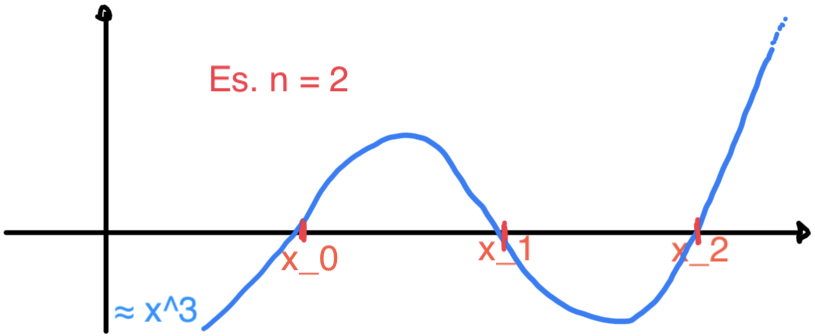
\includegraphics[width=0.5\textwidth]{immagini/es. n=2.png}
    \caption{\label{fig:ossErrInterp} Esempio con numero di ascisse $n=2$.}
\end{figure}

Il polinomio interpolante coincide con la funzione $f$, come per il riquadro principale di $e(x)$ nell'Osservazione \ref{rem:consErrInterP4}, se $f$ è un polinomio di grado al più $n$ con la sua derivata $(n+1)$-esima che si annulla identicamente. Quindi, se la funzione $f$ è un polinomio di grado al più $n$ l'errore è identicamente nullo, il che significa che il polinomio interpolante coincide con la funzione di Hermite (ovvero l'uguaglianza (\ref{eq:errPolInterHer})).

Data l'interpolazione di Hermite su $n+1$ ascisse (il polinomio interpolante di Hermite è di grado $2n+1$), se la funzione interpolante è un polinomio di grado al più $2n+1$, ancora una volta, il polinomio di Hermite coinciderà con la funzione interpolante. Ciò viene confermato dalla parte riquadrata in (\ref{eq:errPolInterHer}), in quanto la derivata $(2n+1)$-esima di un polinomio di grado $2n+1$ è identicamente nulla.

Con funzioni "buone" è possibile aspettarsi che $p(x)$ approssimi sempre meglio $f(x)$, per $n\rightarrow\infty$.

Come misura dell'errore, negli esempi che seguono, è considerata la norma infinito:
\begin{equation*}
    ||e||\overset{\footnotemark}{=} \overbrace{\underset{\boldsymbol{a\leq x\leq b}}{\max}|\underbrace{f(x)-p(x)}_{e(x)}|}^{\footnotemark}\approx \underset{\boldsymbol{x=a+i\frac{b-a}{N},\, i=0,\hdots,N}}{\max}|e(x_i)|,\quad N>>1\; (N=\boldsymbol{10000}).
\end{equation*}
\addtocounter{footnote}{-1}
\footnotetext{Norma uniforme, ovvero continua nell'intervallo $[a,b]$.}
\stepcounter{footnote}
\footnotetext{Che è una norma in $C^{(0)}[a,b]$.}

$||e||$ sarà approssimata, dato che non è possibile calcolarla, con la differenza in valore assoluto, calcolato su un numero molto ampio di ascisse. $||e||$ è una sottostima ed è buona se è utilizzato un numero accettabile di punti ($N>10000$).

\paragraph{Progetto e scelta di $N$:} Per il progetto $N$ deve essere molto grande. Negli esempi richiesti nell'elaborato non saranno ammessi $N<10000$ (saranno considerati sbagliati). Inoltre, per un polinomio di grado 5 assegnare $N=3$ sarà considerato sbagliato in quanto la sottostima dell'errore è importante.

\begin{example}
    Per $f(x)=\sin(x)$ è possibile ottenere ottimi risultati (vedere Figure \ref{fig:approxErrIntepolaz4}-\ref{fig:approxErrIntepolaz19}), utilizzando un numero di ascisse crescenti ed equidistanti, dato che tutte le derivate di $\sin(x)$ sono limitate.

    Date le Figure \ref{fig:approxErrIntepolaz4}-\ref{fig:approxErrIntepolaz19}, per $f(x)=\sin(x)$, è ottenuto un numero crescente di ascisse equidistanti, dato che le derivate di $\sin(x)$ sono tutte limitate.
\end{example}

\begin{figure}%[H]
\centering
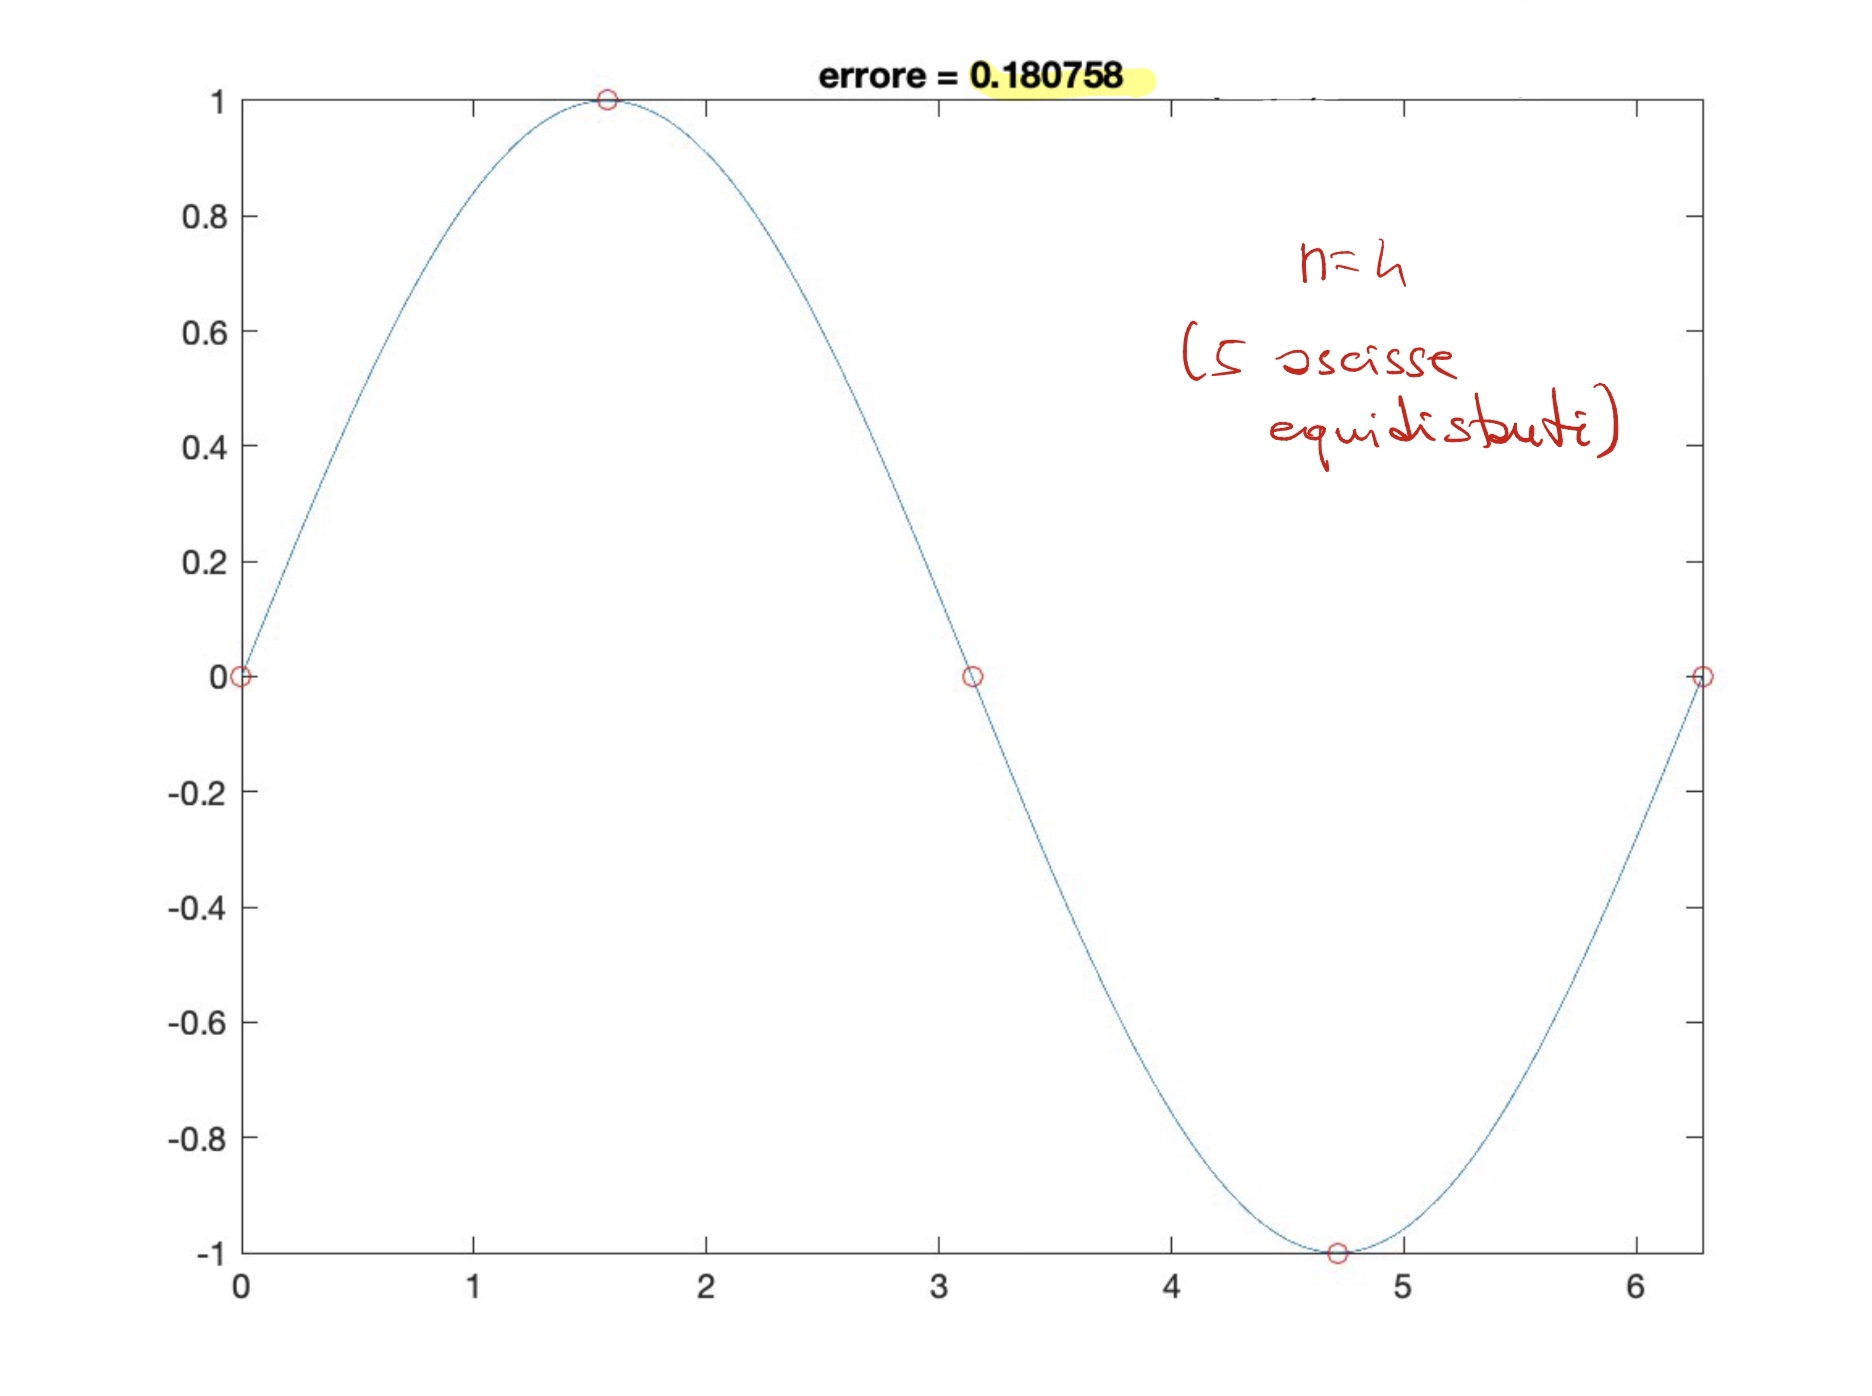
\includegraphics[width=0.55\textwidth]{immagini/sin(n=4).jpg}
\caption{Esempio con numero di ascisse $n=4$.}\label{fig:approxErrIntepolaz4}
\end{figure}

\begin{figure}%[H]
\centering
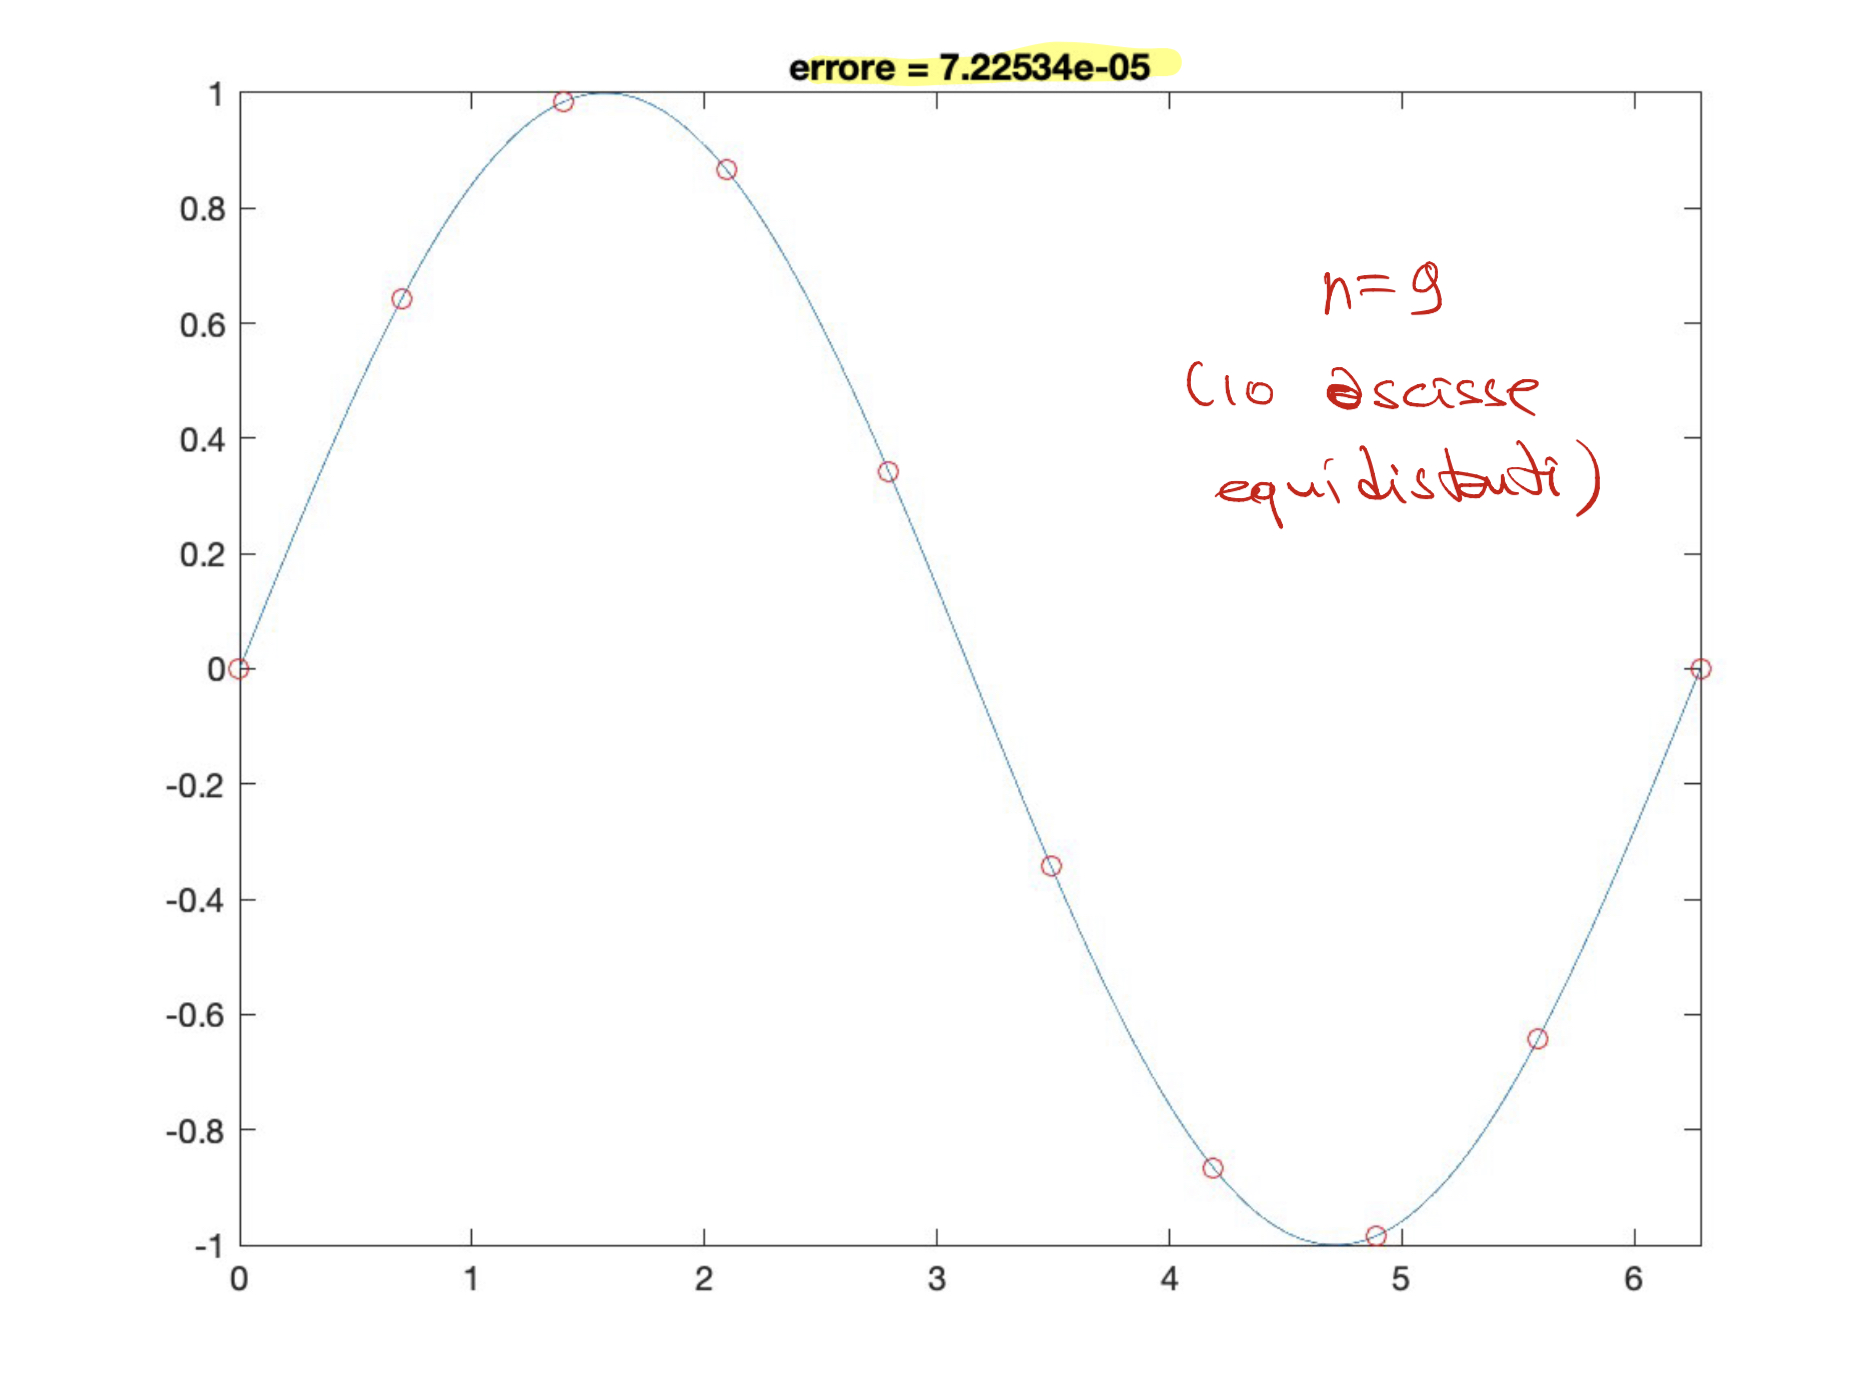
\includegraphics[width=0.5\textwidth]{immagini/sin(n=9).jpg}
\caption{Esempio con numero di ascisse $n=9$.}\label{fig:approxErrIntepolaz9}
\end{figure}

\begin{figure}%[H]
\centering
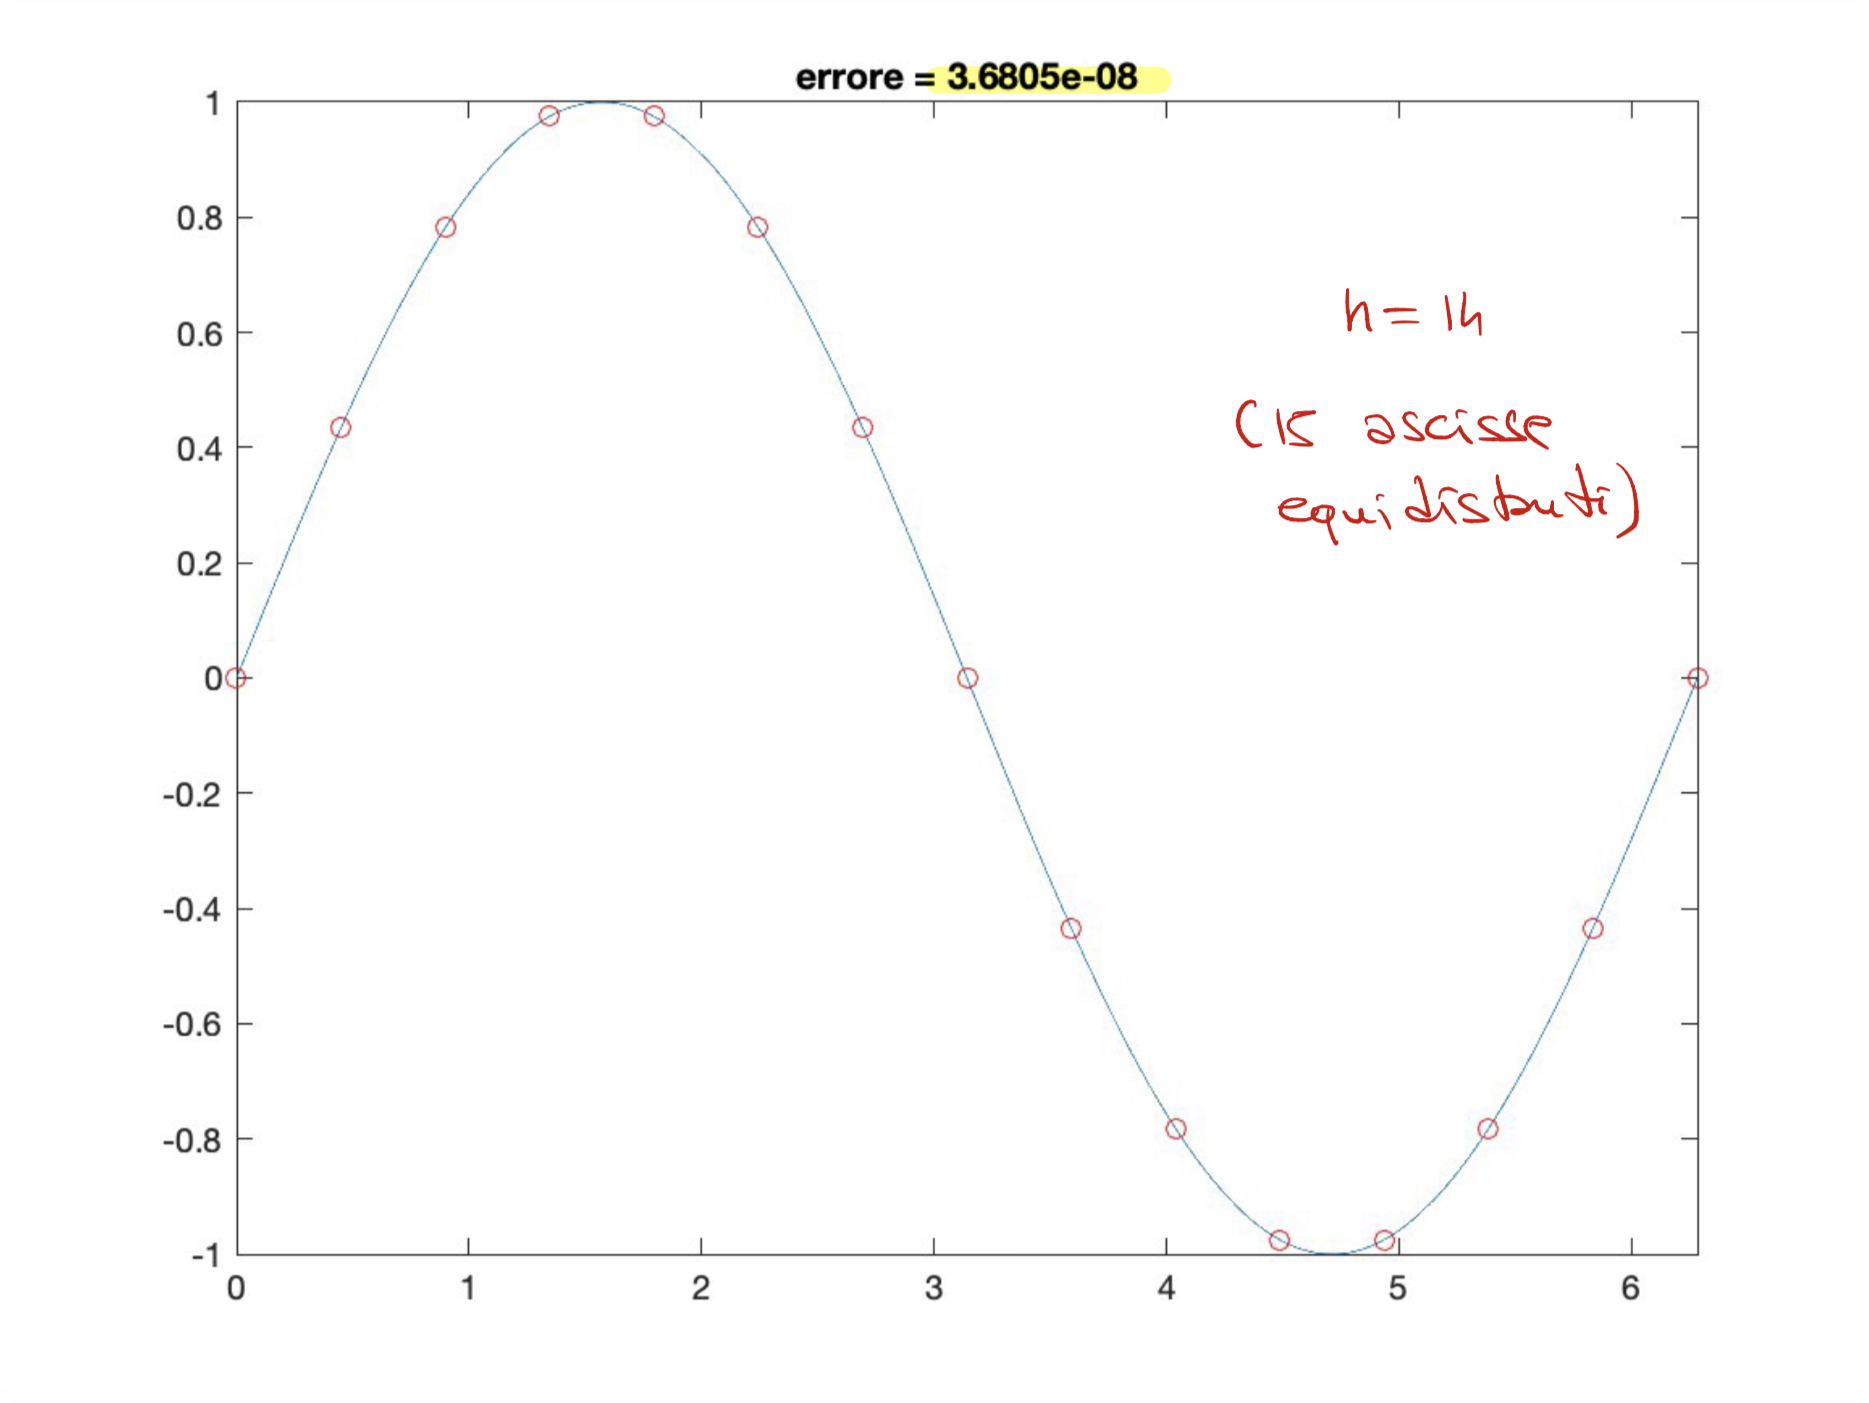
\includegraphics[width=0.5\textwidth]{immagini/sin(n=14).jpg}
\caption{Esempio con numero di ascisse $n=14$.}\label{fig:approxErrIntepolaz14}
\end{figure}

\begin{figure}%[H]
\centering
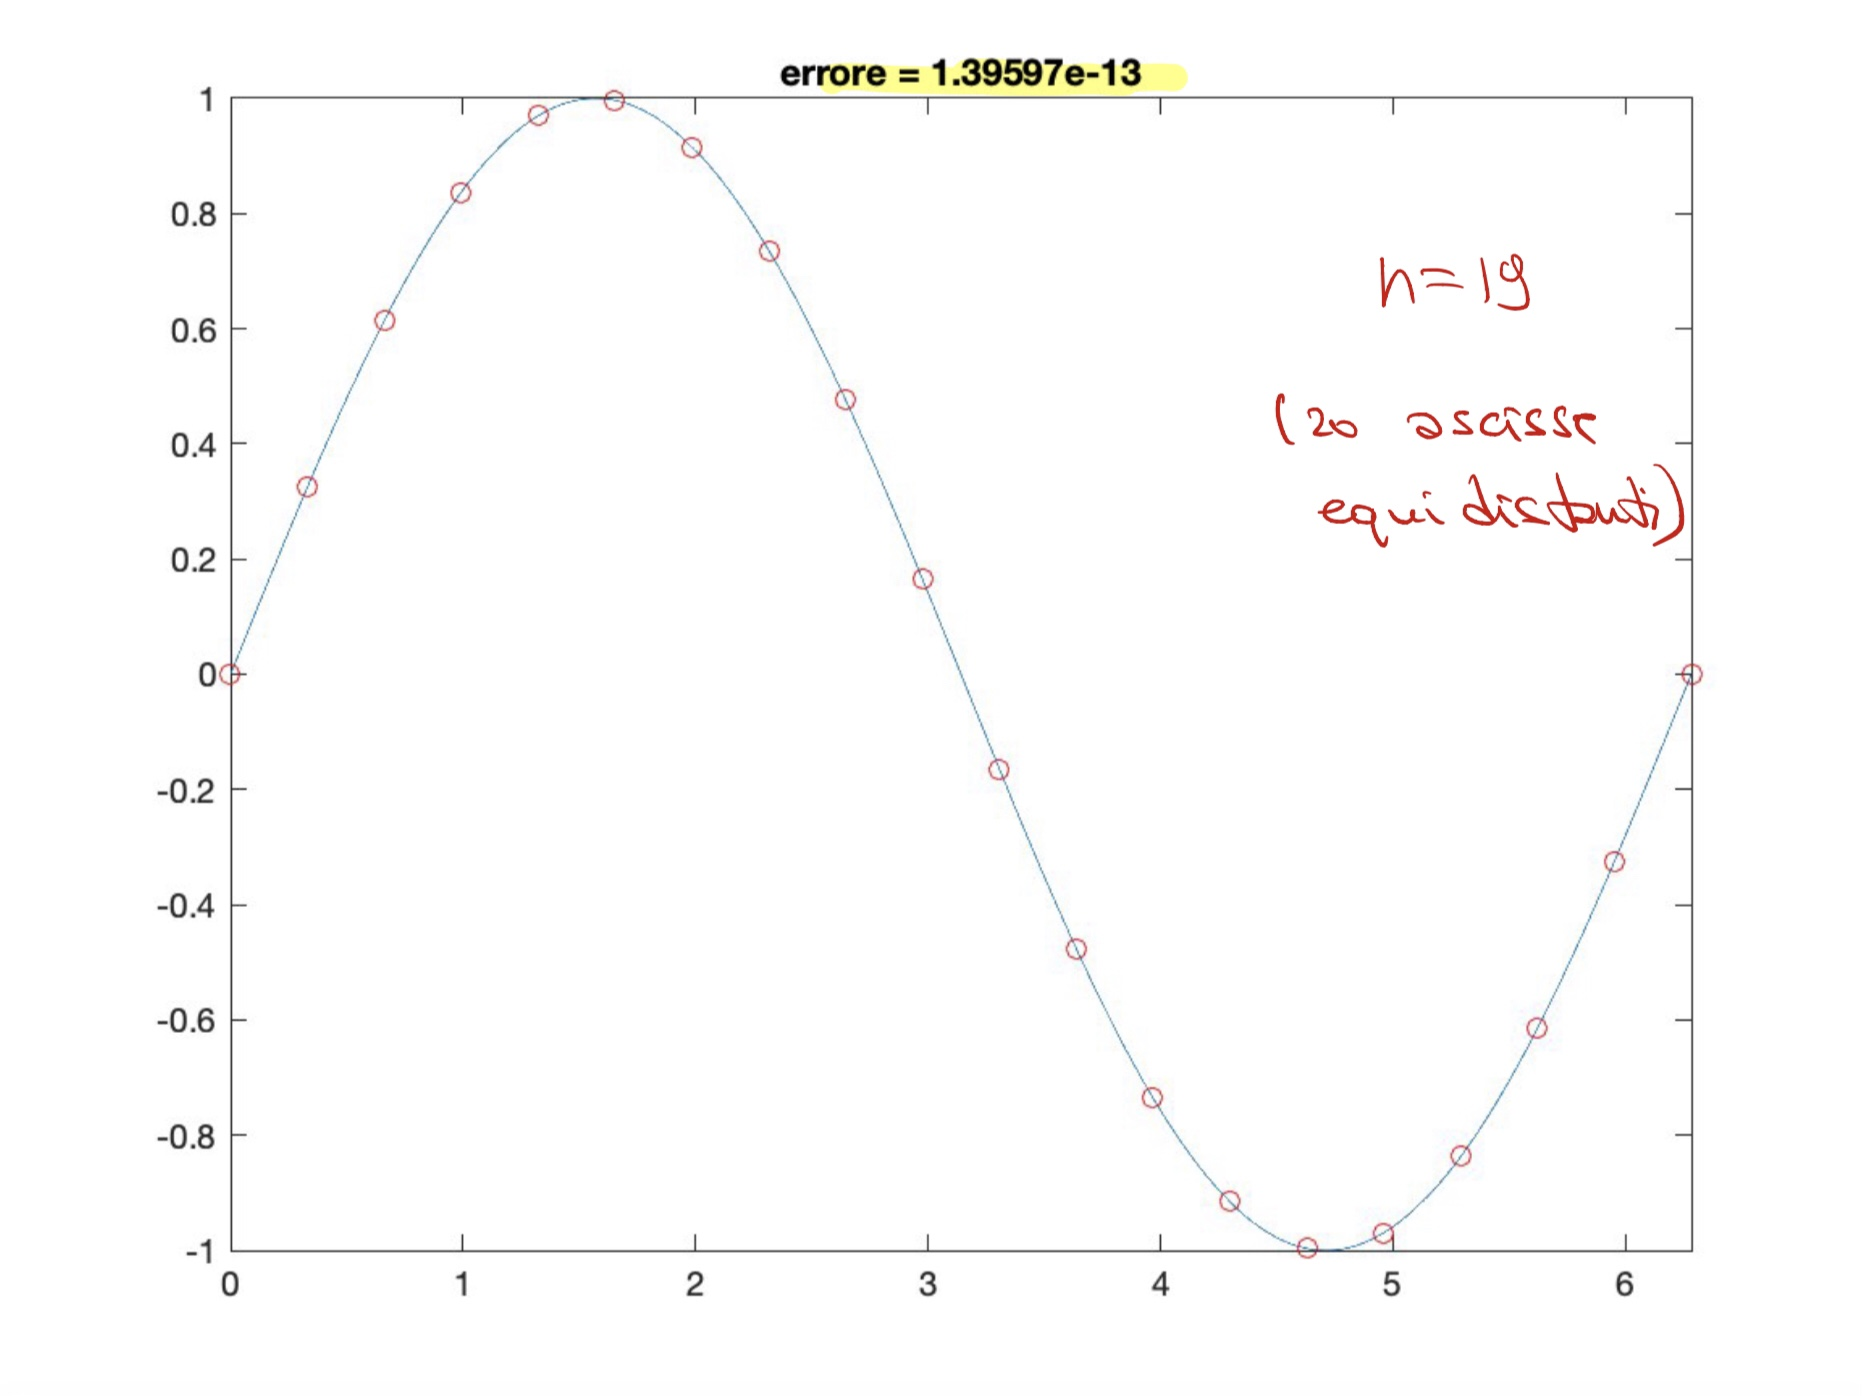
\includegraphics[width=0.5\textwidth]{immagini/sin(n=19).jpg}
\caption{Esempio con numero di ascisse $n=19$.}\label{fig:approxErrIntepolaz19}
\end{figure}

È possibile provare, come nel precedente esempio, appplicare un numero di ascisse crescenti ed equidistanti, applicando la formula di Runge, alla seguente funzione (grafico  Figura \ref{fig:funzRunge-5,5}):
\begin{equation}\label{eq:funzExRunge}
    f(x)\overset{\footnotemark}{=}\frac{1}{1+x^2},\quad x\in [-5,5].
\end{equation}

\footnotetext{Simmetrica rispetto all'asse $y$ e massimo in $x=0$, vedere Figura \ref{fig:funzRunge-5,5}.}

\begin{figure}
    \centering
    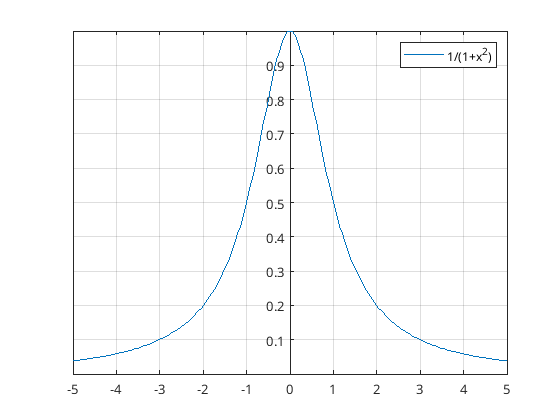
\includegraphics[width=0.5\textwidth]{immagini/funzioneRunge-5,5.png}
    \caption{Grafico di (\ref{eq:funzExRunge})}\label{fig:funzRunge-5,5}
\end{figure}

Nelle Figure \ref{fig:funzRunge_n=2}-\ref{fig:funzRunge_n=22} [\footnote{Nelle figure i puntini rappresentano la funzione di Runge.}] è utilizzata la funzione di Runge per approssimare (\ref{eq:funzExRunge}), con un numero crescente di ascisse equidistanti.

\begin{figure}
    \centering
    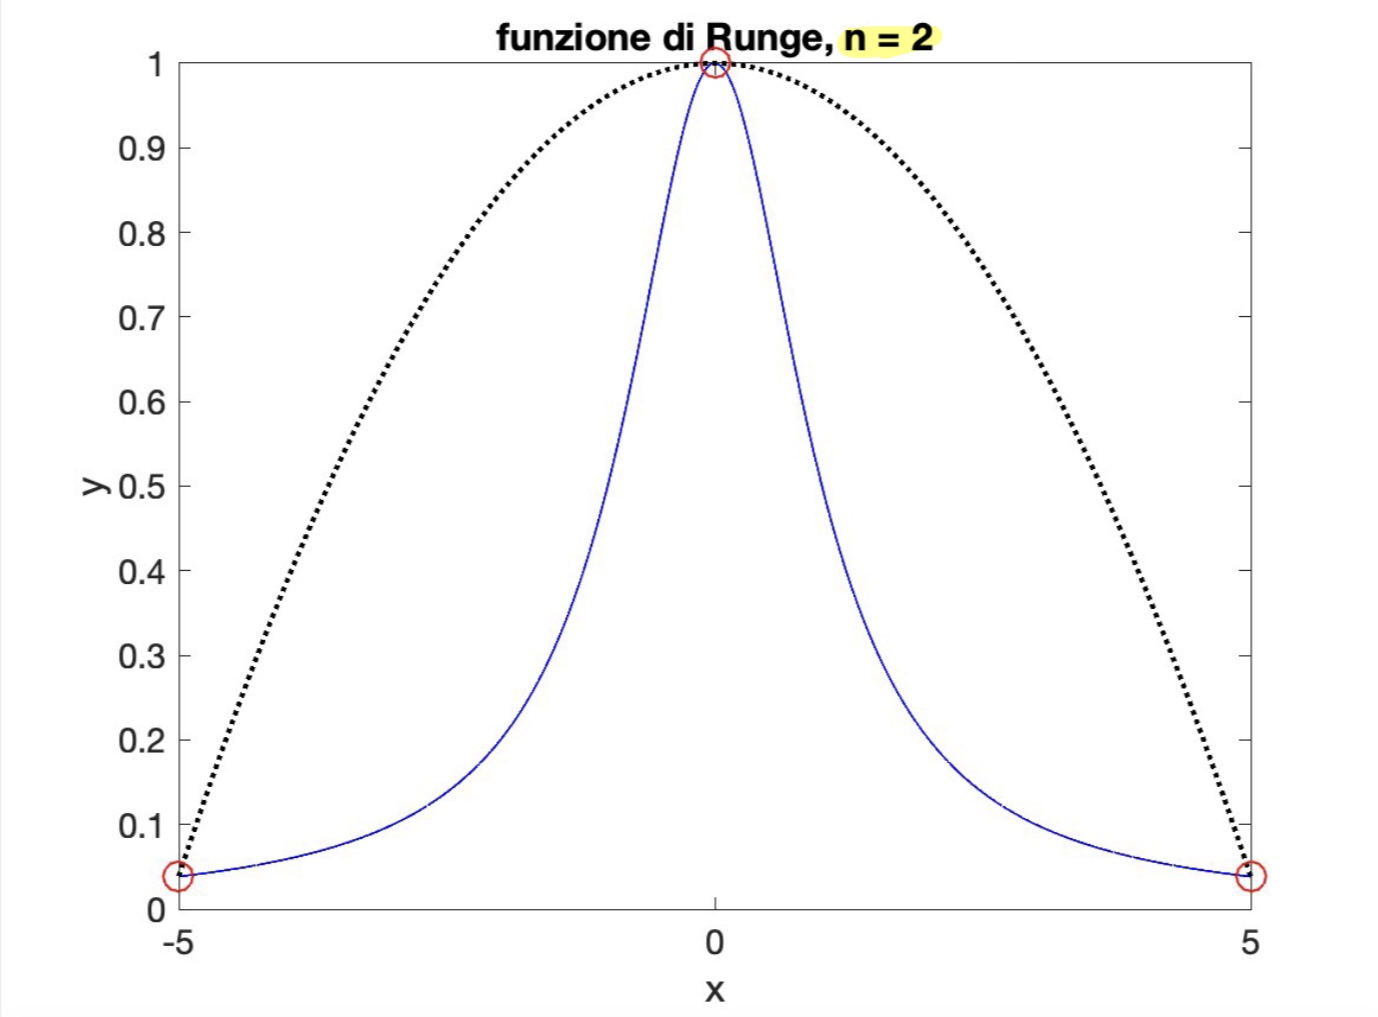
\includegraphics[width=0.5\textwidth]{immagini/funzioneRunge_n=2.jpg}
    \caption{Approssimazione di (\ref{eq:funzExRunge})}\label{fig:funzRunge_n=2}
\end{figure}
\begin{figure}
    \centering
    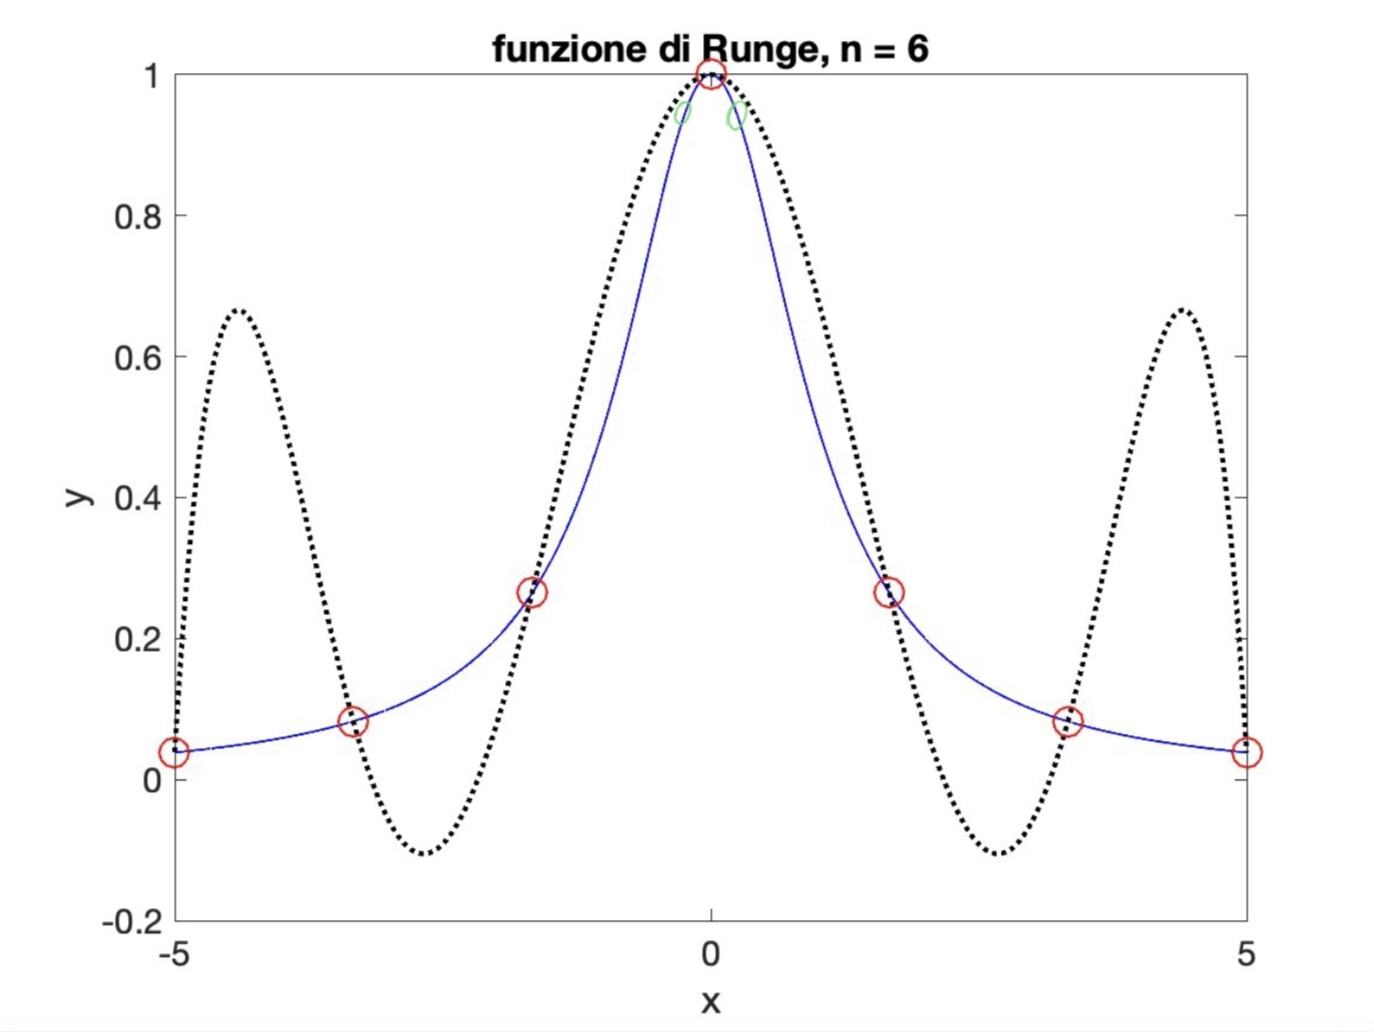
\includegraphics[width=0.5\textwidth]{immagini/funzioneRunge_n=6.jpg}
    \caption{Approssimazione di (\ref{eq:funzExRunge})}\label{fig:funzRunge_n=6}
\end{figure}
\begin{figure}
    \centering
    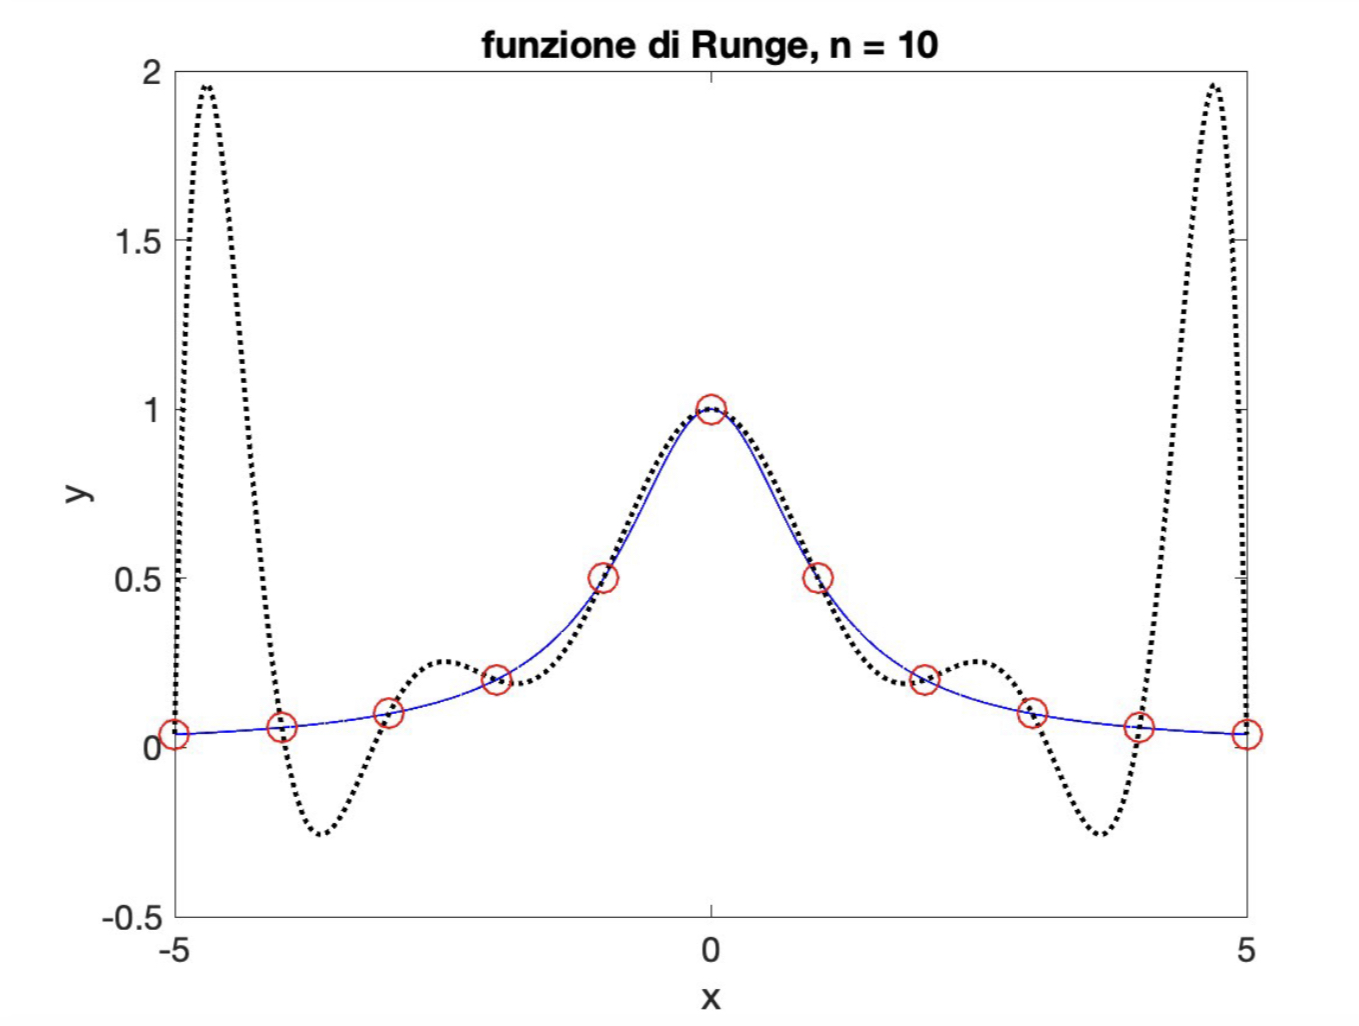
\includegraphics[width=0.5\textwidth]{immagini/funzioneRunge_n=10.jpg}
    \caption{Approssimazione di (\ref{eq:funzExRunge})}\label{fig:funzRunge_n=10}
\end{figure}
\begin{figure}
    \centering
    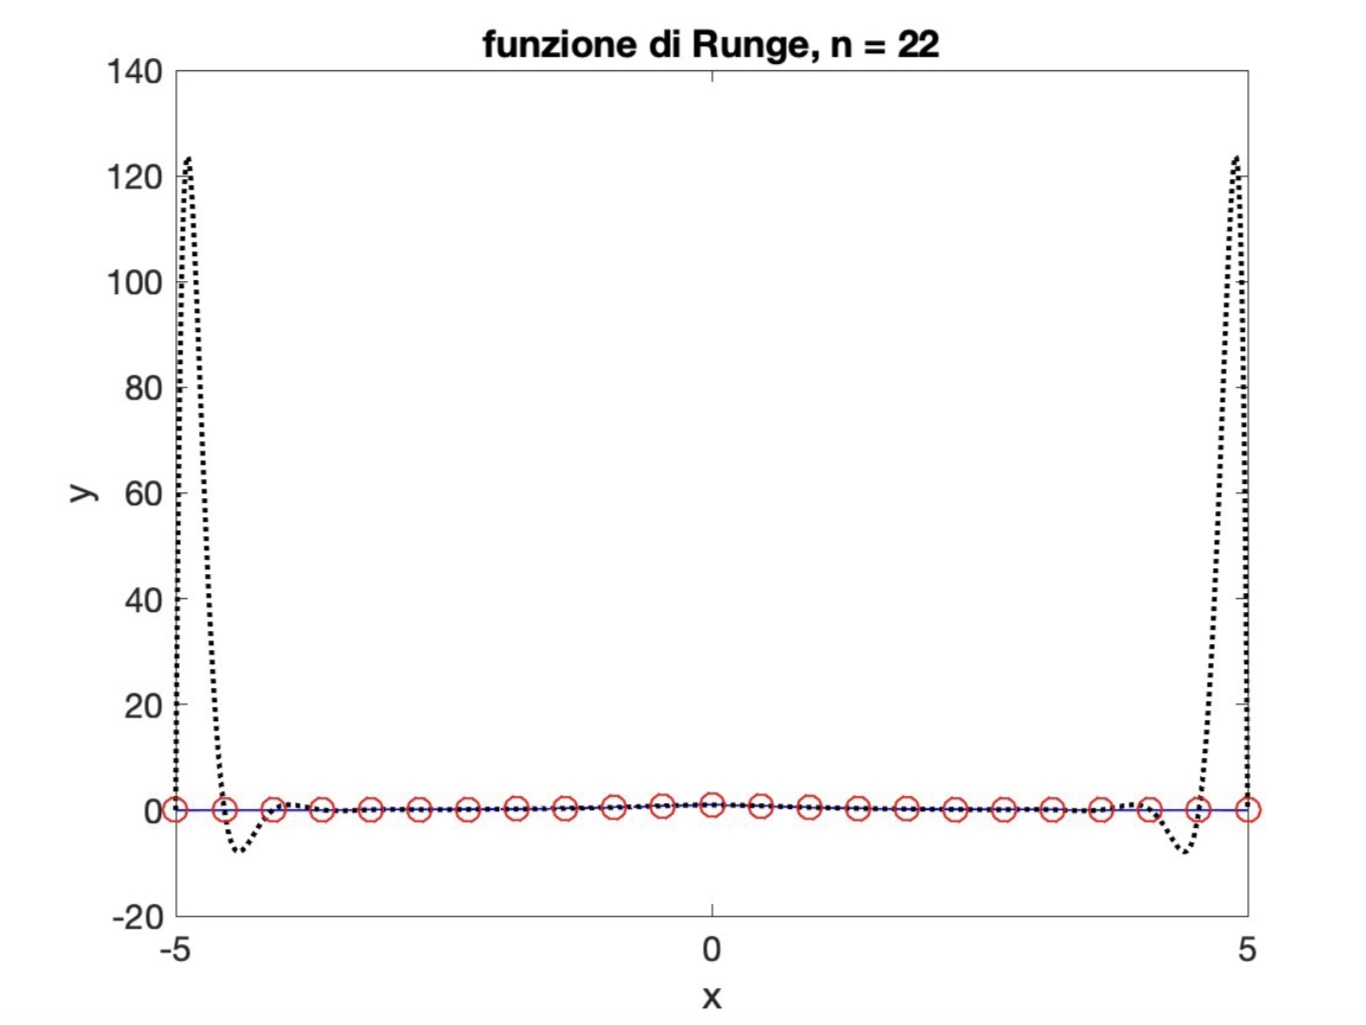
\includegraphics[width=0.5\textwidth]{immagini/funzioneRunge_n=22.jpg}
    \caption{Approssimazione di (\ref{eq:funzExRunge})}\label{fig:funzRunge_n=22}
\end{figure}

\begin{remark}[Dettagli impotanti per il progetto]
    Distinguere fra numeri pari e dispari di ascisse è importante. Se $n$ è pari allora  le ascisse sono dispari. Un esempio è graficare il polinomio (\ref{eq:funzExRunge}) per un valore pari di $n$, quindi con un numero dispari di ascisse (ovvero $n+1$), così da trovare i punti cerchiati in rosso delle Figure \ref{fig:funzRunge_n=2}-\ref{fig:funzRunge_n=22} con un metodo affidabile.  Avere un numero di ascisse dispari permette di trovare il massimo della funzione in modo più efficace rispetto ad avere un numero pari di ascisse (vedere Figura \ref{fig:funzRunge_n=6}). Inoltre, nel caso del numero di ascisse pari, l'errore diventa importante (una parte di funzione viene tagliata fuori).
\end{remark}

In genere è possibile verificare che $e(x)\rightarrow\infty,\;\, n\rightarrow\infty$, quindi il problema è malcodizionato. Tuttavia, è necessario studiare il condizionamento del problema dell'interpolazione dove, per ciascuna delle classi di problemi considerati, è noto quale sia il coefficiente di perturbazione del problema.

È necessario studiare il problema del condizionamento dell'interpolazione polinomiale, ovvero: date le ascisse di interpolazione (\ref{eq:ascisseDistinte}), è definito il polinomio $p(x)\in\Pi_n$ interpolante la funzione $f(x)\in\Pi_n$ come
\begin{equation*}
 \boldsymbol{p(x_i)=f(x_i)},\quad\boldsymbol{i=0,\hdots,n}.
\end{equation*}

Considerando una funzione $\Tilde{f}(x)$, perturbazione di $f(x)$, e costruito $\tilde{p}(x)$, il polinomio interpolante $\Tilde{f}(x)$ sulle ascisse (\ref{eq:ascisseDistinte}), come
\begin{equation*}
 \boldsymbol{\tilde{p}(x_i)=\tilde{f}(x_i),\quad i=0,\hdots,n},
\end{equation*}
allora sono introdotte le seguenti misure degli errori:

\begin{itemize}
    \item $||f-\Tilde{f}||$, misura degli errori sui dati di ingresso;
    \item $||p-\Tilde{p}||$, misura degli errori sul risultato (minore è migliore è il condizionamento del problema).
\end{itemize}

Il problema riguarda anche come sono scelte le ascisse di interpolazione.

\subsection{Condizionamento del problema}\label{ssec:condProbApproxfun}
Il problema del condizionamento dell'errore prima citato può essere "trasformato" nello studio di come $||p-\Tilde{p}||$ dipenda da $||f-\Tilde{f}||$. Studiare il condizionamento del problema significa stabilire in che modo piccole perturbazioni del problema, ovvero $||f-\Tilde{f}||$, si riflettano con perturbazioni sul risultato, ovvero su $||p-\Tilde{p}||$:
\begin{itemize}
    \item se le perturbazioni sul risultato sono piccole allora il problema è ben condizionato;
    \item se piccole perturbazioni ne provacano di grandi sul risultato il problema è malcondizionato.
\end{itemize}

Ciò che sarà studiato è il problema della valutazione del polinomio interpolante.

%%\vspace{6px}
%%\hrule
%%\vspace{-7px}
\paragraph{Intermezzo}{Lo studio del condizionamento è svolto in aritmetica esatta. Non è svolto in aritmetica finita in quanto sarebbe necessario studiare le singole operazioni elementari e verificare come gli errori si propagano per ognuna di essa. Lo studio del condizionamento è uno studio semplificato della modalità con la quale gli errori si propagano.

Quindi, lo studio deò condizionamento di un problema sarà fatto in aritmetica esatta. Questo significa che qualunque rappresentazione algebrica del polinomio interpolante è equivalente. Ciò non è vero in aritmetica finita, il metodo di calcolo del polinomio influisce sul risultato finale, quindi due metodi di calcolo diversi non forniranno il medesimo risultato.}
%%\vspace{5px}
%%\hrule
%%\vspace{6px}

Al fine di avere una misura degli errori è necessario introdurre la norma infinito su $C^{(0)}[a,b]:$

\begin{equation}\label{eq:defNormaInfG}
    \forall g\in C^{(0)}[a,b]\,:\, ||g||\overset{\footnotemark}{=}\underset{a\leq x\leq b}{\max}|g(x)|.
\end{equation}\footnotetext{Applicazione del Teorema di Weistrass: esiste un massimo per $g$ perché questa è limitata tra $a$ e $b$.}

Da quanto appena scritto, per $x\in [a,b]$, è ottenuto che
\begin{equation*}
    \begin{matrix}
        \left|p(x)-\Tilde{p}(x)\right|&\overset{\footnotemark}{=}&
        \left|\sum_{i=0}^nf_i\,L_{in}(x)-\sum_{i=0}^n\Tilde{f}_i\, L_{in}(x)\right|&\overset{\footnotemark}{=}&\left|\sum_{i=0}^n(f_i-\Tilde{f}_i)\,L_{in}(x)\right|\\
        &\overset{\footnotemark}{\leq}&
        \sum_{i=0}^n|f_i-\Tilde{f}_i|\,|L_{in}(x)|&\leq&\underbrace{\left(\sum_{i=0}^n|L_{in}(x)|\right)}_{\footnotemark}\underbrace{\underset{i=0,\hdots,n}{\max}|f_i-\Tilde{f}_i|}_{\lambda_n(x)}\\
        &\leq&\boldsymbol{\boldsymbol{\lambda_n(x)}}\cdot\,||f-\Tilde{f}||,
    \end{matrix}
\end{equation*}

\addtocounter{footnote}{-3}
\footnotetext{Utilizzata la forma di Lagrange perché il contributo della funzione è evidenziato rispetto ad un numero generico delle ascisse, i polinomi di base di Lagrange ne usufruiscono.}

\stepcounter{footnote}
\footnotetext{Raccoglimento di $L_{in}(x)$.}

\stepcounter{footnote}
\footnotetext{Applicazione della diseguaglianza triangolare: il modulo di una somma è minore uguale della somma dei loro moduli.}

\stepcounter{footnote}
\footnotetext{Massimo dei valori assoluti della differenza $f_i-\Tilde{f},\; i=0,\hdots,n$ (ovvero la norma $||f - \Tilde{f}||$), anche se $x_1,\hdots,x_n\in [a,b]$. La differenza  $f_i-\Tilde{f}$ è minore della norma $||f_i-\Tilde{f}||$ che segue nella diseguaglianza. \\
Inoltre è possibile affermare quanto segue:$\underset{i=0,\hdots,n}{\max}|f_i-\Tilde{f}_i|=\underset{i=0,\hdots,n}{\max}|f(x_i)-\Tilde{f}(x_i)|\leq\underset{a\leq x\leq b}{\max}|f(x)-\Tilde{f}(x)|=||f-\Tilde{f}||$.}

\noindent dove $\boldsymbol{\lambda_n(x)}$ è la \textbf{funzione di Lebesque}. Tale funzione è positiva per definizione e dipende solo dalla scelta delle ascisse di interpolazione. Pertanto, dalla precedente disuguaglianza è ottenuto che
\begin{equation*}
    \forall x\in [a,b]:\; |p(x)-\Tilde{p}(x)|\leq\lambda_n(x)||p-\Tilde{p}||\Rightarrow  ||p-\Tilde{p}||\leq ||\lambda_n\cdot\underbrace{||f-\Tilde{f}||}_{\footnotemark}||=\underbrace{||\lambda_n||}_{\boldsymbol{\Lambda_n}}\cdot||f-\Tilde{f}||,
\end{equation*}
\footnotetext{Costante positiva da portare fuori.}

\noindent dove $\boldsymbol{\Lambda_n=||\lambda_n||}$ è detta \textbf{costante di Lebesque}. Questa costante misura la massima amplificazione sul risultato dell'errore sui dati di ingresso e definisce il numero di condizionamento. Per questo è ottenuto quanto segue:
\begin{equation}\label{eq:maggPertDiffPTildeP}
    \boxed{\underbrace{||\equaltoup{p}{f(x)}-\equaltoup{\Tilde{p}}{\Tilde{f}(x)}||}_{\footnotemark}\leq\boldsymbol{\Lambda_n}\,\underbrace{||f-\Tilde{f}||}_{\footnotemark}}
\end{equation}

\addtocounter{footnote}{-1}
\footnotetext{Misura dell'errore sul risultato.}

\stepcounter{footnote}
\footnotetext{Misura degli errori in ingresso.}

Data l'importanza della costante di Lebesque è utile sturdiarne alcune importanti proprietà.

\noindent$\boldsymbol{\Lambda_n}$ \textbf{è indipendente dal particolare intervallo $[a,b]$ considerato.} Questa proprietà è importante perché se i risultati sono contenuti in un uno specifico intervallo di riferimento, allora le ascisse di interpolazione dell'intervallo speficico sono estendibili ad uno generico intervallo che le contiene.

Date $a\leq\underbrace{x_0<\hdots<x_n}_{\footnotemark}\leq b$, allora
\begin{equation}\label{eq:xi}
    \xi=\frac{x-a}{b-a}, 
\end{equation}
dove $\xi$ è una trasformazione lineare, per $x=a\Rightarrow\xi = 0$ e per $x=b\Rightarrow\xi = 1$. Pertanto, se $x\in [a,b] \Rightarrow\xi\in [0,1]$; viceversa, se $\xi\in [0,1]\Rightarrow \boldsymbol{x=a+(b-a)\,\xi},\, x\in [a,b]$.

\footnotetext{Saranno trasformate linearmente sull'intervallo $[0,1]$.}

Alle ascisse di interpolazione $x_i\in [a,b]$ corrispondono
\begin{equation}\label{eq:xii}
    \xi_i=\frac{x_i-a}{b-a}\in [0,1],\quad \forall i=0,\hdots,n.
\end{equation}

È possibile provare che i polinomi di base di Lagrange, definiti sulle ascisse $\{x_i\}$, coincidano con quelli costruiti sulle ascisse $\{\xi_i\}$, attraverso le prossime uguaglianze:

\begin{equation*}
    \begin{matrix}
        \boldsymbol{L_{in}(x)} &=&\prod_{j=0, j\neq i}^n\frac{\overset{\footnotemark}{x}-x_j}{x_i-x_j}&&&&&&\\
        \boldsymbol{L_{in}(\xi)} &=& \prod_{j=0,j\neq i}^n\frac{\xi-\xi_j}{\xi_i-\xi_j}&\overset{\footnotemark}{=}&\prod_{j=0, j\neq i}^n\frac{\frac{x-a}{b-a}-\frac{x_j-a}{b-a}}{\frac{x_i-a}{b-a}-\frac{x_j-a}{b-a}}&\overset{\footnotemark}{=}&\\
        &&\prod_{j=0,j\neq i}^n\frac{x-a-(x_j-a)}{x_i-a-(x_j-a)}&=&\prod_{j=0,j\neq i}^n\frac{x-x_j}{x_i-x_j}&=&\boldsymbol{L_{in}(x)}.\\
        &&&&&&&&\qed
    \end{matrix}
\end{equation*}

\addtocounter{footnote}{-2}
\footnotetext{Sarà trasformato in $x=a+(b-a)\,\xi$, ovvero $\xi=\frac{x-a}{b-a}$.}

\stepcounter{footnote}
\footnotetext{Per $(\ref{eq:xi})\overset{\text{e}}{+}(\ref{eq:xii})$.}

\stepcounter{footnote}
\footnotetext{Evidenziato $(b-a)$ e semplificato.}

L'intervallo di riferimento non è importante, in quanto è possibile definire le seguenti proprietà, le quali valgono considerando solo il numero delle ascisse, ovvero:

\begin{itemize}
    \item [P1)] ridefinendo la norma sull'intervallo $[0,1]$, la costante di Lebesque rimane invariata. Questo è dovuto dal fatto che, se i polinomi coincidono, allora anche la costante di Lebesque, ottenuta come somma dei due polinomi, non dipende dall'intervallo $[a,b]$. L'unica differenza è nella definizione di norma perché definita per $x\in[a,b]$;
    \item [P2)] qualunque sia la scelta delle ascisse (distinte tra loro), è noto che $\Lambda_n\geq O(\log n)$;
    \item[P3)] dalla precedente proprietà deriva che $\Lambda_n\rightarrow\infty,\; n\rightarrow\infty$, quindi il problema diviene malcondizionato al crescere di $n$;
    \item[P4)] la scelta di ascisse equidistanti da una costante di Lebesque genera una successione $\{\Lambda_n\}$, la quale diverge esponenzialmente con $n\rightarrow\infty$. Pertanto, la scelta di ascisse equidistanti non è, in generale, appropriata.
\end{itemize}

\subsubsection{Connesssioni tra condizionamento ed errore dell'interpolazione polinomiale}
\footnotemark Allo scopo di studiare le connessioni tra condizionamento ed errore dell'interpolazione polinomiale sarà assunto di aver fissato un intervallo di riferimento $[a,b]$, la corrispondente norma $||\cdot||$ ed una funzione $f(x)\in C^{(0)}[a,b]$. Lo studio che sarà trattato varrà per ogni intervallo, in quanto la proprietà P3) del precedente elenco è invariante rispetto all'intervallo considerato.
\footnotetext{Cose da non dimostare (tranne il teorema di Jackson), ma da conoscere perché utili per le future trattazioni di diversi tipi di interpolazione, le quali si giustificano per i risultati diversi di questa analisi.}

\begin{definition}[Errore e polinomio di migliore approssimazione]\label{def:err&polMiglAppr}\footnote{Slide 7 PDF 20, Definizione 4.2 + Teorema 4.6 PG 90.}
    $\forall n\geq 0,\;\exists\, p^*\in\Pi_n$, un polinomio, tale che:
    \begin{equation}\label{eq:errMiglAppross}
        ||f-p^*||=\underset{p\in\Pi_n}{\min}||f-p||,
    \end{equation}
    dove $\boldsymbol{p^*(x)}$ è detto \textbf{polinomio di migliore approssimazione di $f(x)$, di grado $n$ (sull'intervallo $[a,b]$)} e $\boldsymbol{||f-p^*||}$ è detto l'\textbf{errore di migliore approssimazione}.
\end{definition}

\begin{remark}
    È possibile trattare (\ref{eq:errMiglAppross}) come massimo errore commesso, approssimando $f$ con il polinomio di migliore approssimazione di $f$. L'errore d'interpolazione polinomiale con il polinomio dello stesso grado è legato all'errore di miglior approssimazione.
\end{remark}

La Definizione \ref{def:err&polMiglAppr} denota l'esistenza di una funzione con un minimo sull'intervallo $[a,b]$ e fissa il grado $n$, ovvero il grado dell'insieme di polinomi ($\Pi_n$) con i quali $f$ sarà approssimata.
Fra tutti i polinomi di grado $n$ che approssimano la norma, $||f-p||$ è non minore di $||f-p^*||$ (dove $p^*\in\Pi_n$). Esiste un polinomio della migliore approssimazione che approssima $f$ meglio degli altri.

\begin{figure}
    \centering
    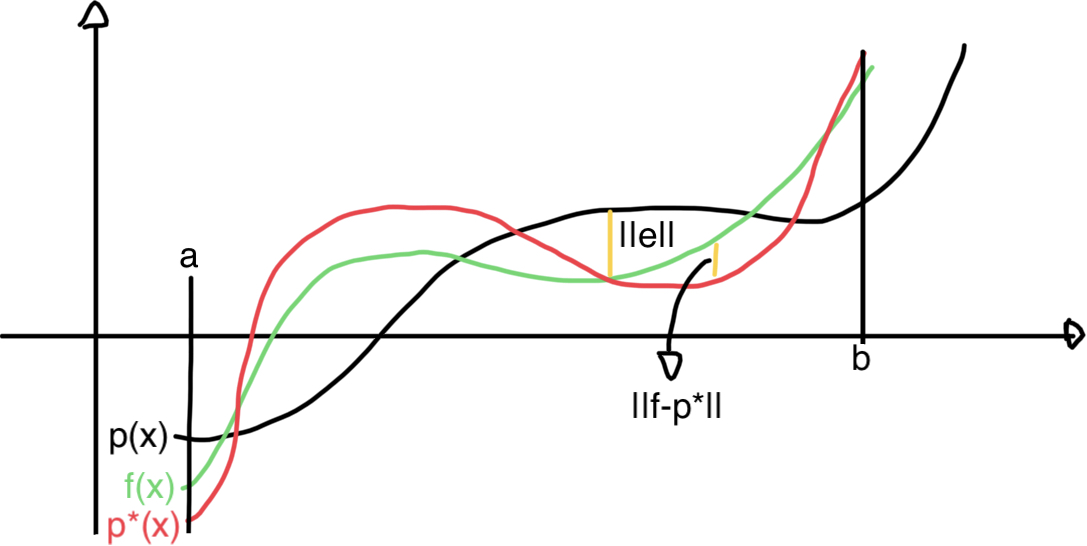
\includegraphics[width=0.75\textwidth]{immagini/esempioGrafMiglApprox.jpg}
    \caption{Esempio grafico della approssimazione $p$ e dell'errore (\ref{eq:errMiglAppross}) conseguente.}\label{fig:esempioGrafMiglApprox}
\end{figure}

Dato $p(x)$, polinomio interpolante $f(x)$ di grado $n$, è trattato come l'errore di interpolazione sia legato all'errore di migliore approssimazione (\ref{eq:errMiglAppross}). A questo scopo è definito $\boldsymbol{||e||=||f-p||}$, ovvero l'\textbf{errore massimo di interpolazione}.

\begin{theorem}\label{th:approxErrMiglApprox}\footnote{Slide 8 PDF 20, Teorema 4.7 PG 90}
    Sia $p*(x)$ il polinomio di migliore approssimazione di grado $n$ di $f(x)$, allora, per l'errore di interpolazione (\ref{eq:defErrInter}), vale:
    \begin{equation}\label{eq:errInterpMiglApprox}
        ||e||\leq (1+\boldsymbol{\Lambda_n})\overbrace{||f-p^*||}^{\footnotemark},
    \end{equation}
    dove $\boldsymbol{\Lambda_n}$ è la costante di Lebesque, definita sulle ascisse di interpolazione.
\end{theorem}\footnotetext{Quantità che tende a 0 quando $n$ cresce (lentamente in generale).}
\begin{proof}
Considerando $p^*\in\Pi_n$:
    \begin{equation*}
        \begin{matrix}
            ||e||&\overset{\footnotemark}{=}&||f-p^*+p^*-p||\\
            &\leq& ||f-p^*||+||p^*-p||\\
            &\leq& ||f-p^*||+\Lambda_n||f-p^*||
            &=&(1+\Lambda_n)||f-p^*||.
        \end{matrix}
    \end{equation*}\footnotetext{Aggiunto il polinomio $p^*$ per il quale vale la diseguaglianza triangolare.}
    Su $p^*(x)$ sono possibili le seguenti considerazioni:
    \begin{itemize}
        \item coincide con il suo polinomio interpolante sulle $n+1$ ascisse sul quale è definito $p(x)$;
        \item può essere interpretato come una perturbazione $\widehat f(x)$ di $f(x)$.
    \end{itemize}
\end{proof}

È necessaria un'approssimazione dell'errore di migliore approssimazione (\ref{eq:errMiglAppross}) in quanto l'errore crescerà al crescere di $n$, se la costante di Lebesque diverge esponenzialmente. Per questo è fornita una maggiorazione per (\ref{eq:errMiglAppross}), introducendo il modulo di continuità di una funzione.

\begin{definition}[Modulo di continuità di una funzione]
    Data $f\in C^{(0)}[a,b]$ è definito il modulo di continuità di $f$, per $h>0$ (variazione), come:
    \begin{equation}\label{eq:modCont}
        \boldsymbol{\omega(f;h)}=\left\{\underset{x,y\in [a,b]}{\sup}|f(x)-f(y)|:\; |x-y|\leq h\right\}.
    \end{equation}
\end{definition}

\begin{figure}
    \centering
    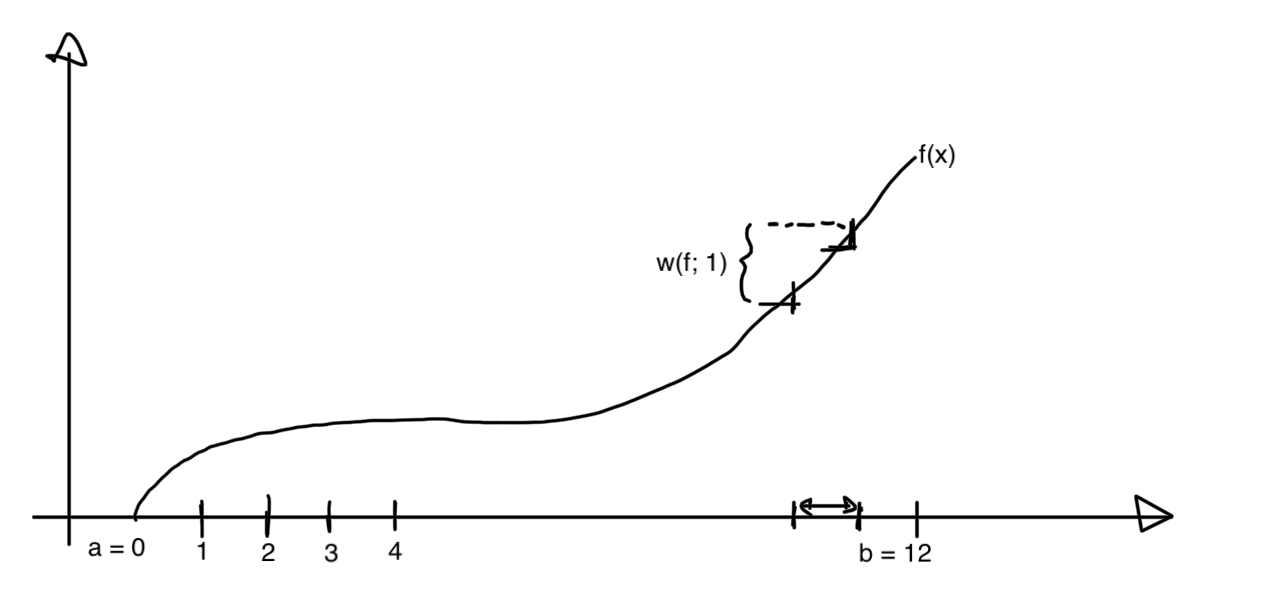
\includegraphics[width=0.75\textwidth]{immagini/modContEs.png}
    \caption{Esempio modulo di continuità. $\omega (f;1)$ è la massima distanza sul grafico di $f$ tra i punti.}\label{fig:modContEs}
\end{figure}

\begin{theorem}\label{th:modContInf}\footnote{Slide 10 PDF 20, primo punto PG 91}
    Se $f\in C^{(0)}[a,b]\Rightarrow\omega (f;h)\rightarrow 0$, per $h\rightarrow 0$.
\end{theorem}

\begin{definition}[Polinomio di migliore approssimazione]
    Data $f\in C^{(0)}[a,b]$ allora è definito polinomio di migliore approssimazione di grado $n$ di $f$ su $[a,b]$:
    \begin{equation}
        p^* \overset{\footnotemark}{=} \underset{p\in\Pi_n}{\arg\min}||f-p||.
    \end{equation}
\end{definition}

\footnotetext{$\underset{x\in X}{\arg\min}f(x)=\{x\,|\,\forall y : f(y)\geq f(x)\}$. In altre parole, è l'insieme dei valori di $x$ per i quali $f(x)$ raggiunge il suo più alto valore $M$.}

Dato $p(x)\in\Pi_n$, ovvero un polinomio interpolante $f(x)$ su $n+1$ ascisse in $[a,b]$, valgono i due seguenti risultati.

\begin{theorem}[Jackson]\label{th:Jackson}\footnote{Slide 10 PDF 20, Teorema 4.8 PG 91}
    Se $f\in C^{(0)}[a,b]$ e $p^*$ è il suo polinomio di migliore approssimazione di grado $n$, allora $\exists\, \alpha$, indipendente da $n$, tale che:
    \begin{equation}\label{eq:approxJackson}
        ||f-p^*||\leq \alpha\cdot\omega\left(f;\frac{\overset{\footnotemark}{b-a}}{\underset{\footnotemark}{n}}\right).
    \end{equation}
\end{theorem}

\addtocounter{footnote}{-1}
\footnotetext{Ampiezza dell'intervallo sul quale approssimiamo $f$.}

\stepcounter{footnote}
\footnotetext{Grado del polinomio di migliore approssimazione. Più questo cresce più $\omega\rightarrow 0$, quindi $||f-p||>0$.}

\begin{corollary}
    Se $f\in C^{(0)}[a,b]$, allora
    \begin{equation*}
        ||f-p^*_n||\rightarrow 0,\quad n\rightarrow\infty,
    \end{equation*}
    essendo $\{p^*_n\}$ la successione dei problemi di migliore approssimazione di $f$ di grado $n$.
\end{corollary}


È possibile affermare che esiste una relazione fra l'errore nell'approssimazione polinomiale ed il condizionamento del problema (dato il Teorema di Jackson).

\begin{corollary}\footnote{Slide 10 PDF 20, PG 91. Dalle (\ref{eq:errInterpMiglApprox})-(\ref{eq:approxJackson}) vale quanto segue.}
    $\forall n\geq 0$, data una funzione $f(x)$ generica, $p(x)$ il polinomio interpolante di grado $n$ su $n+1$ ascisse assegnate e $\Lambda_n$ la corrispondente costante di Lebesque, vale che:
    \begin{equation}\label{eq:maggErrMiglAprrox}
        \boxed{||e||=||f-p||\leq\underset{\footnotemark}{\alpha}\underbrace{(1+\Lambda_n)\,\omega\left(f;\frac{b-a}{n}\right)}_{\footnotemark}}.
    \end{equation}
\end{corollary}

\addtocounter{footnote}{-1}
\footnotetext{Non dipende da $n$, ovvero il grado del polinomio approssimante.}

\stepcounter{footnote}
\footnotetext{Definita nella dimostrazione del Teorema \ref{th:approxErrMiglApprox}.}

Quest'utlima espressione sarà utile per introdurre nuovi metodi di interpolazione. Inoltre, è necessario che la costante $\Lambda_n$ non cresca più rapidamente della quantità per la quale è moltiplicata, ma tenda a 0, al crescere del numero di ascisse di interpolazione.

\begin{remark}\footnote{Slide 10 PDF 20.}
    Al crescere del numero delle ascisse di interpolazione $(n+1)$ è necessario fare in modo che $\Lambda_n$ cresca in modo ottimale, affinché $||e||$ diminuisca.
\end{remark}

\subsection{Ascisse di Chebyshev}\label{ssec:AscCheb}\footnote{PDF 21, PG 91-93.}
Le Sezioni \ref{ssec:errInter} e \ref{ssec:condProbApproxfun} sono riassumibili nei seguenti punti:
\begin{itemize}
    \item $\Lambda_n$ è indipendente dal particolare intervallo considerato; cresce esponenzialmente con $n$ se sono utilizzate ascisse equidistanti, altrimenti ha una crescita moderta (quella ottimale è di tipo logaritmico) rispetto ad $n$; \footnote{$n$ è il grado del polinomio interpolante.}
    \item Data la maggiorazione $||e||\leq \frac{\overbrace{||f^{(n+1)}||}^{\footnotemark}}{(n+1)!}||\omega_{n+1}||,\text{ con } \omega_{n+1}(x)=\prod_{j=0}^n(x-x_j)$, è necessario capire come questa sia collegata con (\ref{eq:maggErrMiglAprrox}). 
\end{itemize}\footnotetext{Indipendente dalle ascisse, non come $||w_{n+1}||$.}

L'obbiettivo della Sezione è  quello di scegliere le ascisse di interpolazione $x_j$ in modo da minimizzare $||\omega_{n+1}||$. Per fare questo è necessario rendere la costante di Lebesque piccola o almeno con una precisione accettabile.

Considerando l'intervallo di riferimento $\boldsymbol{[-1,1]}$, è necessario scegliere le ascisse $x_0,\hdots,x_n$ in modo tale da risolvere il problema del \textbf{minmax}, ovvero il seguente: \footnotemark
\begin{equation}\label{eq:minmax}
    \underset{a=-1\leq x_0<\hdots<x_n\leq 1=b}{\min}||w_{n+1}||=\boldsymbol{\underset{a=-1\leq x_0<\hdots<x_n\leq 1=b}{\min}\quad\underset{-1\leq x\leq 1}{\max}|}\overbrace{\boldsymbol{w_{n+1}(x)}}^{\footnotemark}\boldsymbol|,
\end{equation}
con $w_{n+1}(x)$ calcolata come in (\ref{polBaseNewt2}), ovvero $\prod_{j=0}^n(x-x_j)$.
\addtocounter{footnote}{-1}
\footnotetext{Slide 5 PDF 21, PG 91.}

\stepcounter{footnote}
\footnotetext{Polinomio monico che ha come radici le ascisse, rispetto alle quali è svolta la minimizzazione.}

A questo scopo è introdotta la seguente Definizione:

\begin{definition}[Polinomi di Chebyshev di I specie]\label{th:polChebIsp}
    Assunto $x\in [-1,1]$, la \textbf{famiglia di polinomi di Chebyshev di I specie} è definita come segue:
    \begin{equation}\label{eq:polChebISp}
        \begin{cases}
        T_0(x) \equiv 1;\\
        T_1(x) = x;\\
        T_{k+1}(x) = 2x\cdot T_k(x)-T_{k-1}(x),\;\; k\geq 1.
        \end{cases}
    \end{equation}
\end{definition}

\begin{example}
    \begin{equation*}
        \begin{matrix}
            T_2 &=& 2x \cdot \equaltoup{x}{T_1(x)} - \equaltoup{1}{T_0(x)} &=& 2x^2-1,\\
            T_3(x) &=& 2x\cdot T_2(x)-T_1(x)&=&2x(2x^2-1)-x&=& 4x^3-2x-x &=& 4x^3-3x,\\
            \vdots
        \end{matrix}
    \end{equation*}
    \qed
\end{example}

Alcune proprietà dei polinomi di Chebyshev di I specie sono le seguenti:
\begin{itemize}
    \item [P1)] $\boldsymbol{T_k(x)}$ è un \textbf{polinomio di grado esatto} $\boldsymbol k,\,\forall k=0,1,\hdots$;
    \item[P2)]\footnotemark Il coefficiente principale di $\boldsymbol{T_k(x)}$ è $\boldsymbol{2^{k-1}},\,\forall\,k=1,2,\hdots$;
    \footnotetext{A cosa serve questa proprietà? Dato il polinomio $4x^2-1$, è necessario dividerlo per 4 per renderlo monico (4 è il coeficiente principale del polinomio). Data una famiglia di polinomi di grado $k$, se è necessario derivare una famiglia di polinomi monici è necessario conoscere qual è il coefficiente principale di ciascuno di loro.}
    \item[P3)]\footnotemark I polinomi $\boldsymbol{\left\{\widehat T_k\right\}_{k\geq 0}}$ definiti come
    \begin{equation*}
        \begin{cases}
            \widehat T_0(x)=T_0\equiv 1,\\
            \widehat T_k(x) =\boldsymbol{2^{1-k}}\, T_k(x),\;\; k=1,2,\hdots
        \end{cases}
    \end{equation*}
    sono una \textbf{famiglia di polinomi monici} (perché $2^{1-k}$ è il reciproco del precedente coefficiente $2^{k-1}$);
    \footnotetext{Dati i polinomi di grado $k$ con 8 coefficienti principali, è possibile derivare da questa una famiglia di polinomi monici.}
    \item[P4)] 
    \begin{equation*}
        \forall\, k\geq 1: \widehat T_k(x)=\prod_{j=0}^{k-1}\left(x-x_j^{(k)}\right),
    \end{equation*}
    con $T_k\left(\boldsymbol{x_j^{(k)}}\right)=0,\; j=0,\hdots,k-1,\;\text{dove } \boldsymbol{x_j^{(k)}}$ sono le \textbf{radici} di $\boldsymbol{T_k(x)}$. \footnote{Se le radici $x_j^{(k)}$ fossero tutte distinte e nell'intervallo $[-1,1]$, allora per il polinomio $\widehat T_k(x)$ è possibile scegliere un'ascissa di interpolazione.}
\end{itemize}

\begin{remark}\label{re:ver1&2}\footnote{Slide 7 PDF 21.}
    Considerata $\widehat T_{n+1}(x)=\prod_{j=0}^n\left(x-x_j^{(n+1)}\right)$, dove $x_j^{(n+1)},\; j=0,\hdots,n$, sono le radici di $T_{n+1}(x)$ e date le seguenti condizioni sulle radici:
    \begin{enumerate}
        \item $x_i^{(n+1)}\neq x_j^{(n+1)},\quad i\neq j,\; i,j=0,\hdots,n;$ \footnote{Definisce le ascisse distinte.}
        \item $x_j^{(n+1)}\in [-1,1],\quad \forall j=0,\hdots,n;$ \footnote{Definisce le ascisse in un intervallo.}
    \end{enumerate}
    allora è possibile sceglierle come ascisse di interpolazione, per cui:
    \begin{equation*}
        \boldsymbol{\omega_{n+1}\equiv\widehat T_{n+1}=\prod_{j=0}^{n}\left(x-x_j^{(n+1)}\right)}.
    \end{equation*}
    Per verificare che 1. e 2. siano soddisfatte, sarà ottenuta un'espressione esplicita delle ascisse stesse. Poiché $x\in [-1,1]$, è posto $x=\cos(\theta),\, \theta\in [0,\pi],$ allora $\theta=\arccos{x}$ (vedere Figura \ref{fig:cosThetaChebyshev}).
\end{remark}

\begin{figure}
    \centering
    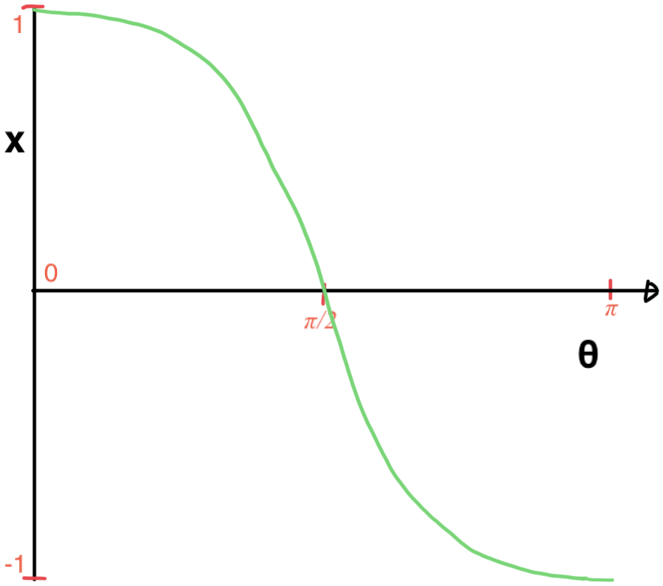
\includegraphics[width=0.35\textwidth]{immagini/cosThetaChebyshev.png}
    \caption{Grafico osservazione \ref{re:ver1&2}.}\label{fig:cosThetaChebyshev}
\end{figure}

\begin{itemize}
    \item[P5)] Se $\boldsymbol{x=\cos\theta}\Rightarrow T_k(x)=T_k(\cos\theta)=\cos{k\theta}\;\footnotemark.$
    \footnotetext{Polinomio di Chebyschev, se $x$ è parametrizzata in modo idoneo.}
    \begin{proof}
        È svolta per induzione su $k$.
        \begin{equation*}
            \begin{matrix}
                k=0&\Rightarrow& T_0(x) &=& T_0(\cos\theta) &=& \cos{(0\cdot\theta)} &\equiv& 1,\\
                k=1 &\Rightarrow& T_1(x) &=& T_1(\cos\theta) &=& \cos\theta &=& x,
            \end{matrix}
        \end{equation*}
        supposto vero per $k$ e $k-1$ è dimostrato per $k+1$ ciò che segue:
        \begin{equation*}
            \begin{matrix}
                \boldsymbol{T_{k+1}(x)}&\boldsymbol =& 2x\,T_k(x)-T_{k-1}(x) &=& 2cos\theta\cdot\cos{(k\theta)}-\cos{((k-1)\theta)}\\
                &=&2cos\theta\cdot\cos{(k\theta)}-\cos\theta\cdot\cos{(k\theta)}-\sin\theta\sin{(k\theta)} &=& \cos\theta\cdot\cos{(k\theta)}-\sin\theta\cdot\sin{(k\theta)}\\
                &&&=&\boldsymbol{\cos{((k+1)\,\theta)}}
            \end{matrix}
        \end{equation*}
    \end{proof}
    \item[P6)]\footnotemark $||T_k||=\underset{\theta\in [0,\pi]}{\max}|\cos{k\theta}|
    \underset{\footnotemark}{=} 1,\;\forall k\geq 0$;
    \addtocounter{footnote}{-1}
    \footnotetext{Deriva dalla precedente proprietà.}
    \stepcounter{footnote}
    \footnotetext{In $[0,\pi]$ il massimo vale 1.}
    \item[P7)]$||\widehat T_k||=2^{1-k}||T_k||=2^{1-k},\;\forall k\geq 1$, con $\widehat T_k$ detto polinomio monicizzato;
    \item[P8)] Gli zeri di $T_k(x)$ sono ottenuti imponendo che $x=\cos\theta,\;\theta\in [0,\pi]$ e 
    \begin{equation*}
        \begin{matrix}
            T_k(x)&=&T_k(\cos\theta)=\cos{(k\theta)}=0\\
            &\underset{\footnotemark}{\Rightarrow}& k\theta=\frac{\pi}{2}+i\,\pi\\
            &\Rightarrow&\theta =\frac{(2i+1)\pi}{2k},\, \boldsymbol{i=0,\hdots,k-1}\\
            &\Rightarrow& x_i^{(k)} = \cos{\left(\frac{2i+1}{2k}\pi\right)},\, i=0,\hdots,k-1.
        \end{matrix}
    \end{equation*}\footnotetext{$\cos{(k\theta)}$ si annulla per $k\theta$ come segue.}
    con le ascisse risultanti reali, distintinte tra loro e appartenenti a $(-1,1)$.
\end{itemize}

\begin{definition}[Ascisse di Chebyshev]\footnote{Slide 10 PDF 21, TH 4.9 PG 92.}
    Dato il polinomio interpolante $f$ di grado $n$, le ascisse di Chebyshev sono definite come
    \begin{equation}\label{eq:ascisseChebyshev}
        x_i=\cos{\left(\frac{(2i+1)\pi}{2(n+1)}\right)},\quad i=0,\hdots,n,
    \end{equation}
    le quali sono le radici di $\widehat T_{n+1}(x)$.
\end{definition}

Dato che le ascisse di Chebyshev, appena definite, sono radici di $\widehat T_{n+1}(x)$ allora la norma
\begin{equation*}
    ||\omega_{n+1}||=||\widehat T_{n+1}||=2^{-n}\,||T_{n+1}||=2^{-n}\, 1 = \boldsymbol{2^{-n}}
\end{equation*}
è \textbf{minima} tra tutti \textbf{polinomi monici di grado} $\boldsymbol{n+1}$.\footnote{Comunque siano date le ascisse in $[-1,1]$ è ottenuto un valore più grande del $\min\max$ (\ref{eq:minmax}).} Pertanto, il polinomio di Chebyshev monicizzato di grado $n+1$ è soluzione del prodotto $\min\max$ (\ref{eq:minmax}). 

Inoltre, con la scelta delle ascisse di Chebyshev come ascisse di interpolazione è minimizzata la maggiorazione dell'errore (\ref{eq:approxJackson}), portando la costante di Lebesque a $\boldsymbol{\Lambda_n\approx\frac{2}{\pi}\log n}$. Quindi, la scelta delle ascisse di Chebyshev permette una crescita \textbf{ottimale} della costante di Lebesque, per $\boldsymbol{n\rightarrow\infty}$.

%%\vspace{6px}
%\hrule
%\vspace{-7px}
\paragraph{Ricapitolando:} Sono scelte le ascisse di interpolazione, nell'intervallo $[-1,1]$, distinte fra loro e che utilizzano la norma del polinomio monico (il quale ha come radici le ascisse del tipo $x_i$ definite in (\ref{eq:ascisseChebyshev})). 

È stato dimostrato che $||w_{n+1}||=2^{-n}$, con $n$ ottenuto attraverso le ascisse di interpolazione e le ascisse del polinomio di Chebyshev di grado $n$. 

Le ascisse del polinomio di Chebyshev di grado $n+1$ ha $n+1$ radici (necessario che un polinomio di Chebyshev di grado $n+1$ abba $n+1$ radici); con $n+1$ ascisse di interpolazione è possibile definire il polinomio interpolante di grado $n$. Quindi, se è richiesta una function per calcolare le ascisse relative al grado $n$, è neceessario ricordare di contare fino ad $n+1$ per Matlab, altrimenti sono contati $n-1$ (quindi il polinomio interpolante sarebbe di grado $n-1$).

%\vspace{3px}
%\hrule
%\vspace{6px}

\begin{figure}
    \centering
    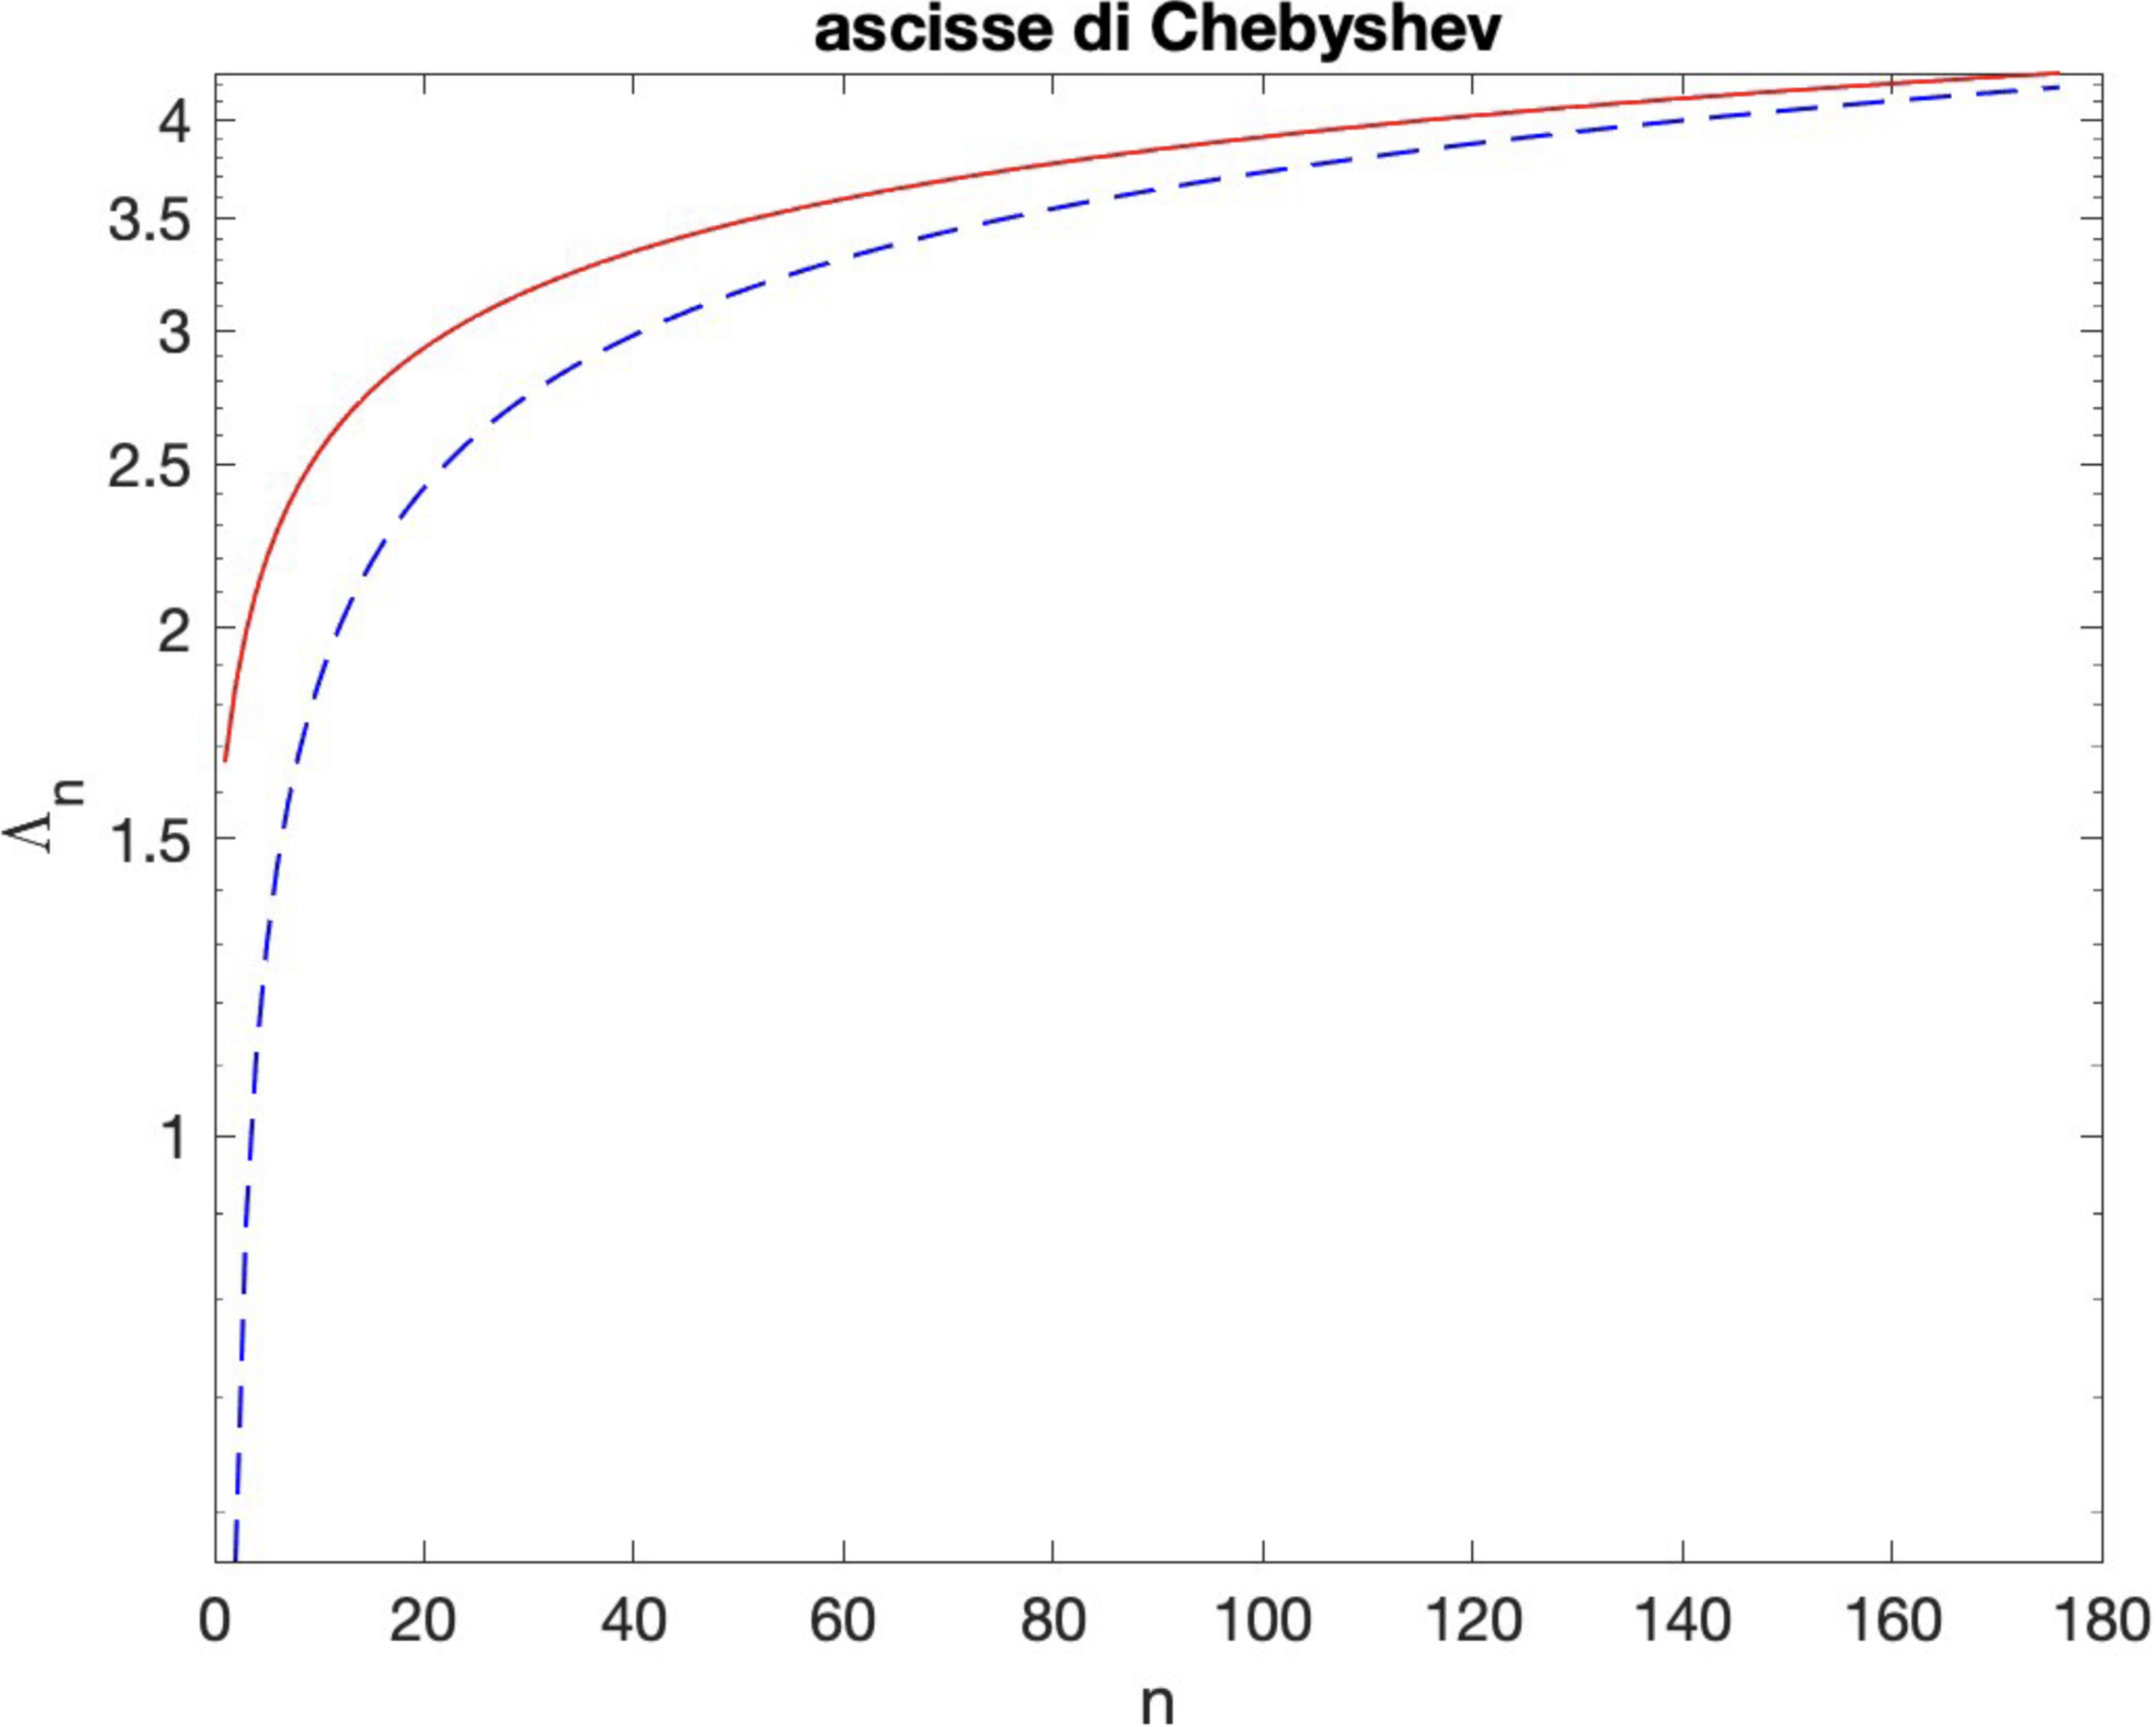
\includegraphics[width=0.5\textwidth]{immagini/graficoAscisseChebyshev.jpeg}
    \caption{Esempio di crescita di $\Lambda_n$ al crescere di $n$.}\label{fig:graficoAscisseChebyshev}
\end{figure}

Dalla Figura \ref{fig:graficoAscisseChebyshev} è possibile notare che sopra il grado 40 non vengono considerati i polinomi. Questo è dovuto al fatto che in aritmetica finita sono introdotti errori e molcondizionamento nelle operazioni. Inoltre, è introdotta la cancellazione numerica nel caso di differenza con ascisse di interpolazione sempre più vicine.

\begin{remark}
    Le ascisse di Chebyshev forniscono delle ascisse di interpolazione ottimali nell'intervallo $[-1,1]$. Per riportare ad un generico intervallo $[a,b]$ quanto descritto per (\ref{eq:ascisseChebyshev}), è possibile verificare facilmente che è sufficiente utilizzare la trasformazione lineare:
    \begin{equation*}
        x_{\boldsymbol{n-i}} =\underbrace{\frac{a+b}{2}}_{\footnotemark} + \frac{b-a}{2}\cos{\left(\frac{(2i+1)\pi}{2(\boldsymbol{n+1})}\right)},\quad i=0,\hdots,n,
    \end{equation*}
    dove è utilizzato l'indice di enumerazione in notazione $n-i$, quindi rovesciato, per ottenere le ascisse in ordine crescente. 
\end{remark}
\footnotetext{Punto medio dell'intervallo.}

Utilizzando le ascisse di Chebyshev nell'intervallo $[-5,5]$ sono ottenute le Figure \ref{fig:fRungeAscChebN=2}-\ref{fig:fRungeAscChebN=22}. Nelle figure è possibile notare che, da $n=10$ (vedere Figura \ref{fig:fRungeAscChebN=10}), la precisione di approssimazione è buona. Nella precedente approssimazione di $f(x)=\frac{1}{1+x^2}$ tramite la funzione di Runge, è possibile notare come, con 10 e più ascisse, erano presenti oscillazioni enormi agli estremi (vedere Figura \ref{fig:funzRunge_n=10} e \ref{fig:funzRunge_n=22}). Inoltre, è possibile notare come le ascisse addensate agli estremi dell'intervallo sono più vicine l'una alla altra di quanto lo siano quelle centrali.

È possibile trovare un'implementazione dell'algoritmo che calcola le ascisse di Chebyshev, per costruire il polinomio interpolante di grado $n$, su un generico intervallo $[a, b]$, nell'Algoritmo \ref{alg:cheby}.

\begin{remark}
    È necessario ricordare che al crescere del grado $n$ del polinomio interpolante, la scelta delle ascisse di interpolazione non deve fare crescere troppo la costante di Lebesque $\Lambda_n$.
\end{remark}

\begin{figure}
    \centering
    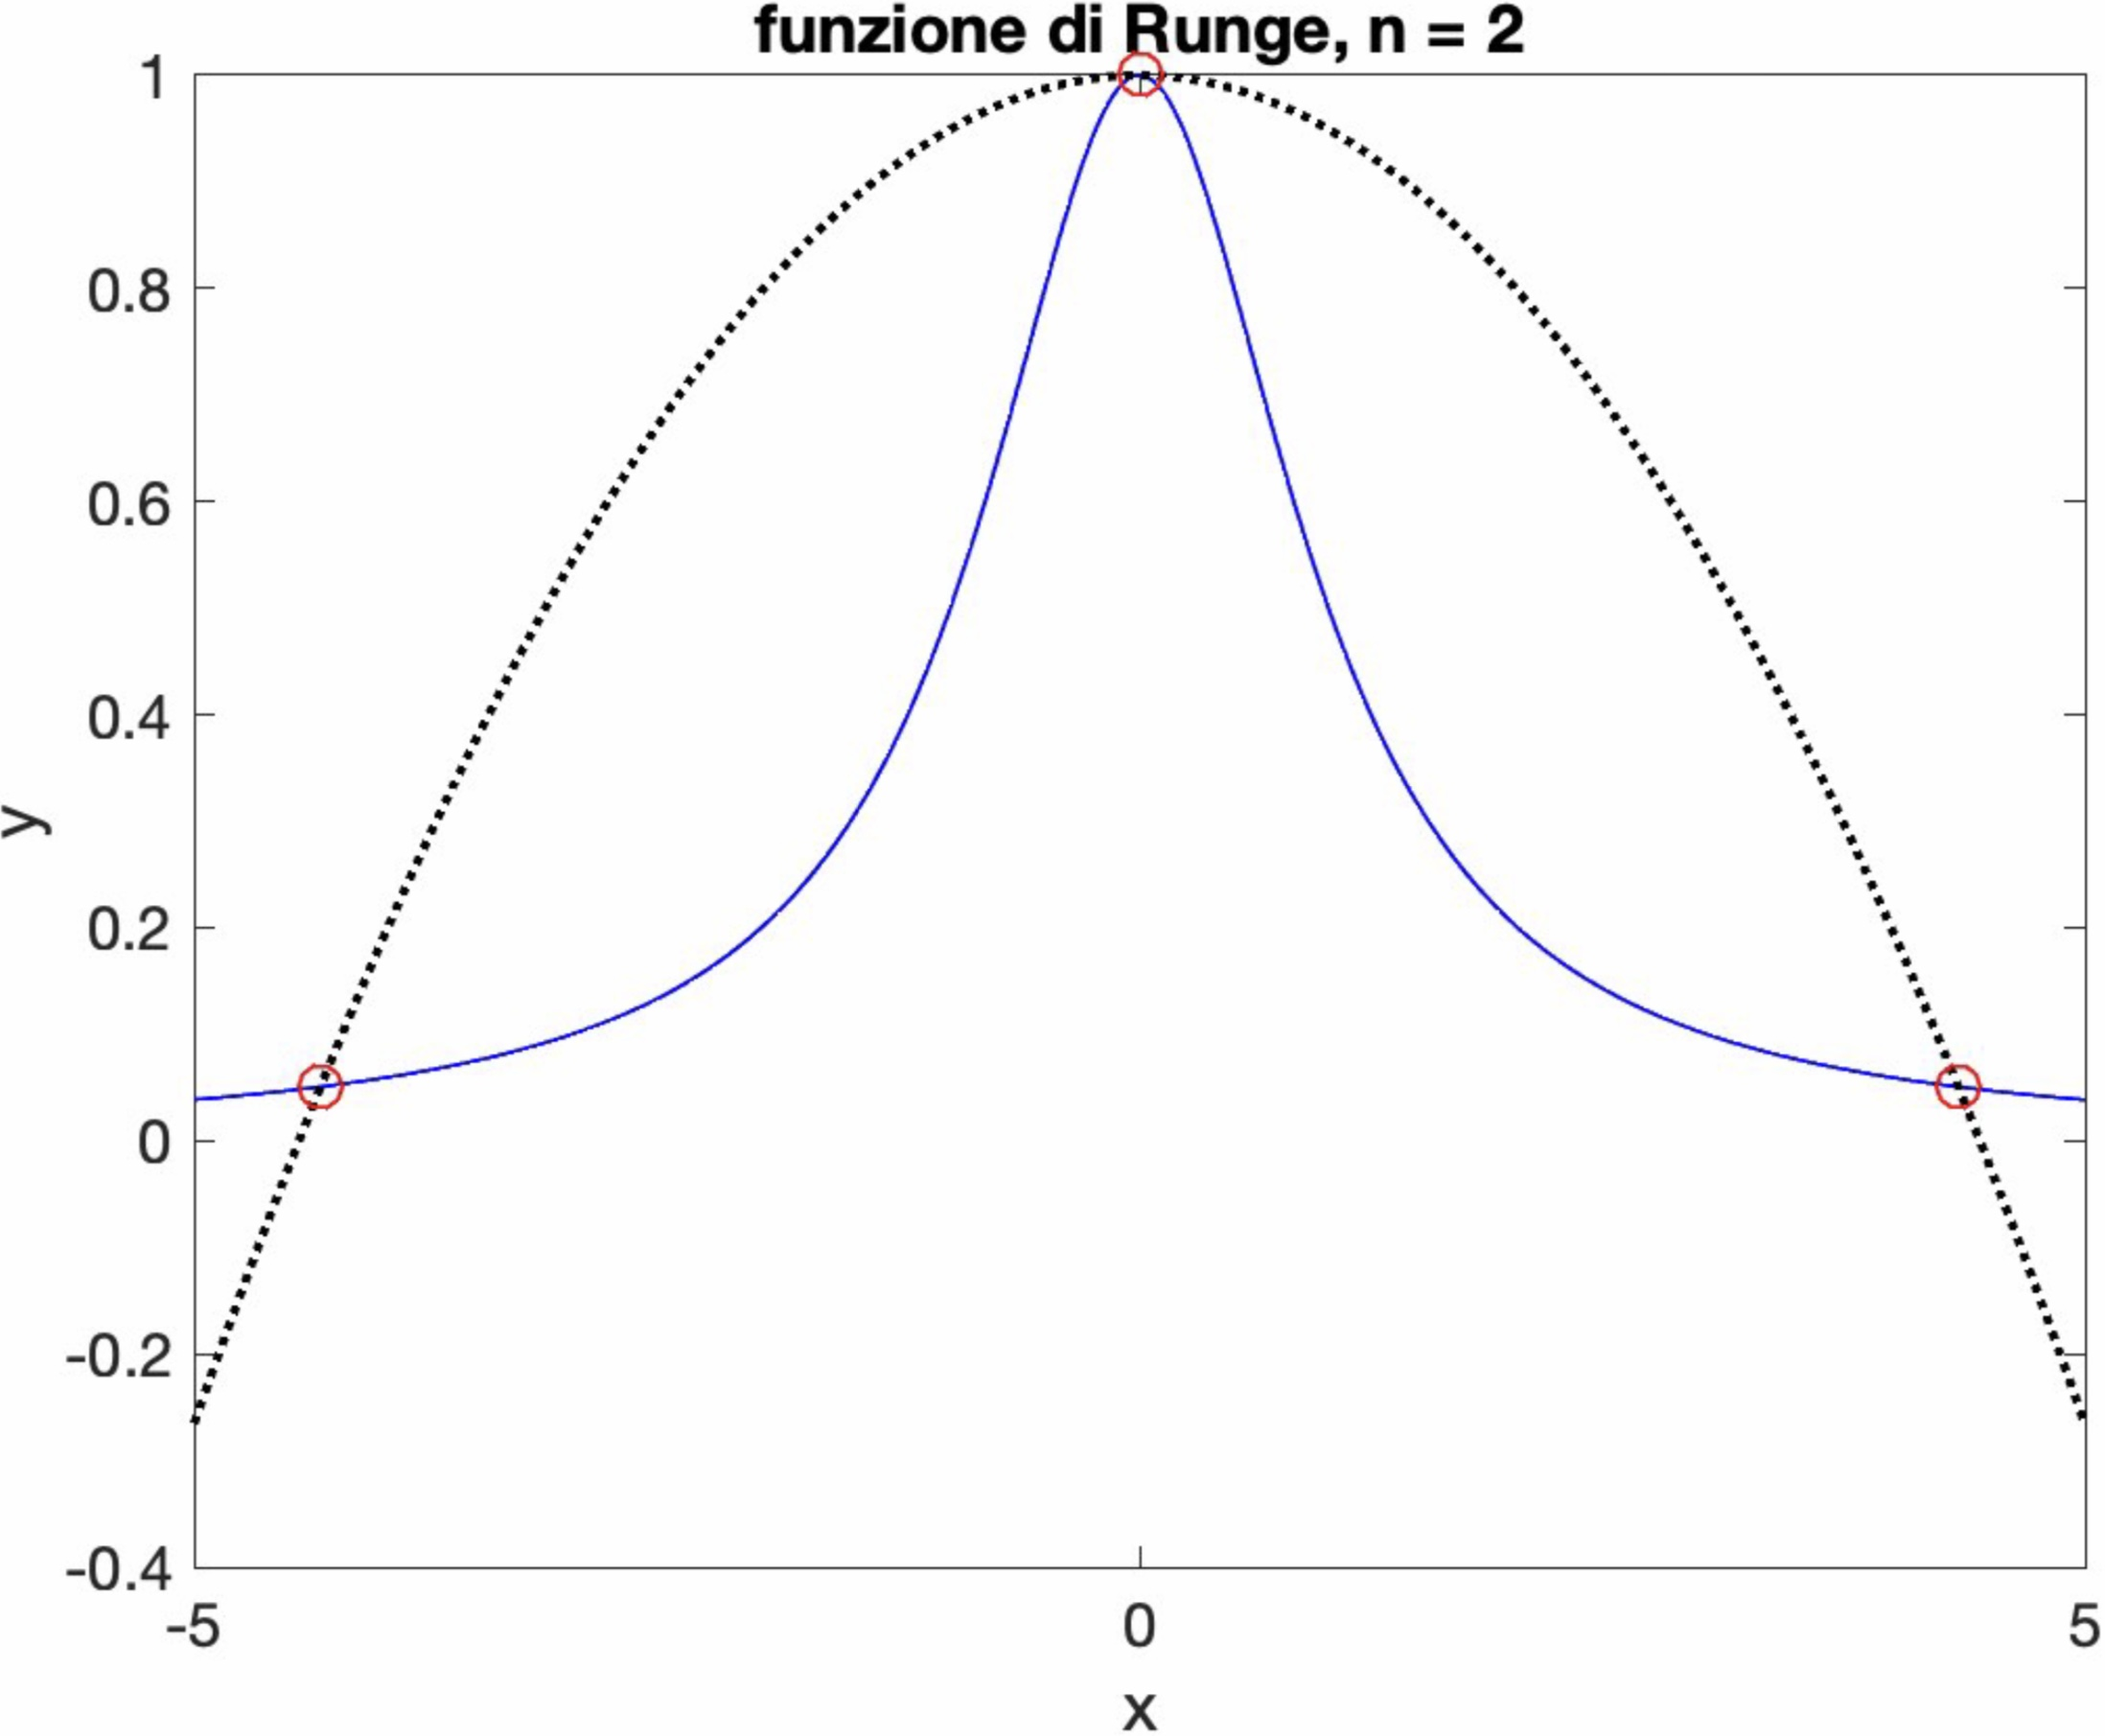
\includegraphics[width=0.5\textwidth]{immagini/fRungeAscChebN=2.jpg}
    \caption{Esempio di crescita di $\Lambda_n$ al crescere di $n$.}\label{fig:fRungeAscChebN=2}
\end{figure}

\begin{figure}
    \centering
    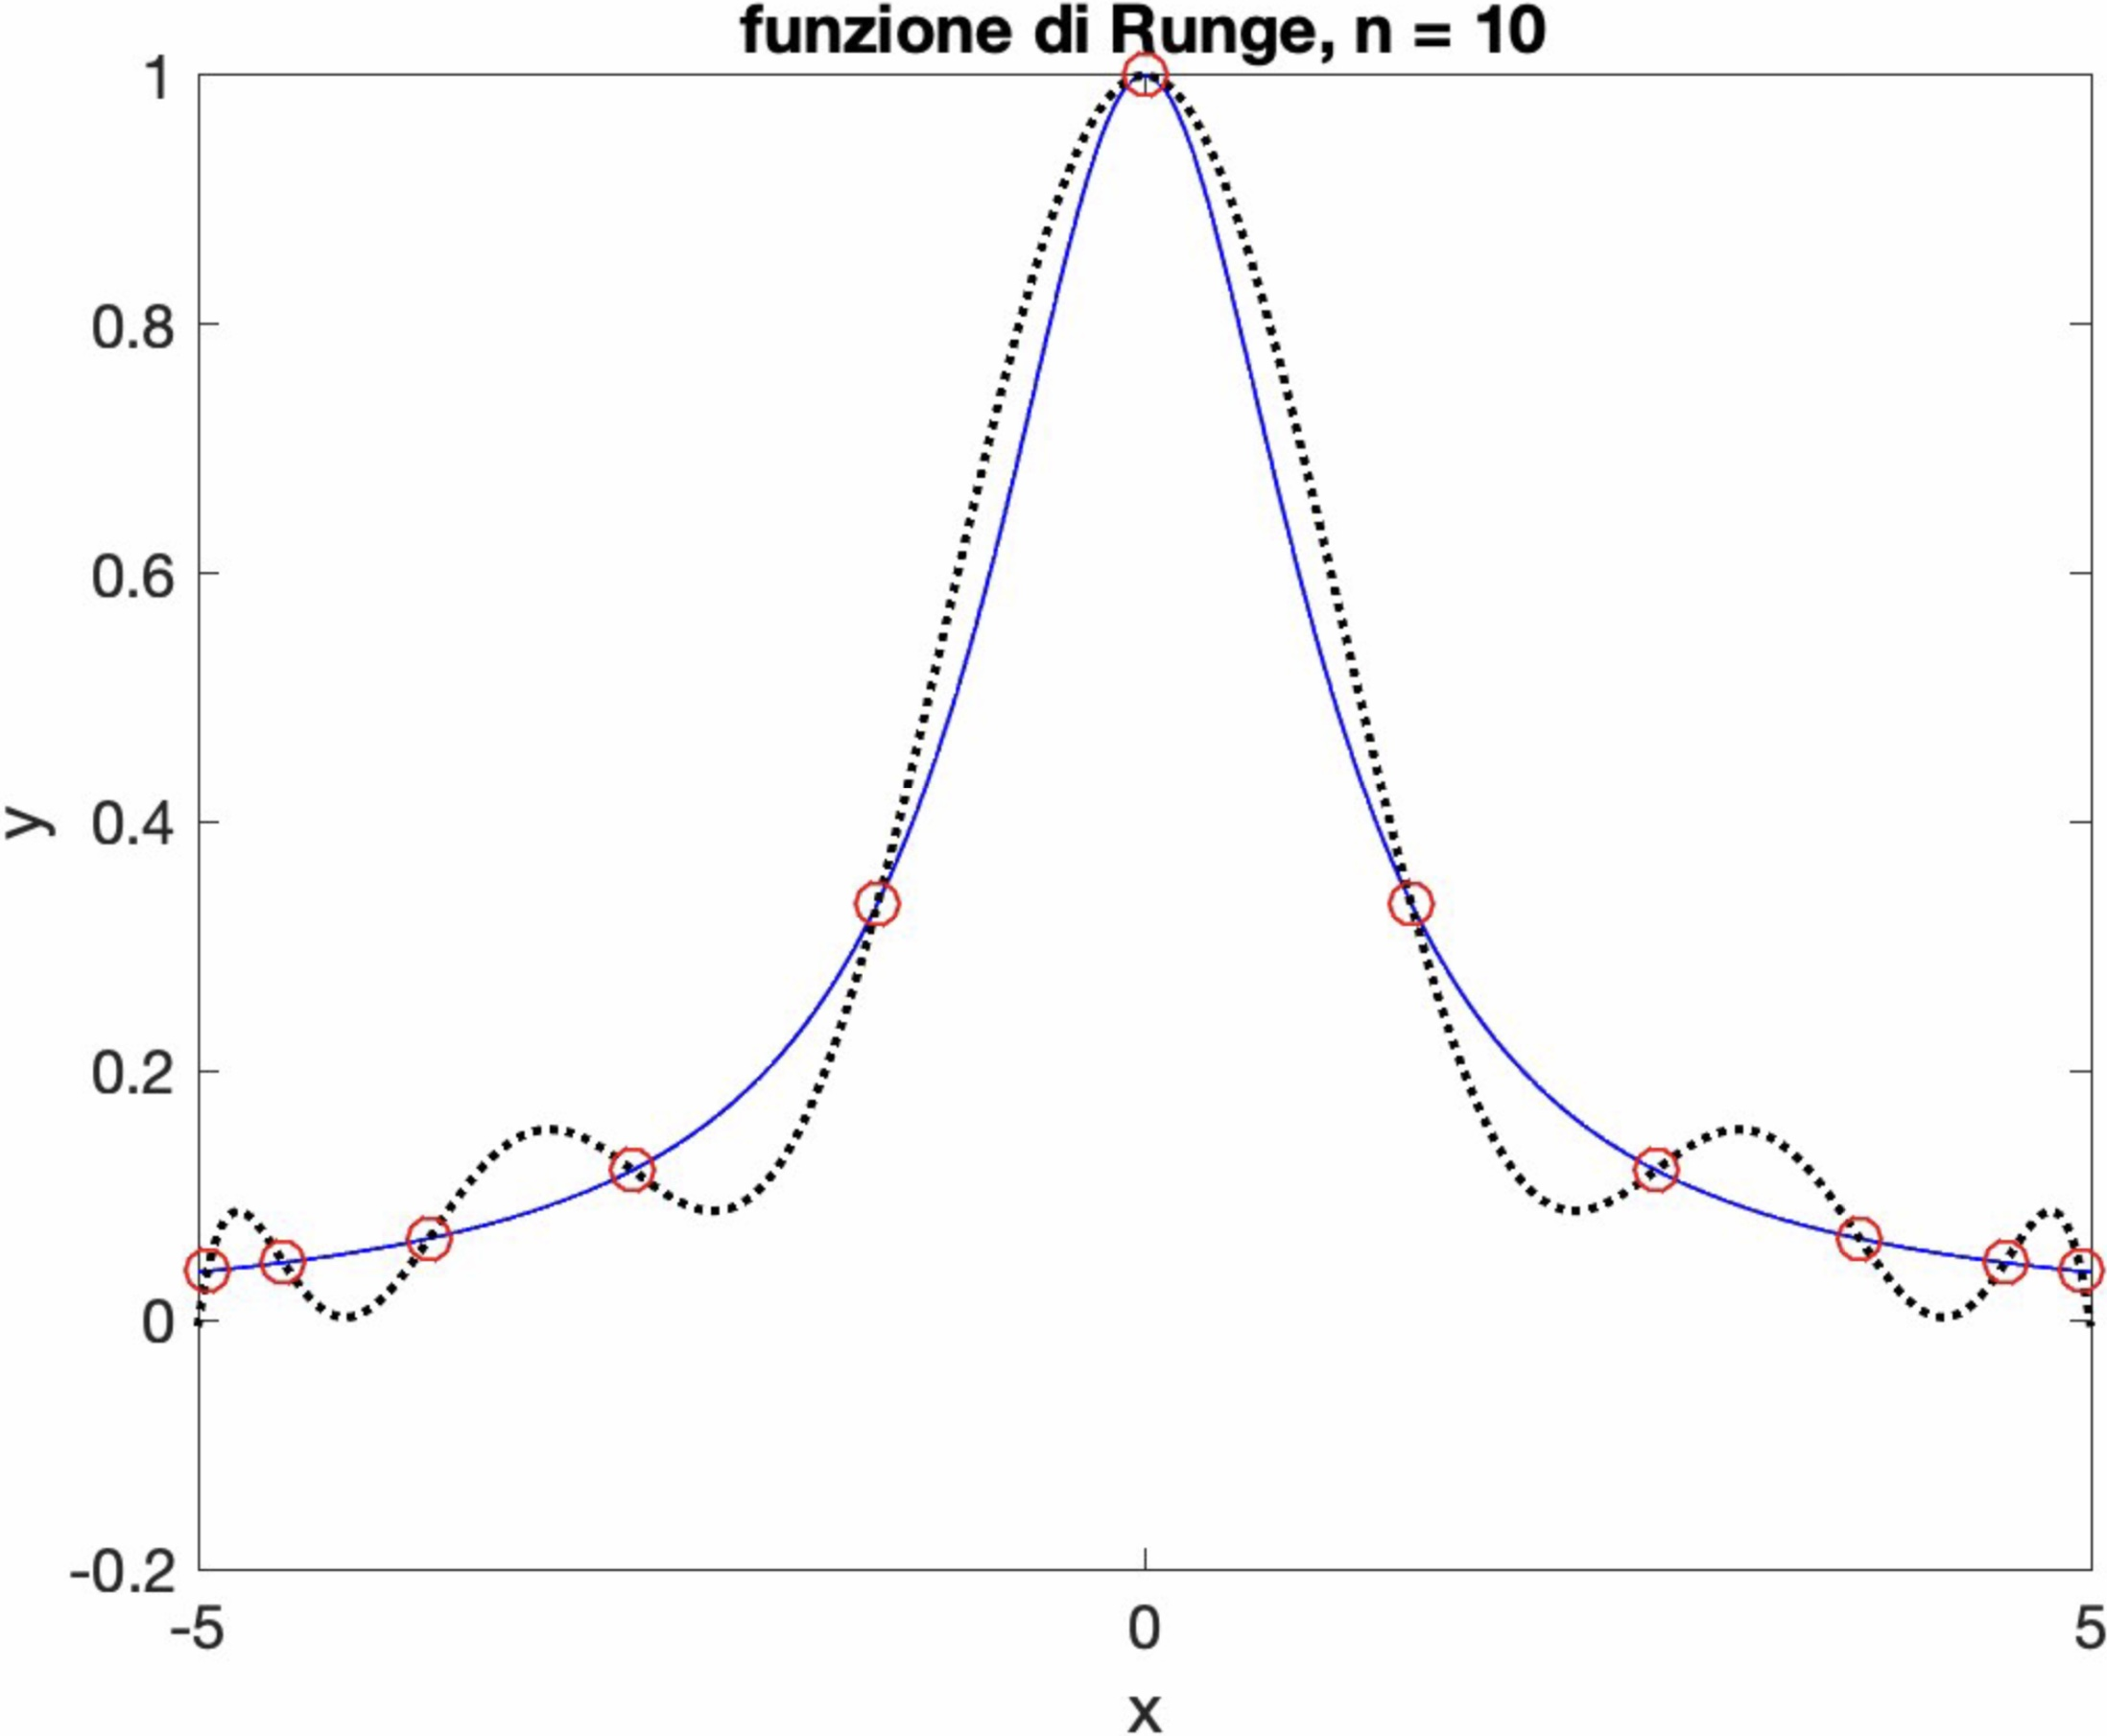
\includegraphics[width=0.5\textwidth]{immagini/fRungeAscChebN=10.jpg}
    \caption{Esempio di crescita di $\Lambda_n$ al crescere di $n$.}\label{fig:fRungeAscChebN=10}
\end{figure}

\begin{figure}
    \centering
    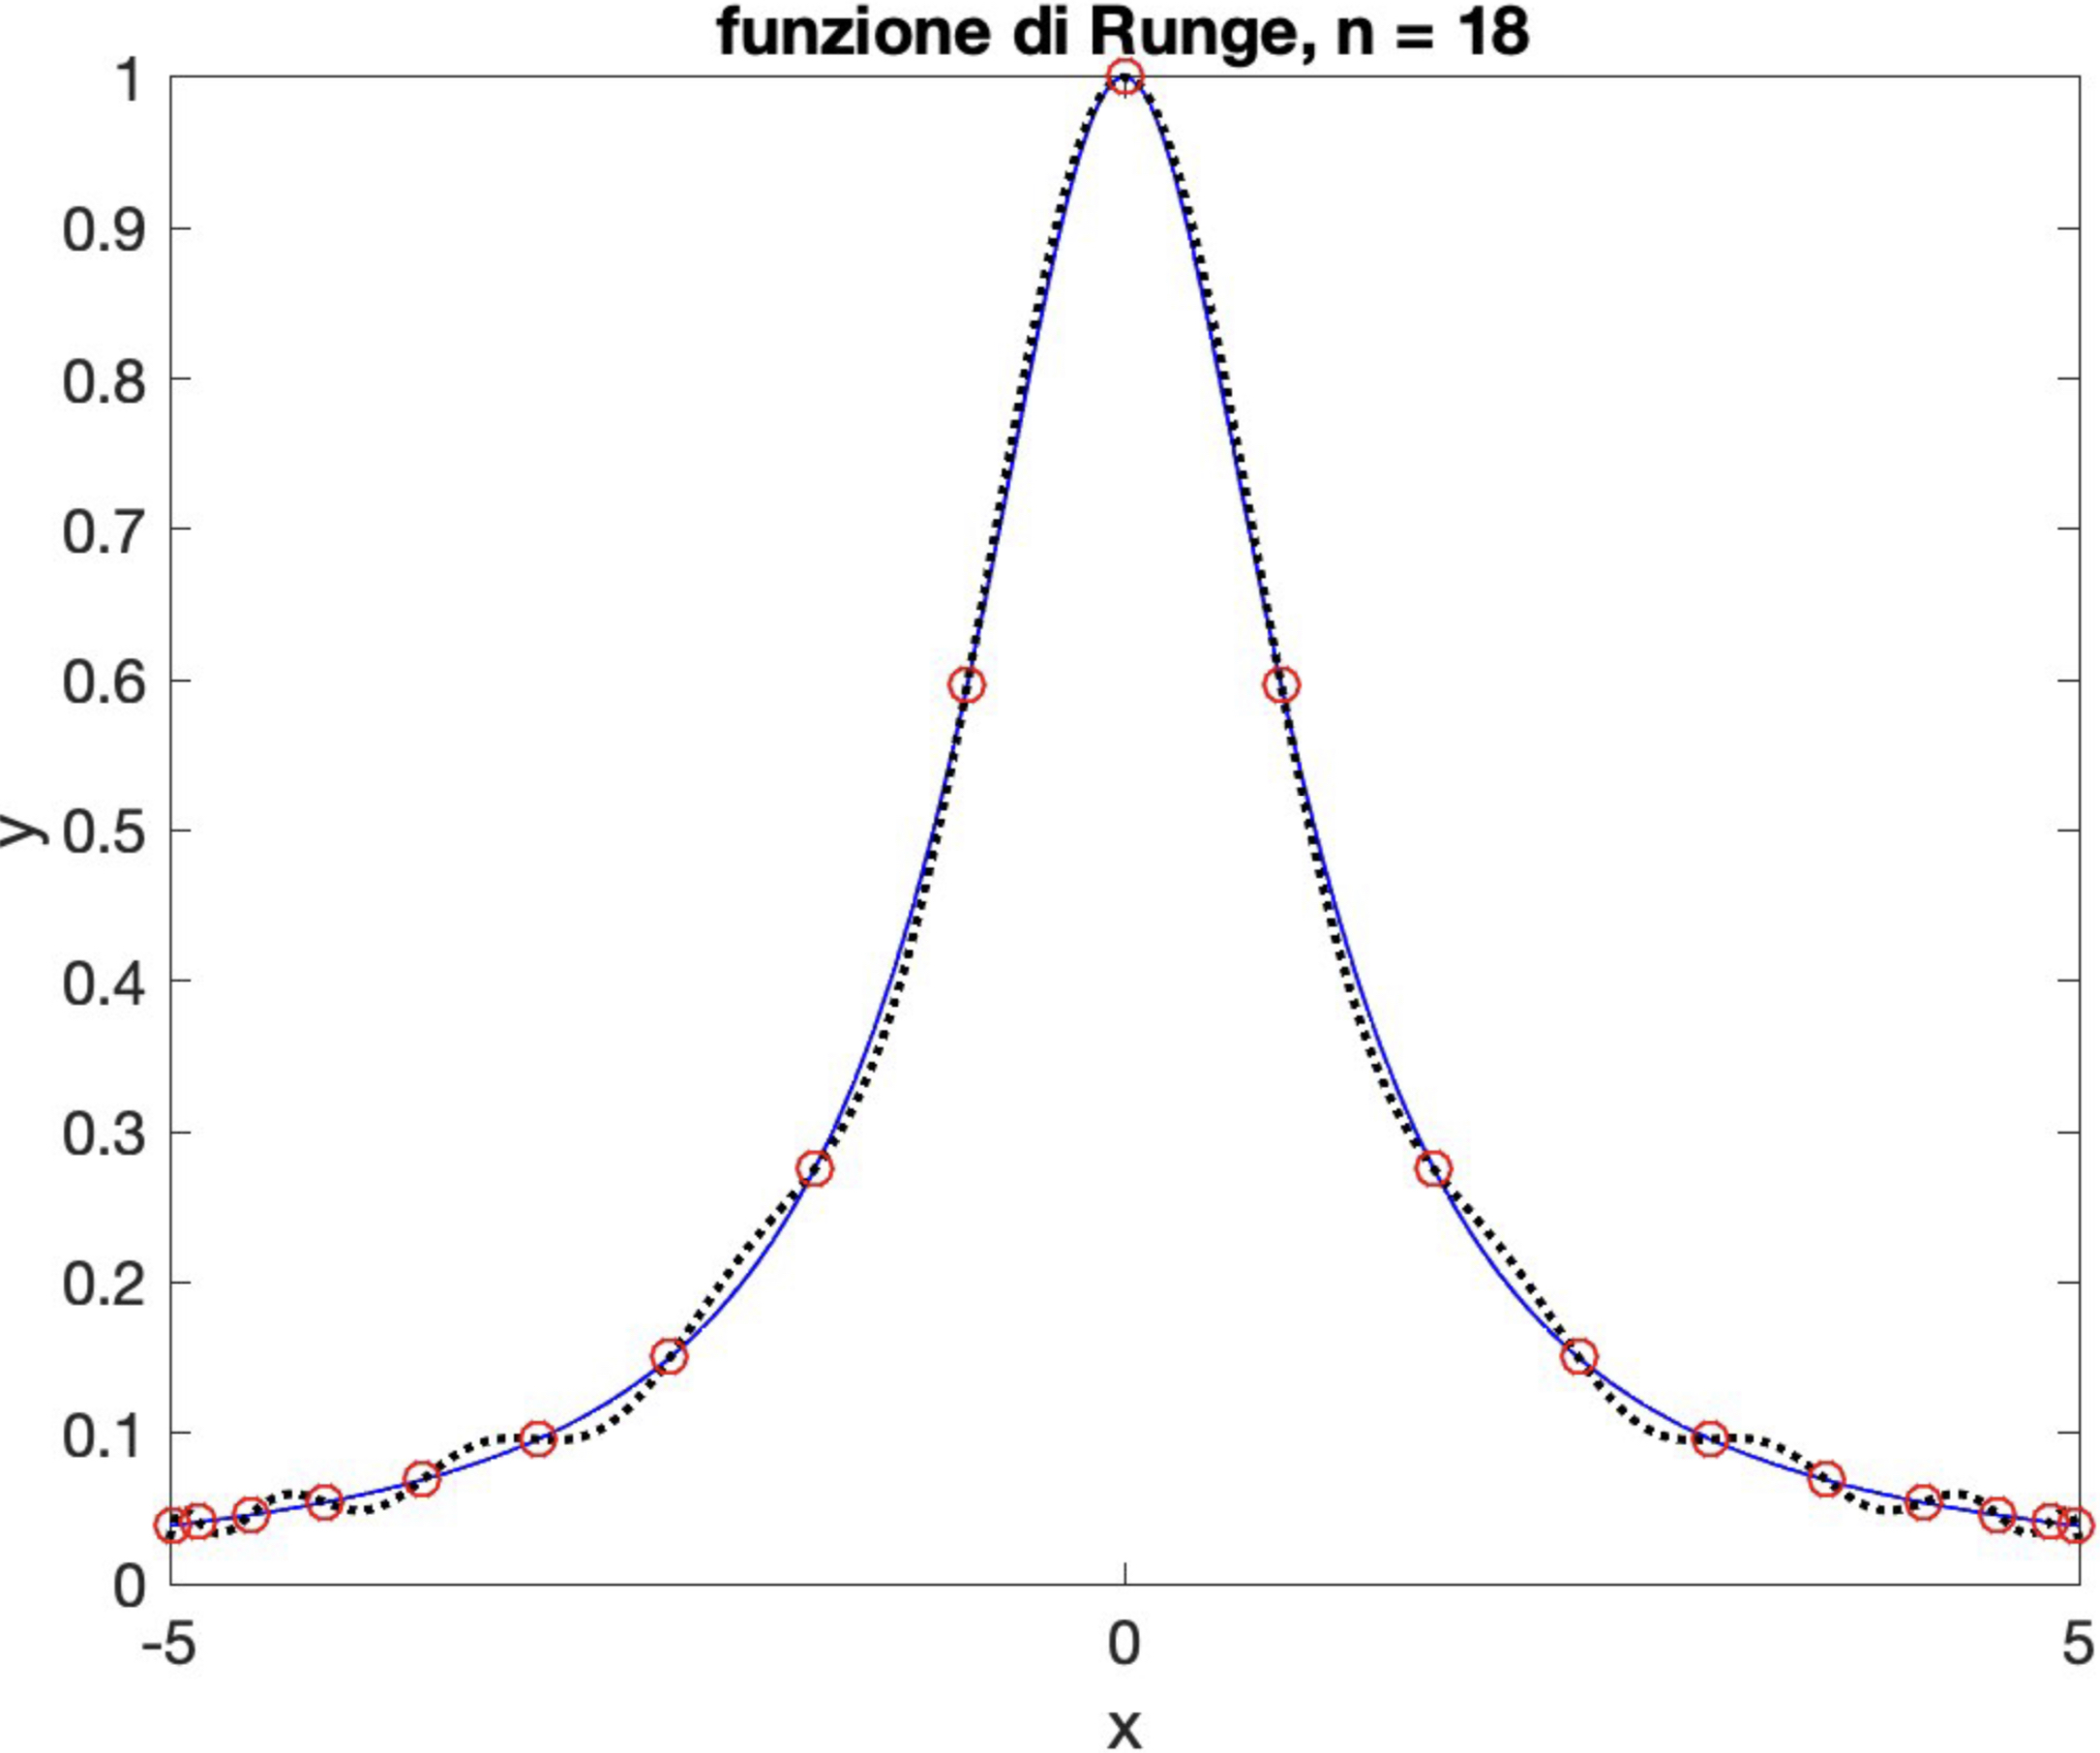
\includegraphics[width=0.5\textwidth]{immagini/fRungeAscChebN=18.jpg}
    \caption{Esempio di crescita di $\Lambda_n$ al crescere di $n$.}\label{fig:fRungeAscChebN=18}
\end{figure}

\begin{figure}
    \centering
    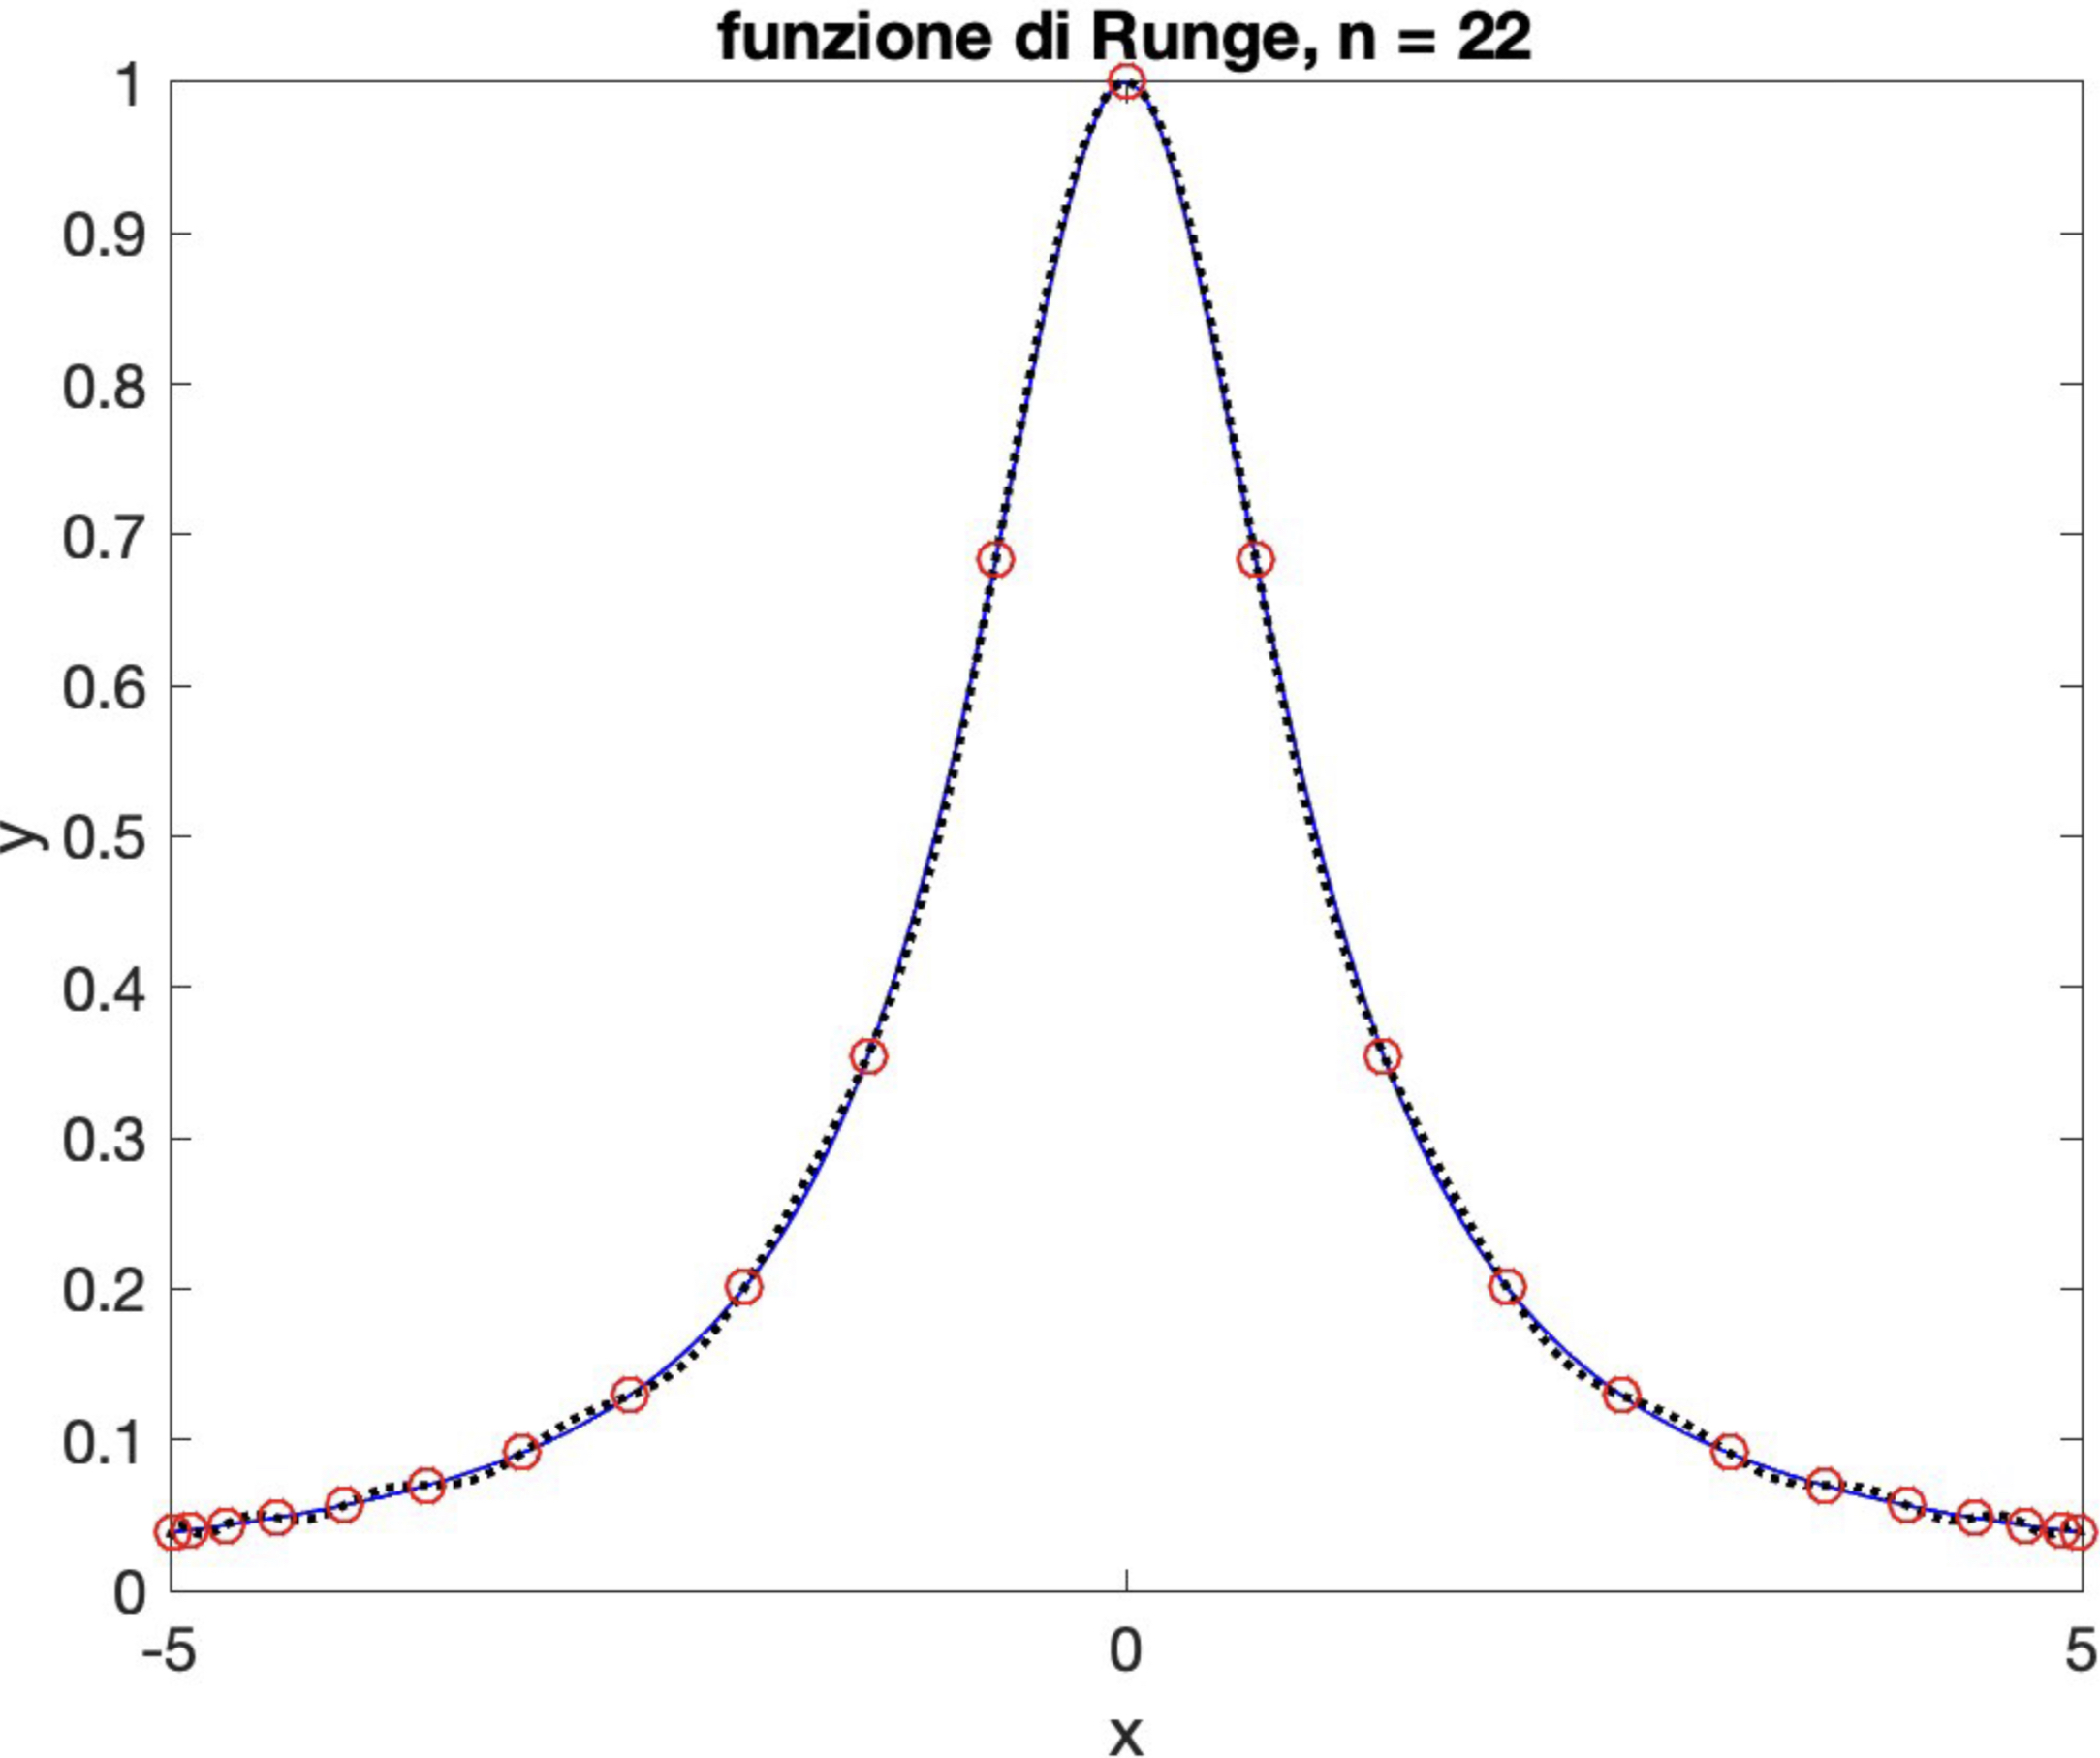
\includegraphics[width=0.5\textwidth]{immagini/fRungeAscChebN=22.jpg}
    \caption{Esempio di crescita di $\Lambda_n$ al crescere di $n$.}\label{fig:fRungeAscChebN=22}
\end{figure}

\subsection{Interpolazione mediante funzioni spline} \footnote{Slide 10-15 PDF 22, Slide 2-3 PDF 23, PG 94 - 100.}
Dalle Figure \ref{fig:fRungeAscChebN=2}-\ref{fig:fRungeAscChebN=22} è possibile ottenere che l'approssimazione migliora all'aumentare del numero di ascisse. Inoltre, è necessario notare che 40 è il numero limite di ascisse per il quale l'approssimazione non migliora, anche se queste sono aumentate. Questo è dovuto al fatto che il numero di condizionamento, pur non essendo particolarmente grande, è influenzato dagli errori di round-off.

In analisi matematica i problemi sono concepiti in aritmetica infinita (ovvero esatta),  ma gli algoritmi sono in aritmetica finita (il problema rappresentato è perturbato, in quanto non è quello reale). Al crescere della grado del polinomio interpolante, le ascisse di Chebyshev evidenziano i limiti dell'utilizzo dell'aritmetica finita, dove il problema è quello di valutare un polinomio di grado elevato in aritmetica finita.

La necessità, quindi, è quella di definire un algoritmo poco sensibile a perturbazioni. Se il numero di ascisse è fatto tendere all'infinito allora l'errore tenderà a 0, ma se è considerato l'errore di round-off accade che gli errori, dovuti all'approssimazione, sono più piccoli degli errori di round-off e sotto questo livello non è possibile scendere. Lo scopo è quello di fornire una soluzione a questo problema tramite ciò che sarà introdotto.

Il punto di partenza per la definizione dell'algoritmo prima citato è il Teorema di Jackson (Teorema \ref{th:Jackson}), il quale lega l'errore di approssimazione al condizionamento del problema tramite la maggiorazione (\ref{eq:maggErrMiglAprrox}). Il problema con la maggiorazione (\ref{eq:maggErrMiglAprrox}) è il seguente: aumentando il grado $n$ del polinomio, il modulo di continuità $\omega$ è reso sempre più piccolo e non è assicurato che non possa essere migliore (così facendo è possibile che venga modificata la decrescenza del modulo di continuità). Tuttavia, se $n$ è piccolo e l'intervallo $[a,b]$ è fissato, $\omega$ non potrà tendere a 0.

In alternativa all'approccio classico è possibile definire quanto segue.

\begin{definition}[Partizione di insieme]
    Dato $[a,b]$ dominio di $f$, una partizione $\Delta$ sull'intervallo $[a,b]$ è definita come
    \begin{equation}\label{eq:defPartizione}
            \Delta = \{\boldsymbol{a}=x_0<x_1<\hdots<x_n=\boldsymbol{b}\},
    \end{equation}
    la quale contiene $n+1$ punti (ovvero ascisse).
\end{definition}

\begin{definition}[Condizione di uniformità della partizione]
    La condizione di uniformità della partizione $\Delta$ (definita come (\ref{eq:defPartizione})) è definita come
    \begin{equation}\label{eq:condUnifPart}
        \boldsymbol h\overset{\footnotemark}{\boldsymbol =}\underset{\boldsymbol{i=1,\hdots,n}}{\boldsymbol\max}\boldsymbol{(x_i-x_{i-1}).}
    \end{equation}
\end{definition}
\footnotetext{Massima ampiezza tra i sottointervalli e la partizione. Ciò che è assunto è: aumentanto il numero dei punti $h\rightarrow 0$, quindi non rimangano zone dell'intervallo $[a,b]$ che, se il numero delle ascisse tende all'infinito, sono senza punti. Se sono aggiunti punti questi sono aggiunti per tutti. Una partizione uniforme garantisce queste proprietà, ovvero (\ref{eq:condUnifPart}).}

È assunto che $h\rightarrow 0,\, n\rightarrow\infty$. Inoltre, è assunto che su ciascun sottointervallo $[x_{i-1}, x_i],\, i=1,\hdots, n$, di $\Delta$ è utilizzato un polinomio di \textbf{grado $\boldsymbol m$ fissato}, interpolante $f(x)$ agli estremi del sottointervallo. Quindi, la nuova funzione interpolante è polinomiale a tratti (ovvero, in ogni sottointervallo è presente un polinomio).
Così facendo, (\ref{eq:maggErrMiglAprrox}) diviene
\begin{equation*}
    \underset{\footnotemark}{||e||}\leq\underbrace{\alpha (1+\Lambda_m)}_{\text{non varia}}\underbrace{\omega\left(f;\frac{h}{m}\right)}_{\text{tende a 0}},
\end{equation*}
dove:
\footnotetext{Se $f$ e $p$ hanno grado $m$, significa che la costante di Lebesque si trasforma in $\Lambda_m$, la quale è fissata, non cambia, ed al posto di $\frac{b-a}{m}$ è inserita la massima ampiezza dell'intervallo.}
\begin{itemize}
    \item $\boldsymbol{m}$ è fissato,
    \item $h\rightarrow 0$, se $\boldsymbol{n}\rightarrow\infty$,
\end{itemize}
con $m$ ed $n$ svincolati.

\footnote{La strategia è dividere il problema in tanti sottoproblemi, ciascuno di essi utilizza un polinomio interpolante di grado fissato $m$ solo agli estremi dell'intervallo.} Date le due precedenti definizioni, il problema del condizionamento diviene meno importante perché $m$ è fissato mentre, se $f\in C^{(0)}$ (vedi (\ref{eq:modCont})), vale il Teorema \ref{th:modContInf}.

Con una lente più formale è possibile definire quanto segue:
\begin{definition}[Spline di $m$ su $\Delta$]\label{def:spline}
    \footnote{Definizione 1 Slide 11 PDF 22, Definizione 4.3 PG 94.}
    $s_m(x)$ è una funzione definita come spline di grado $m$ sulla partizione $\Delta$, la quale è definita come (\ref{eq:defPartizione}), se:
    \begin{enumerate}
        \item $s_m(x)\in C^{(m-1)}[a,b]$; \footnotemark
        \item $s_m|_{[x_{i-1},x_i]}(x)\in\Pi_m,\,\forall i=1,\hdots,n.$
    \end{enumerate}
\end{definition}
\footnotetext{$s_m$ deve essere derivabile $m-1$ volte e le $m-1$ derivate devono essere continue. Se $s_m$ è un polinomio allora soddisferà la condizione perché un polinomio è $C^\infty$ (le derivate successive sono nulle).}

1. e 2. sono condizioni diverse: 1. definisce cos'è una spline di grado $m$ e 2. afferma che la spline coincide con il grado assegnato in ciascun sottointervallo. Una spline interpolante soddisfa le condizioni di interpolazione solite (ovvero $n+1$). È necessario imporre sulla 2. la condizione (\ref{eq:condInterpSpline2}).

\begin{remark}\label{rem:n+mCondIndip}
    \footnote{Slide 12 PDF 22, Teorema 4.11 PG 95.} Denotando con $\boldsymbol{S_m(\Delta)}$ l'insieme delle spline di grado $m$ sulla partizione $\Delta$, contenente $n+1$ ascisse, questo è uno \textbf{spazio vettoriale} di dimensione $\boldsymbol{m+n}$.
\end{remark}

La dimensione di uno spazio vettoriale è importante per individuare una spline univocamente. Un risultato importante dell'Osservazione \ref{rem:n+mCondIndip} è il seguente: è possibile individuare in modo univoco una spline di grado $m$ sulla partizione $\Delta$, con $m+n$ condizioni distinte, quindi indipendenti. Inoltre, la dimensione di uno spazio vettoriale è utilizzata per determinare quante condizioni sono necessarie per individuare un oggetto.

\begin{remark}
    \footnote{Slide 12 PDF 22.} $\Pi_m\subset S_m(\Delta).$
\end{remark}

Dalla precedente osservazione è possibile dedurre che lo spazio vettoriale dei polinomi di grado al più $m$ è contenuto nell'insime delle spline di grado $m$. Inoltre, è necessario ricordare che il polinomio di grado $m$ è una funzione $C^\infty$ e, rispetto a ciascun sottointervallo, coincide con se stesso.

\begin{definition}\label{def:interpFInDelta}
    \footnote{Definizione 2 Slide 12 PDF 22, Definizione 4.4 PG 95. Ciò che è tra parentesi è un aggiunta maggiore chiarezza. Date le condizioni 1. e 2. della Definizione \ref{def:spline} è possibile dare la seguente definizione.}
    Una spline $s_m(x)$ sulla partizione $\Delta$ interpola una funzione $f(x)$ (nei nodi della partizione) se (valgono le seguenti condizioni di interpolazione): 
    \begin{equation}\label{eq:condInterpSpline}
        \boldsymbol{s_m(x_i)=f(x_i)\equiv f_i,\quad i=0,\hdots,n.}
    \end{equation}
\end{definition}

La definizione aggiunge alle due condizione necessarie affinché $s_m(x)$ sia definita spline, le condizioni necessarie affinché $s_m(x)$ interpoli $f(x)$.

\begin{remark}
    \footnote{Slide 13 PDF 22, PG 95.} Le sole condizioni di interpolazione ($n+1$) permettono di individuare univocamente le spline di grado 1, anche dette spline lineari. In questo caso una spline lineare è la spezzata che congiunge i punti di interpolazione $(x_i,f_i),$ per $i=0,\hdots, n$. La spline lineare interpolante è data da 
    \begin{equation}\label{eq:splineLineare}
        \boldsymbol{s_1|_{[x_{i-1}, x_i]}(x)=\frac{(x-x_{i-1})f_i+(x_i-x)f_{i-1}}{x_i-x_{i-1}},\quad i=1,\hdots,n.}
    \end{equation}
\end{remark}

\begin{figure}
    \centering
    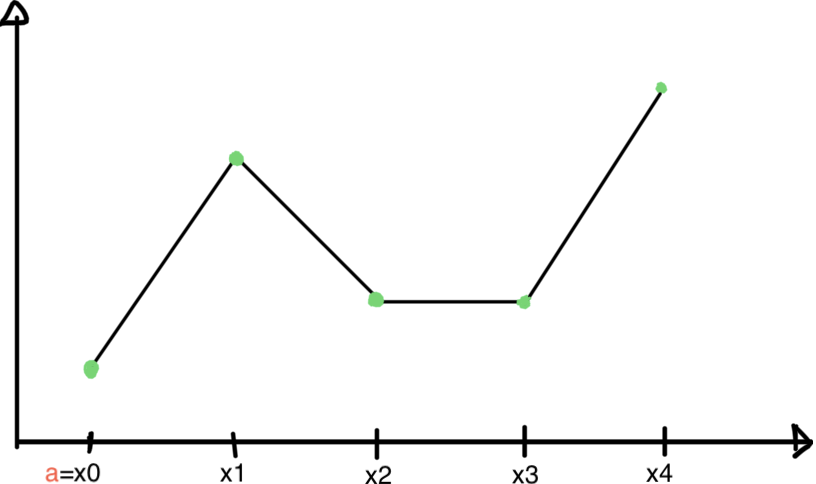
\includegraphics[width=0.5\textwidth]{immagini/s_mN=4.png}
    \caption{Esempio di spline con $n=4$.}\label{fig:s_mN=4}
\end{figure}

Quindi $s_1(x)$ è il segmento che congiunge i punti in coordinate $(x_{i-1},f_{i-1})$ e $(x_i,f_i)$. Questo sarà utile quando saranno calcolate spline diverse dalle lineari.

La definizione di spline di grado $m$ (Definizione \ref{def:spline}) prescinde dal fatto che la spline sia interpolante la funzione. All'interno dello spazio vettoriale l'obbiettivo è quello di individuare una spline interpolante, possibilmente unica.
Quando il grado della spline aumenta allora esistono diverse spline di grado superiore, per le quali ciascuna sarà una spline di grado $m$ interpolante. Queste spline differendo per poco, dato che le condizioni mancanti saranno imposte e ciascuna scelta riguardo le condizioni imposte genera spline diverse.

La condizione 1. della Definizione \ref{def:spline} implica che la spline $s_m$ debba essere una funzione di classe $C^{(m-1)}[a,b]$. Questo requisito richiede di imporre delle condizioni sui punti interni della partizione $x_1,\hdots,x_{n-1}$, ovvero i punti di contiguità tra i sottointervalli $[x_{i-1},x_i]$ e $[x_i,x_{i+1}],$ per $ i=1,\hdots,n-1$. Ovvero, le condizioni da imporre sono le seguenti:
\begin{equation}\label{eq:condInterpSpline2}
    \begin{matrix}
        s_m^{(\boldsymbol{j})}|_{[x_{i-1},\boldsymbol{x_i}]}(\boldsymbol{x_i})= s_m^{(\boldsymbol{j})}|_{[\boldsymbol{x_i},x_{i+1}]}(\boldsymbol{x_i}),\\
        j=0,\hdots,m-1,\; i=1,,\hdots,n-1.
    \end{matrix}
\end{equation}

\noindent\footnotemark In altri termini, i due polinomi devono raccordarsi fino alla derivata $m-1$ nel punto $x_i$. Quando $j=0$ è richiesta solo la continuità, se è ricercata una spline interpolante in quei punti "viene gratis". Entrambi i polinomi devono assumere il valore della funzione che sta essendo interpolata. Il problema sono le derivate successive.
\footnotetext{Significa che sono presenti due sottointervalli contigui: a sinistra del primo sottointervallo la spline coincide con un polinomio, nel secondo sottointervallo con un altro polinomio di grado $n$. La $j$ rappresenta la derivata $j$-esima di $s_m$ e $x_i$ il punto continguo degli insiemi.}

Vale il seguente risultato.

\begin{theorem}\label{th:gradoDervSpline}
    \footnote{Slide 14 PDF 22, Teorema 4.10 PG 95} Se $s_m$ è una spline di grado $m\geq 2$ sulla partizione $\Delta$, allora $s'_m(x)$ è una spline di grado $m-1$ sulla stessa partizione.
\end{theorem}
\begin{proof}
    Se $s_m(x)$ è una spline di grado $m\geq 2$ sulla partizione $\Delta$, allora:
    \begin{enumerate}
        \item $s_m(x)\in C^{(m-1)}[a,b]\overset{\footnotemark}{\Rightarrow} s'_m(x)\in C^{(m-2)}[a,b];$
        \footnotetext{Data una funzione di una qualsiasi classe $m$ allora la sua derivata è di $m-1$. È eliminata un'equazione ma le successive derivate rimangono.}
        \item $s_m|_{[x_{i-1},x_i]}(x)\in\Pi_m,\,\forall i=1,\hdots,n\Rightarrow s'_m|_{[x_{i-1},x_i]}(x)\in\Pi_{m-1},\;\forall i=1,\hdots,n.$
    \end{enumerate}
    Pertanto, $s'_m\in S_{m-1}(\Delta).$
\end{proof}
Dato che $m\geq 2\,(>0)$, per il Teorema, quindi la funzione è continua (questo vale anche per le funzioni lineari). ($C^{-1}$ significa che la funzione è costante.)

\subsection{Spline cubiche}
\begin{remark}
    \footnote{Slide 15 PDF 22.}
    Nella pratica computazionale assumono particolare importanza le \textbf{spline cubiche ($\boldsymbol{m=3}$)}. Se è ricercata la spline cubica interpolante sono necessarie due ulteriori condizioni, ognuna delle quali darà origine ad una spline cubica interpolante generalmente diversa, oltre alle condizioni definite in (\ref{eq:condInterpSpline}). Una funzione di grado 3 sarà interpolata da un polinomio di grado 3 e può accadere che più spline coincidano.
\end{remark}

I motivi per i quali è scelta la spline cubica sono le condizioni solitamente asimmetriche rispetto agli estremi dell'intervallo. La derivata prima di una spline quadratica è continua, ha un profilo smooth e per questo sono scelte per l'approssimazione di funzioni. Sono utilizzate le spline cubiciche e non quadratiche dato che l'unica condizione è la non simmetria.

Per individuare univocamente una spline cubica definita sulla partizione $\Delta$, occorrono $n+3$ ($m=3$) condizioni indipendenti tra loro. Se è ricercata una spline interpolante una data funzione $f(x)$, le condizioni di interpolazione (\ref{eq:condInterpSpline}) forniscono $n+1$ condizioni. Pertanto, rimangono da fissare \textbf{2 condizioni addizionali} per determinare univocamente una spline cubica, dove ciascuna coppia di condizioni addizionali darà origine ad una spline interpolante, le quali sono \textbf{generalmente diverse tra loro.} Le condizioni di interpolazione sono importanti ed esiste un certo numero di modi per imporle, ciascuno di questi modi genererà una spline interpolante, generalmente le spline generate sono diverse.

Sono esaminante \textbf{4 possibili implementazioni} delle condizioni aggiuntive e neccessarie da imporre per determinare una spline cubica interpolante.
\subsubsection{Spline cubica naturale}
\footnote{Slide 4 PDF 23, PG 96.} 
Questa spline è determinata dalle due seguenti condizioni:
\begin{equation}\label{eq:condSplineCubNat}
    \boxed{s''_3(a)=0,\quad s''_3(b)=0.}
\end{equation}

La spline cubica naturale è quella che minimizza la curvatura totale della curva (non sarà trattato). Questa spline è scelta perché porta all'algoritmo di misurazione più efficiente tra tutti (non sarà trattato).

\subsubsection{Spline cubica completa}\footnote{Nota precedente.}
Questa spline è determinata dalle due seguenti condizioni:
\begin{equation}\label{eq:condSplineCubComp}
    \boxed{s'_3(a)=f'(a),\quad s'_3(b)=f'(b)}
\end{equation}

Negli estremi della partizione $\Delta$ è imposta una condizione di interpolazione di Hermite.
Dal punto di vista computazionale è implementata con variazioni della spline cubica naturale.

\subsubsection{Spline cubica interpolante periodica} \footnote{Nota precedente. Questa non è applicata ad una funzione interpolanda ma a funzioni periodiche.}
Questo tipo di spline è utilizzata supponendo che la funzione $f(x)$ sia una funzione periodica sull'intervallo $[a,b]$. Infatti vale la segeunte osservazione:

\begin{remark}
    Quanto scritto significa che $b-a$, che è l'ampiezza dell'intervallo, deve essere un multiplo intero del periodo $T$ della funzione [\footnote{È possibile un'efficienza maggiore esprimendo $b$ come $b=T\cdot a$.}].
\end{remark}

\begin{example}
    Se $f(x)=\sin(x)\Rightarrow b$ deve essere un multiplo di $2\pi$, altrimenti la funzione non è periodica (ad esempio con $[0,\pi]$).
\end{example}

Dalle condizioni di interpolazioni e per la periodicità di $f(x)$, è noto quanto segue:
\begin{equation*}
    s_3(a)=f(a)=f(b)=s_3(b).
\end{equation*}

Se $\boldsymbol{f(x)\in C^{(2)}[a,b]}$, ovvero $f$ è più che continua, \textbf{come funzione periodica}, allora:

\begin{equation}\label{eq:condPeriod}
    f'(a)=f'(b),\quad f''(a)=f''(b).
\end{equation}

Dato che è richiesto che la spline cubica $s_3\in C^{(2)}[a,b]$, per la definizione di spline (Definizione \ref{def:spline}), è imposto che lo sia anche come funzione periodica. Analogamente a (\ref{eq:condPeriod}), sono imposte le seguenti condizioni aggiuntive:

\begin{equation}\label{eq:condSplineCubPer}
    \boxed{s'_3(a)=s'_3(b),\quad s''_3(a)=s''_3(b).}
\end{equation}

\begin{remark}
    Questo tipo di spline è applicato esclusivamente al caso di funzioni periodiche sull'intervallo $[a,b]$.
\end{remark}

\paragraph{Intermezzo:}È possibile costruire spline cubiche interpolanti una funzione periodica  del tipo natuale, periodica e completa ottenendo risultati generalmente diversi fra loro.

\subsubsection{Spline cubica interpolante not-a-knot}
\begin{remark}\footnote{Slide 5 PDF 23, PG 97}
    Questa spline è implementata nella \textit{function \textbf{spline}} di Matlab.
\end{remark}

\textbf{Questa spline non necessita di ulteriori informazioni oltre a quelle di interpolazione}, le condizioni aggiuntive sono  imposte in modo implicito. 

È noto che nei primi due sottointervalli siano presenti due polinomi di grado 3 (e così anche negli ultimi due). Ciò che è richiesto è che i due polinomi ed i primi due sottoinsiemi, tramite l'unione ($[x_0,x_1]\cup[x_1,x_2]=[x_0,x_1]$), coincidano. In questo modo è imposta una condizione in meno in modo esplicito. 

La spline not-a-knot fa in modo che il nodo 1 ($x_1$) non sia il nodo che definisce una spline in senso classico. Questo è dovuto al fatto che è presente un unico polinomio nel primo e secondo sottoinsieme, in genere sono distinti. La stessa cosa avviene anche negli ultimi due sottointervalli.

Le condizioni aggiuntive sono imposte in modo implicito come segue:
\begin{enumerate}
    \item lo \textbf{stesso polinomio cubico definisce} la spline $\boldsymbol{s_3}$ \textbf{sui primi 2 sottointervalli} $\boldsymbol{[x_0,x_1]}$ e $\boldsymbol{[x_1,x_2]}$;
    \item \footnotemark \textbf{simmetricamente}, \textbf{lo stesso polinomio cubico} definisce la spline $s_3$ sugli ultimi due sottointervalli $[x_{n-2},x_{n-1}]$ e $[x_{n-1},x_n]$.
    \footnotetext{La condizione di simmetria è importante perché, data la funzione $f(x)$, è definita $g(x)$ come $f$ rovesciando la direzione di $x$. $g(a)=f(b)$ se $f(x)$ e $g(x)$ hanno lo stesso verso. Le due funzioni hanno lo stesso grafico ed è importante che abbiano la stessa approssimazione. Sotto le stesse condizioni è ottenuto lo stesso risultato.}
\end{enumerate}

Imporre questa condizione per la 1. significa quanto segue (similmente per 2.):
\begin{equation*}
    p_1(x)=s_3|_{[x_0,x_1]}(x),\quad p_2(x)=s_3|_{[x_1,x_2]}(x),
\end{equation*}
dove è ricercato $p_1(x)=p_2(x)\in\overset{\footnotemark}{\Pi_3}$. In $x_1$, tramite le condizioni di interpolazione, è ottenuto $p_1(x_1)=p_2(x_1)$. Il raccordo deve valere anche per le derivate prima e seconda, ovvero:
\begin{equation*}
    p'_1(x_1)=p'_2(x_1)\quad\land\quad p''_1(x_1)=p''_2(x_1).
\end{equation*}
\footnotetext{Un polinomio di grado 3 ha 4 coefficienti, 4 gradi libertà e $\Pi_3$ è uno spazio vettoriale di dimensione 4.}

Se è imposto che $\overset{\footnotemark}{p'''_1(x_1)}\overset{\footnotemark}{=}\overset{\footnotemark}{p'''_2(x_1)}$ allora $p_1(x)=s_3(x)=p_2(x),\, x\in [x_0,x_2]$. Quindi, definita la spline $s_3(x)$ e le sue derivate come 
\begin{equation*}
    \begin{matrix}
        s_3|_{[x_0,x_2]}(x)\in\Pi_3,\\
        s'_3|_{[x_0,x_2]}(x)\in\Pi_2,\\
        s''_3|_{[x_0,x_2]}(x)\in\Pi_1,\\
        \underset{\footnotemark}{s'''_3|_{[x_0,x_2]}(x)}\in\Pi_0,
    \end{matrix}
\end{equation*}
è possibile imporre condizione sui primi due sottintervalli della partizione $\Delta$, la quale è
\begin{equation*}
    \boxed{\frac{s''_3(\boldsymbol{x_1})-s''_3(x_0)}{x_1-x_0}=\frac{s''_3(x_2)-s''_3(\boldsymbol{x_1})}{x_2-x_1}.}
\end{equation*}

\addtocounter{footnote}{-3}
\footnotetext{Restrizione sul primo sottointervallo.}

\stepcounter{footnote}
\footnotetext{È presente un raccordo $C^{(2)}$ nel punto di continuità ed è noto il raccordo della derivata terza. Inoltre, la funzione ha derivate che coincidono in più punti, quando due polinomi sono lo stesso, per $x\in [x_0,x_1]\cup[x_1,x_2]=[x_0,x_2]$. Le precedenti sono 4 condizioni distinte con 4 gradi di libertà.}

\stepcounter{footnote}
\footnotetext{Restrizione sul secondo sottointervallo.}

\stepcounter{footnote}
\footnotetext{Questo polinomio di grado 0 è una costante, il coeffciente lineare della retta derivata seconda, ed è la stessa a sinistra ed a destra di $x_1$. Questo significa che il rapporto incrementale della derivata seconda su $x_0,\, x_1$ e $x_2$  deve essere lo stesso.}

Simmetricamente, sugli ultimi due sottointervalli, sarà imposto:
\begin{equation*}
    \boxed{\frac{s''_3(x_n)-s''_3(\boldsymbol{x_{n-1}})}{x_n-x_{n-1}}=\frac{s''_3(\boldsymbol{x_{n-1}})-s''_3(x_{n-2})}{x_2-x_1}.}
\end{equation*}

$\boldsymbol{x_1}$ e $\boldsymbol{x_{n-1}}$ precedenti non sono considerati nodi della partizione in quanto sono imposte le condizioni di interpolazione e le condizioni di default.

Ciò che è stato appena definito nei riquadri è una conveniente espressione, in virtù del Teorema \ref{th:gradoDervSpline}, delle condizioni aggiuntive della spline cubica not-a-knot, ovvero:
\begin{equation}\label{eq:condSplineCubNotAKnot}
    s'''_3|_{[x_0,x_1]}(x_1)=s'''_3|_{[x_1,x_2]}(x_1),\quad s'''_3|_{[x_{n-2},x_{n-1}]}(x_{n-1})=s'''_3|_{[x_{n-1},x_n]}(x_{n-1}).
\end{equation}

La rappresentazione delle condizioni (\ref{eq:condSplineCubNotAKnot}) tramite le derivate seconde è utile al fine di definire l'unicità della spline interpolante. Dal punto di vista computazionale è importante che le condizioni siano imposte sulla derivata seconda.

\begin{remark}
    \footnote{Slide 2 PDF 24, Osservazione 4.5 PG 97.} L'ampiezza dell'intervallo $i$-esimo della partizione $\Delta$, definita come (\ref{eq:defPartizione}), è definita come
    \begin{equation}\label{eq:defAmpiezzaInt}
        \boldsymbol{h_i=x_i-x_{i-1},\quad i=1,\hdots,n},
    \end{equation}
    dove la massima ampiezza definita come 
    \begin{equation*}
        \boldsymbol{h=\underset{i=1,\hdots,n}{max}h_i},
    \end{equation*}
    allora è possibile dimostrare, se $f\in C^{(4)}[a,b]$, che per tutte le spline cubiche esaminate vale
    \begin{equation*}
        \left|\left|f^{(i)}-s^{(i)}_3\right|\right|=O\left(h^{4-i}\right),\quad i=0,1,2.
    \end{equation*}
\end{remark}

Quanto osservato significa che le spline cubiche consentono di approssimare efficientemente funzioni regolari, senza preoccuparsi troppo della scelta della partizione (ad esempio quella uniforme è sufficiente).

Approssimare la funzione significa approssimare uniformemente anche la derivata prima e seconda. Questo risultato è esatto per tutte le spline cubiche tranne per la naturale, dove, se forzata, la derivata seconda negli estremi è 0. Questo non è sempre vero in quanto è possibile introdurre errori sistematici. È possibile affermare che l'errore diminuisce rapidamente quando è ottenuto dagli estremi dell'intervallo.

\subsection{Calcolo (pratico) di una spline cubica}\label{ssec:calcSplineCub}\footnote{Slide 2-13 PDF 24, PG 97-101.}
Per trattare questa Sezione è utile la Sezione \ref{ssec:risSistTridiag}.

Il problema da affrontare è quello del calcolo della spline cubica $s_3(x)$ interpolante $f(x)$ sulla partizione, definita come in (\ref{eq:defPartizione}), $\Delta=\{a=x_0<x_1<\hdots<x_n=b\}$.

Per determinare un algoritmo efficiente per il calcolo di una spline cubica, oltre a (\ref{eq:defAmpiezzaInt}), sarà usata la notazione seguente:
\begin{equation}\label{eq:s''3(xi)}
    \boldsymbol{m_i=s''_3(x_i),\quad i=0,\hdots,n.}
\end{equation}

In particolare saranno esaminati gli algoritmi per il calcolo delle spline cubiche naturali e not-a-knot. Sarà altresì trattato come, utilizzando questi argomenti, con piccoli cambiamenti, possono essere ottenute le spline naturali e complete. È necessario individuare quali siano le condizioni, in termini di $m_i$ definiti tramite (\ref{eq:s''3(xi)}), che caratterizzano l'un l'altra.

Il calcolo della spline cubica naturale è semplice ed, inoltre, è stato trattato come le condizioni imposte riguardino l'annullamento della derivata seconda, negli estremi $a$ e $b$. L'annullamento della derivata seconda e la notazione (\ref{eq:s''3(xi)}) implicano che, per una \textbf{spline cubica naturale}, le condizioni diventino
\begin{equation}\label{eq:condSplineNat}
    \boldsymbol{m_0=0=m_n}.
\end{equation}

Imponendo (\ref{eq:defAmpiezzaInt}), \textbf{le condizioni aggiuntive della spline not-a-knot}, ovvero degli estremi sinistro e destro (\ref{eq:condSplineCubNotAKnot}), diventano
\begin{equation*}
    \frac{m_1-m_0}{h_1}=\frac{m_2-m_1}{h_2},\quad \frac{m_{n-1}-m_{n-2}}{h_{n-1}}=\frac{m_n-m_{n-1}}{h_n}
\end{equation*}
ovvero $h_2(m_1-m_0)=h_1(m_2-m_1),\, h_{n}(m_{n-1}-m_{n-2})=h_{n-1}(m_{n}-m_{n-1})$, dalle quali sono ottenute le condizioni
\begin{equation}\label{eq:condSplineCubNotAKnot2}
    \boldsymbol{h_2m_0-(h_1+h_2)m_1+h_1m_2=0}\quad\boldsymbol{h_{n-1}m_n-(h_{n-1}+h_n)m_{n-1}+h_nm_{n-2}=0}.
\end{equation}

\textbf{(\ref{eq:condSplineCubNotAKnot2}) sono le condizioni aggiuntive per le spline not-a-knot}.

Riguardo le altre condizioni $\{m_i\}$, è possibile osservare che, se $s_3(x)$ è una spline cubica sulla partizione $\Delta$, allora $s'_3(x)$ è una spline di grado 2 sulla stessa partizione, e $s''_3(x)$ è una spline lineare su $\Delta$. Pertanto, essendo $s''(x)$ una spline lineare, da (\ref{eq:splineLineare}) e (\ref{eq:s''3(xi)}), è ottenuto che
\begin{equation*}
    s''_3(x)\underset{\footnotemark}{=}\frac{(x-x_{i-1})m_i+(x_i-x)m_{i-1}}{\equalto{h_i}{x_i-x_{i-1}}},\quad\boldsymbol{x\in[x_{i-1}, x_i]},\; i=1,\hdots,n.
\end{equation*}\footnotetext{Le $m_i$ non sono note. Sono noti i valori della derivata seconda della spline che assume nelle asisse di interpolazione. Quindi la derivata seconda della spline è la spline lineare che interpola gli $m_i$.}

Integrando membro a membro la precedente equazione è ottenuto
\begin{equation}\label{eq:s'_3(x)}
    s'_3(x)=\frac{(x-x_{i-1})^2m_i-(x_i-x)^2m_{i-1}}{2h_i}+\underset{\footnotemark}{q_i},\quad x\in [x_{i-1}, x_i],\; i=1,\hdots,n.
\end{equation}\footnotetext{Costante d'integrazione.}

\noindent\footnote{Non conoscendo le $m_i$ non è possibile calcolare la derivata seconda. Integrando membro a membro sarà ottenuta la derivata prima della spline e questa sarà la restrizine all'$i$-esimo sottointervallo $[x_{i-1},x_i]$.}
Integrando nuovamente è ottenuta un'ulteriore spline:

\begin{equation}\label{eq:s3Ign}
    s_3(x)=\frac{(x-x_{i-1})^3\boldsymbol{m_i}+(x_i-x)^3\boldsymbol{m_{i-1}}}{6h_i}+\boldsymbol{q_i}(x-x_{i-1})+\underset{\footnotemark}{\boldsymbol{r_i}},\quad x\in[x_{i-1},x_i],\; i=1,\hdots,n.
\end{equation}\footnotetext{Nuova costante di integrazione.}

\noindent\footnote{Fossero noti gli $m_i$ e fosse possibile determinare le costanti di integrazione $r_i$ e $q_i$, allora sarebbe possibile calcolare il polinomio di grado 3, il quale costituisce la restrizione della spline nell'intervallo d'interesse. Ciò che sarà richiesto nell'elaborato, quando sarà necessario calcolare la spline nei punti assegnati, sarà calcolare la spline nei punti interpolanti. Adesso saranno eliminate le costanti $q_i$ e $r_i$ imponendo condizione di interpolazione agli estremi di ciascun sottointervallo.}
Imponendo le condizioni di interpolazione a ciascun intervallo, è ottenuto quanto segue:
\begin{itemize}
    \item $s_3(x_1)=\frac{h_i^2}{6}m_{i-1}+r_i=f(x_{i-1})$, dalla quale è ottenuta \begin{equation}\label{eq:ri}
        \underset{\footnotemark}{\boldsymbol{r_i}}\boldsymbol{=f(x_{i-1})-\frac{h_i^2}{6}m_{i-1}},
    \end{equation}
    dove $f(x_{i-1})$ ed $h_i^2$ sono valori noti.
    \item $s_3(x_i)=\frac{h_i^2}{6}m_i+q_ih_i+r_i\overset{\footnotemark}{=}f(x_i)$. Pertanto,
    \begin{equation*}
        \begin{matrix}
             h_iq_i &=& f(x_i)-r_i-\frac{h_i^2}{6}m_i &\overset{\footnotemark}{=}& f(x_i)-f(x_{i-1})+\frac{h_i^2}{6}(m_{i-1}-m_i) &\Rightarrow&\\
            &\Rightarrow& q_i &=& \frac{f(x_i)-f(x_{i-1})}{\underbrace{x_i-x_{i-1}}_{h_i}}+\frac{h_i}{6}(m_{i-1}-m_i).&&
        \end{matrix}
    \end{equation*}
    Da cui,
    \begin{equation}\label{eq:qi}
        \boldsymbol{q_i=f[x_{i-1},x_i]+\frac{h_i}{6}(m_{i-1}-m_i).}
    \end{equation}
\end{itemize}
\addtocounter{footnote}{-2}
\footnotetext{Non calcolabile perché le $m_i$ non sono note.}

\stepcounter{footnote}
\footnotetext{Con questa uguaglianza sono ricavate le $g_i$ perché le $r_i$ sono state calcolate.}

\stepcounter{footnote}
\footnotetext{Sostituzione di $r_i$ con (\ref{eq:ri}).}

Ora è necessario calcolare gli $\{m_i\}$, per poter calcolare le costanti $q_i$ e $r_i$ di ciascun sottointervallo $[x_{i-1},x_i]$ e quindi (\ref{eq:s3Ign}).

Imponendo che $s'_3(x)$ sia continua nei punti $x_i,\; i=1,\hdots,n$, ovvero imponendo che
\begin{equation*}
    s'_3|_{[x_{i-1}, x_i]}(x_i)=s'_3|_{[x_i, x_{i+1}]}(x_i),
\end{equation*}
è ottenuto, da (\ref{eq:s'_3(x)}):
\begin{equation*}
    \frac{h_i}{2}m_i+q_i=-\frac{h_{i+1}}{2}m_i+q_{i+1},\quad i=1,\hdots,n-1.
\end{equation*}

Quindi [\footnotemark]:
\begin{equation*}
    3h_im_i+h_i(m_{i-1}-m_i)+3h_{i+1}m_i-h_{i+1}(m_i-m_{i+1})=6\left(f[x_i,x_{i+1}]-f[x_{i-1},x_i]\right),\quad i=1,\hdots,n-1.
\end{equation*}
\footnotetext{Moltiplicando per 6 e portando a sinistra dell'uguale tutto ciò che dipende da $m$, è ottenuto quanto segue.}
Raggruppando gli $m_i$ con gli stessi indici a primo membro è ottenuto quanto segue:
\begin{equation*}
    h_im_{i-1}+2(h_i+h_{i+1})m_i+h_{i+1}m_{i+1}=6(f[x_i,x_{i+1}]-f[x_{i-1},x_i]),\quad i=1,\hdots,n-1.
\end{equation*}
Dividendo membro a membro per $h_i+h_{i+1}=x_{i+1}-x_{i-1},$ è ottenuto:
\begin{equation}\label{eq:eqCalcMi}
    \begin{matrix}
        \equaltoup{\boxed{\frac{h_i}{h_i+h_{i+1}}}}{\varphi_i}\,m_{i-1}+2m_i+\equaltoup{\boxed{\frac{h_{i+1}}{h_i+h_{i+1}}}}{\xi_i}\,m_{i+1}&=&6\,\frac{f[x_i,x_{i+1}]-f[x_{i-1},x_i]}{x_{i+1}-x_{i-1}}&\overset{\footnotemark}{=}&6\,f[x_{i-1},x_i,x_{i+1}],\\
        && && i=1,\hdots,n-1.
    \end{matrix}
\end{equation}\footnotetext{Per (\ref{eq:P5DiffDiv}).} 

\begin{remark}\label{re:varphi+xi=1}\footnote{Slide 9 PDF 24.}
    $\boldsymbol{\varphi_i,\, \xi_i>0,\, \varphi_i+\xi_i=1.}$
\end{remark}

Le equazioni (\ref{eq:eqCalcMi}) sono un sistema di $n-1$ equazioni nelle $n+1$ incognite $\{m_0,\hdots,m_n\}$.

\textbf{Nel caso} di \textbf{spline naturali}, tenendo di conto delle condizioni (\ref{eq:condSplineNat}), è \textbf{ottenuto il sistema tridiagonale} 
\begin{equation*}
    \begin{pmatrix}
        2 & \xi_1 & && \\
        \varphi_2 & 2 & \xi_2&&\\
        &\ddots & \ddots &\ddots&\\
        &&\ddots & \ddots &\xi_{n-2}\\
        &&&\varphi_{n-1} & 2
    \end{pmatrix}\begin{pmatrix}
        m_1\\
        m_2\\
        \vdots\\
        \vdots\\
        m_{n-1}
    \end{pmatrix}=6\begin{pmatrix}
        f[x_0,x_1,x_2]\\
        f[x_1,x_2,x_3]\\
        \vdots\\
        \vdots\\
        f[x_{n-2},x_{n-1},x_n]
    \end{pmatrix}.
\end{equation*}

Dall'Osservazione \ref{re:varphi+xi=1} è possibile notare che la matrice dei coefficienti è diagonale dominante sia per righe che per colonne e quindi la sua fattorizzazione $LU$ è definita\textbf{. Calcolati i valori} $\boldsymbol{\{m_i\}}$ \textbf{incogniti, la spline naturale è calcolata sostituendoli, assieme a (\ref{eq:ri})-(\ref{eq:qi}), in (\ref{eq:s3Ign}).}

Ragionamento analogo vale \textbf{per la spline cubica not-a-knot} ottenenuta imponendo le relative condizioni aggiuntive, per la quale \textbf{le condizioni (\ref{eq:condSplineCubNotAKnot2}) e (\ref{eq:eqCalcMi}) danno origine al sistema lineare}
\begin{equation}\label{eq:sisTridSpline}
    \begin{pmatrix}
        \xi_1 & -1 & \varphi_1 && \\
        \varphi_1 & 2 & \xi_1&&\\
        &\ddots & \ddots &\ddots&\\
        &&\varphi_{n-1}& 2 &\xi_{n-1}\\
        && \xi_{n-1} & -1 & \varphi_{n-1}
    \end{pmatrix}\begin{pmatrix}
        m_0\\
        m_1\\
        \vdots\\
        m_{n}
    \end{pmatrix}=6\begin{pmatrix}
        0\\
        f[x_0,x_1,x_2]\\
        \vdots\\
        f[x_{n-2},x_{n-1},x_n]\\
        0
    \end{pmatrix}.
\end{equation}

Sostituendo alla prima equazione la somma delle prime due, all'ultima la somma delle ultime due e moltiplicando a destra la matrice dei coefficienti per
\begin{equation*}
    \begin{pmatrix}
        1 & -1 & -1&&\\
        & 1 &&&\\
        &&\ddots&&\\
        &&&1&\\
        &&-1&-1&1
    \end{pmatrix} \begin{pmatrix}
        1 & 1 & 1&&\\
        & 1 &&&\\
        &&\ddots&&\\
        &&&1&\\
        &&1&1&1
    \end{pmatrix}\equiv I_{n+1},
\end{equation*}
il sistema lineare (\ref{eq:sisTridSpline}) è equivalente a
\begin{equation}
    \begin{matrix}
        \begin{pmatrix}
        1 & 0 & &&&& \\
        \varphi_1 & 2-\varphi_1 & \xi_1-\varphi_1&&&&\\
        &\varphi_2 & 2 &\xi_2&&&\\
        &&\ddots & \ddots &\ddots&&\\
        && & \varphi_{n-2} & 2&\xi_{n-2}&\\
        &&&&\varphi_{n-1}-\xi_{n-1} & 2-\xi_{n-1} &\xi_{n-1}\\
        &&&&& 0 & 1
    \end{pmatrix}\\
    \begin{pmatrix}
        m_0+m_1+m_2\\
        m_1\\
        \vdots\\
        m_{n-1}\\
        m_n+m_{n-1}+m_{n-2}
    \end{pmatrix}=6\begin{pmatrix}
        f[x_0,x_1,x_2]\\
        f[x_0,x_1,x_2]\\
        \vdots\\
        f[x_{n-2},x_{n-1},x_n]\\
        f[x_{n-2},x_{n-1},x_n]
    \end{pmatrix},
    \end{matrix}
\end{equation}
che risulta essere ancora tridiagonale e, avendo tutti i minori principali non nulli, fattorizzabile $LU$.

\subsection{Approssimazione polinomiale nel senso dei minimi quadrati}\label{ssec:approssimazione_polinomiale_minimi_quadrati}
\footnote{Slide 6-9 PDF 25, PG 101-104.} L'argomento trattato in questa Sezione è un diverso tipo di approssimazione. Spesso sono presenti troppi dati da approssimare affetti da errore, tipicamente senza bias, con una distribuzione gaussiana. Il concetto è che se il dato è affetto da errore interpolare non ha significato. È necessario trovare un'altra approssimazione ed a titolo di esempio sono presenti le Figure \ref{fig:4.10(1)}-\ref{fig:4.10(4)}.

Inoltre, è bene sottolineare che \textbf{è stato utilizzato} il termine "\textbf{Approssimazione}" \textbf{e non} "\textbf{Interpolazione}".

\begin{figure}
    \centering
    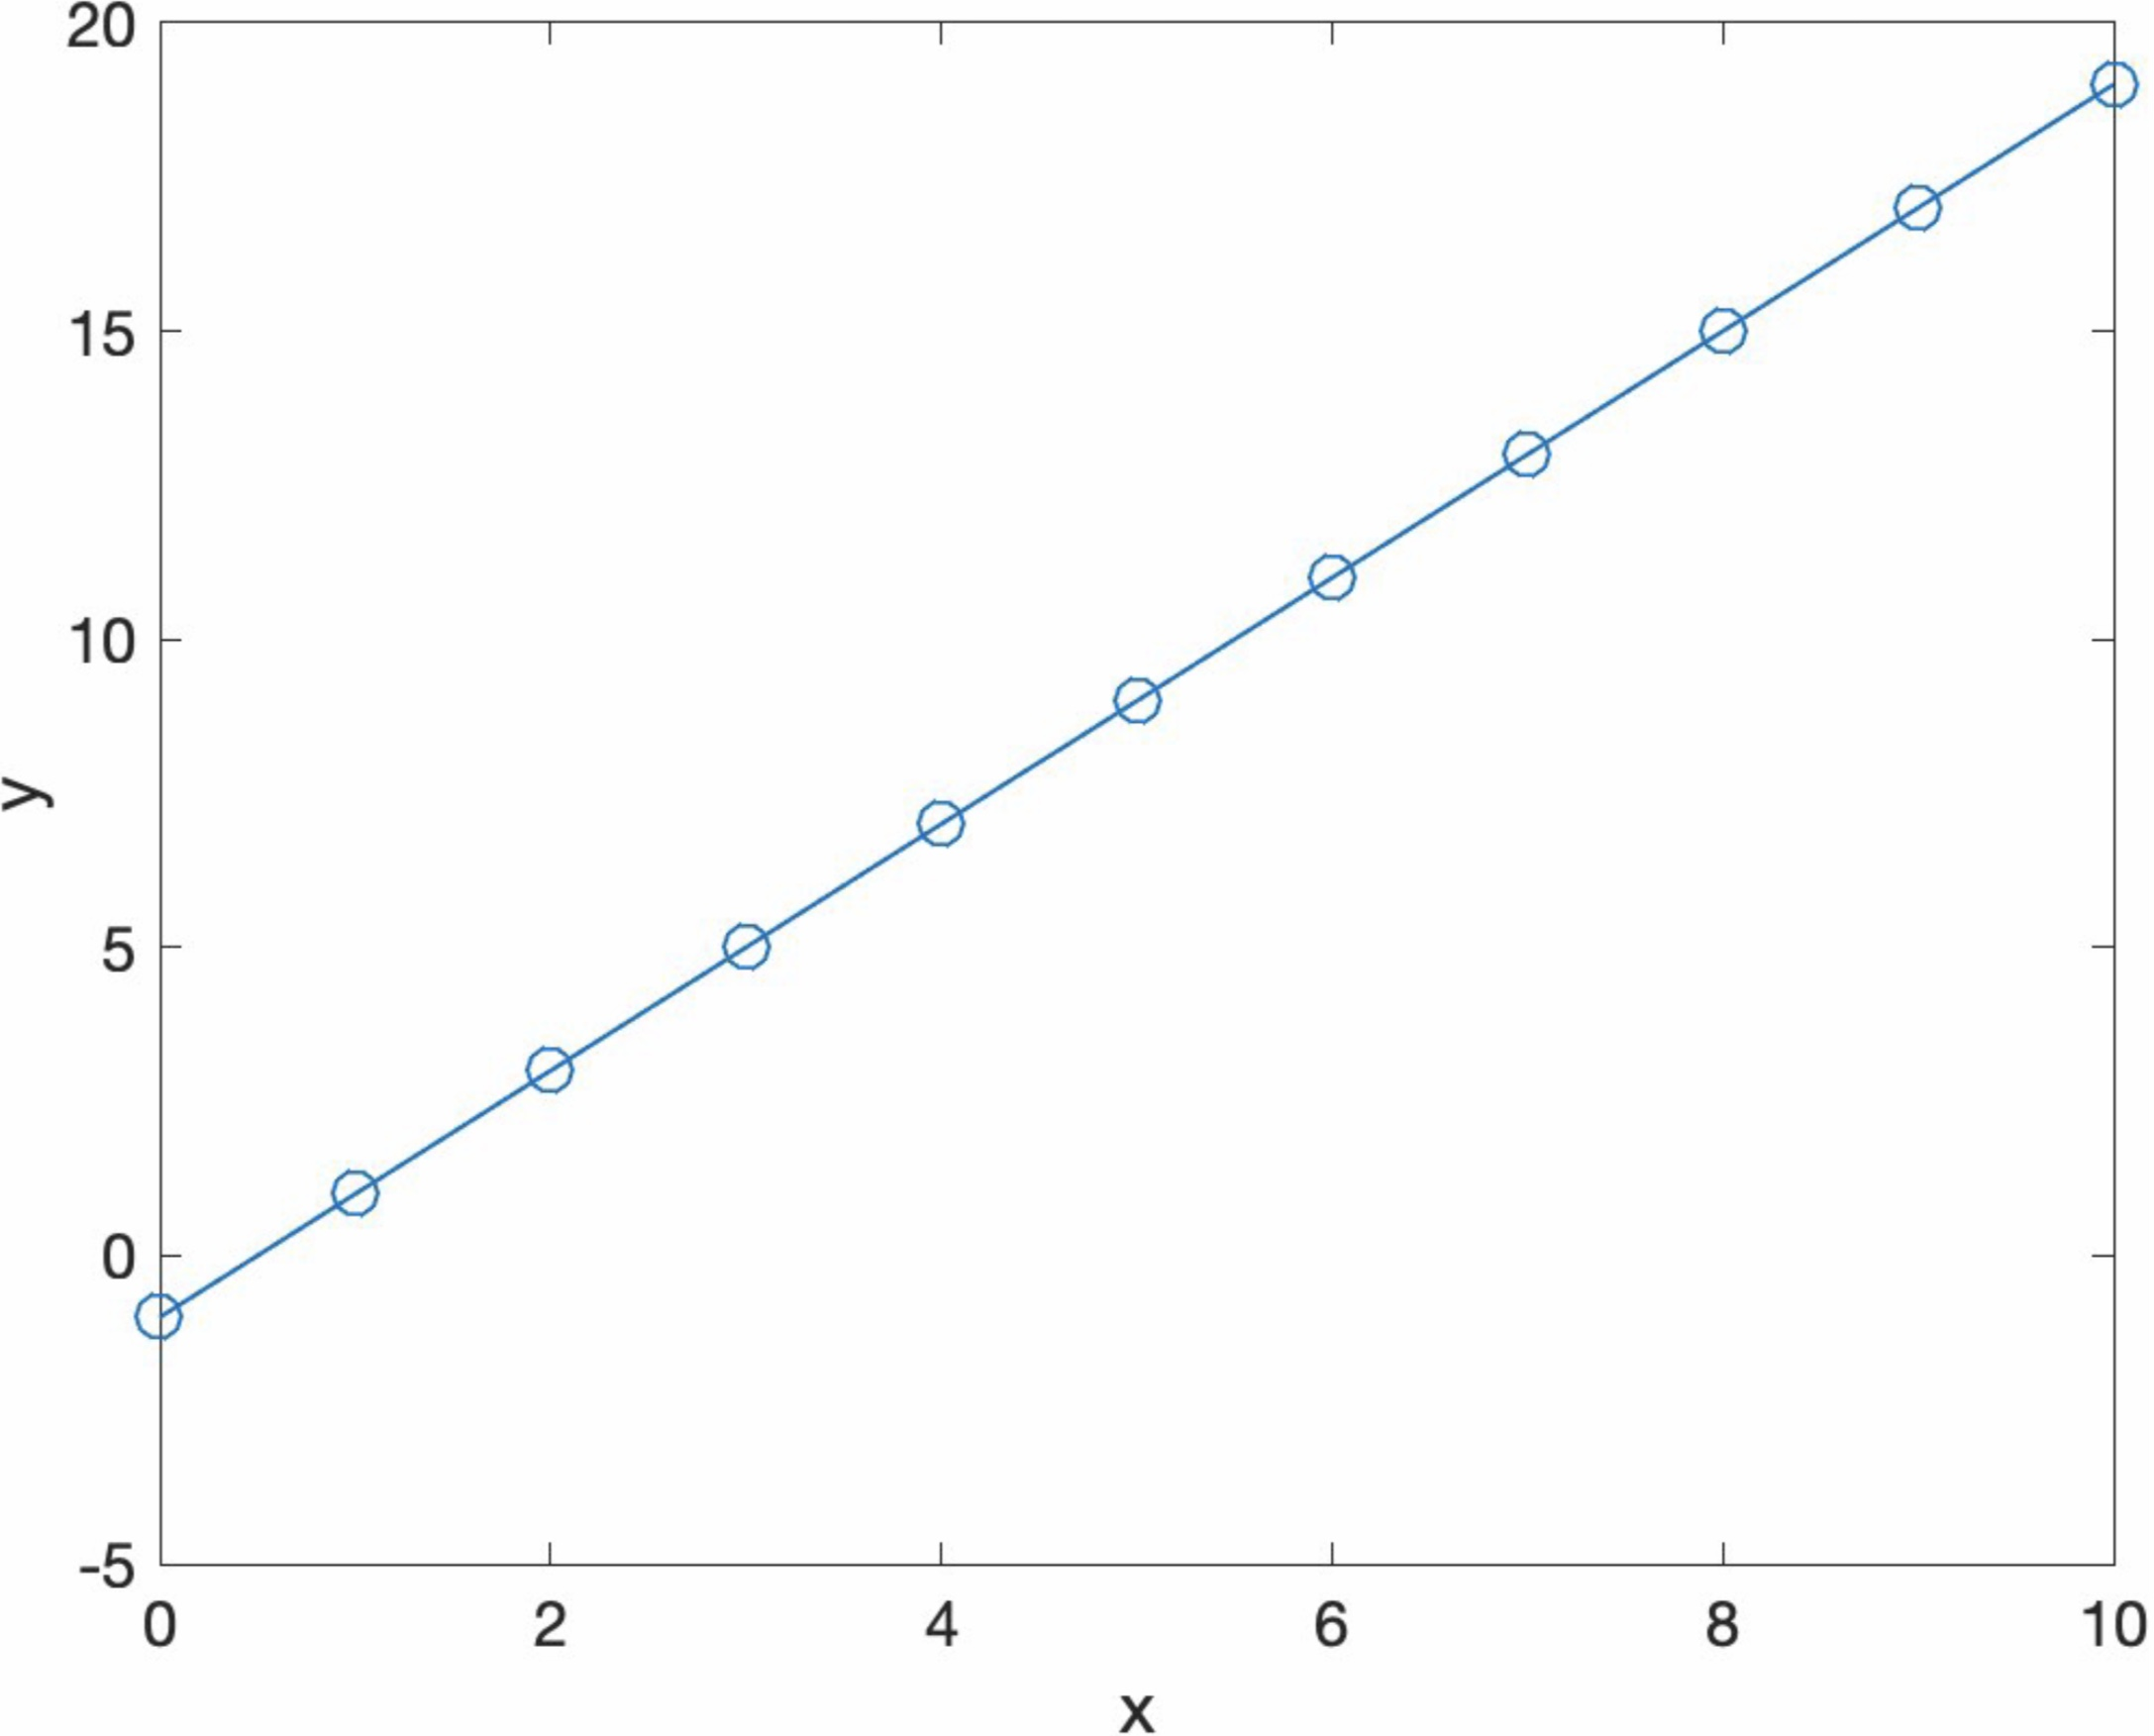
\includegraphics[width=0.5\textwidth]{immagini/4.10(1).jpg}
    \caption{Esempio di 10 dati esatti.}
    \label{fig:4.10(1)}
\end{figure}

Per la Figura \ref{fig:4.10(1)} è possibile affermare che la retta che passa per i 10 punti necessiterebbe solo di due punti per definirla e che i dati sono collineari. Se fossero interpolanti con una spline o con un polinomio interpolante sarebbe ottenuta una retta.

\begin{figure}
    \centering
    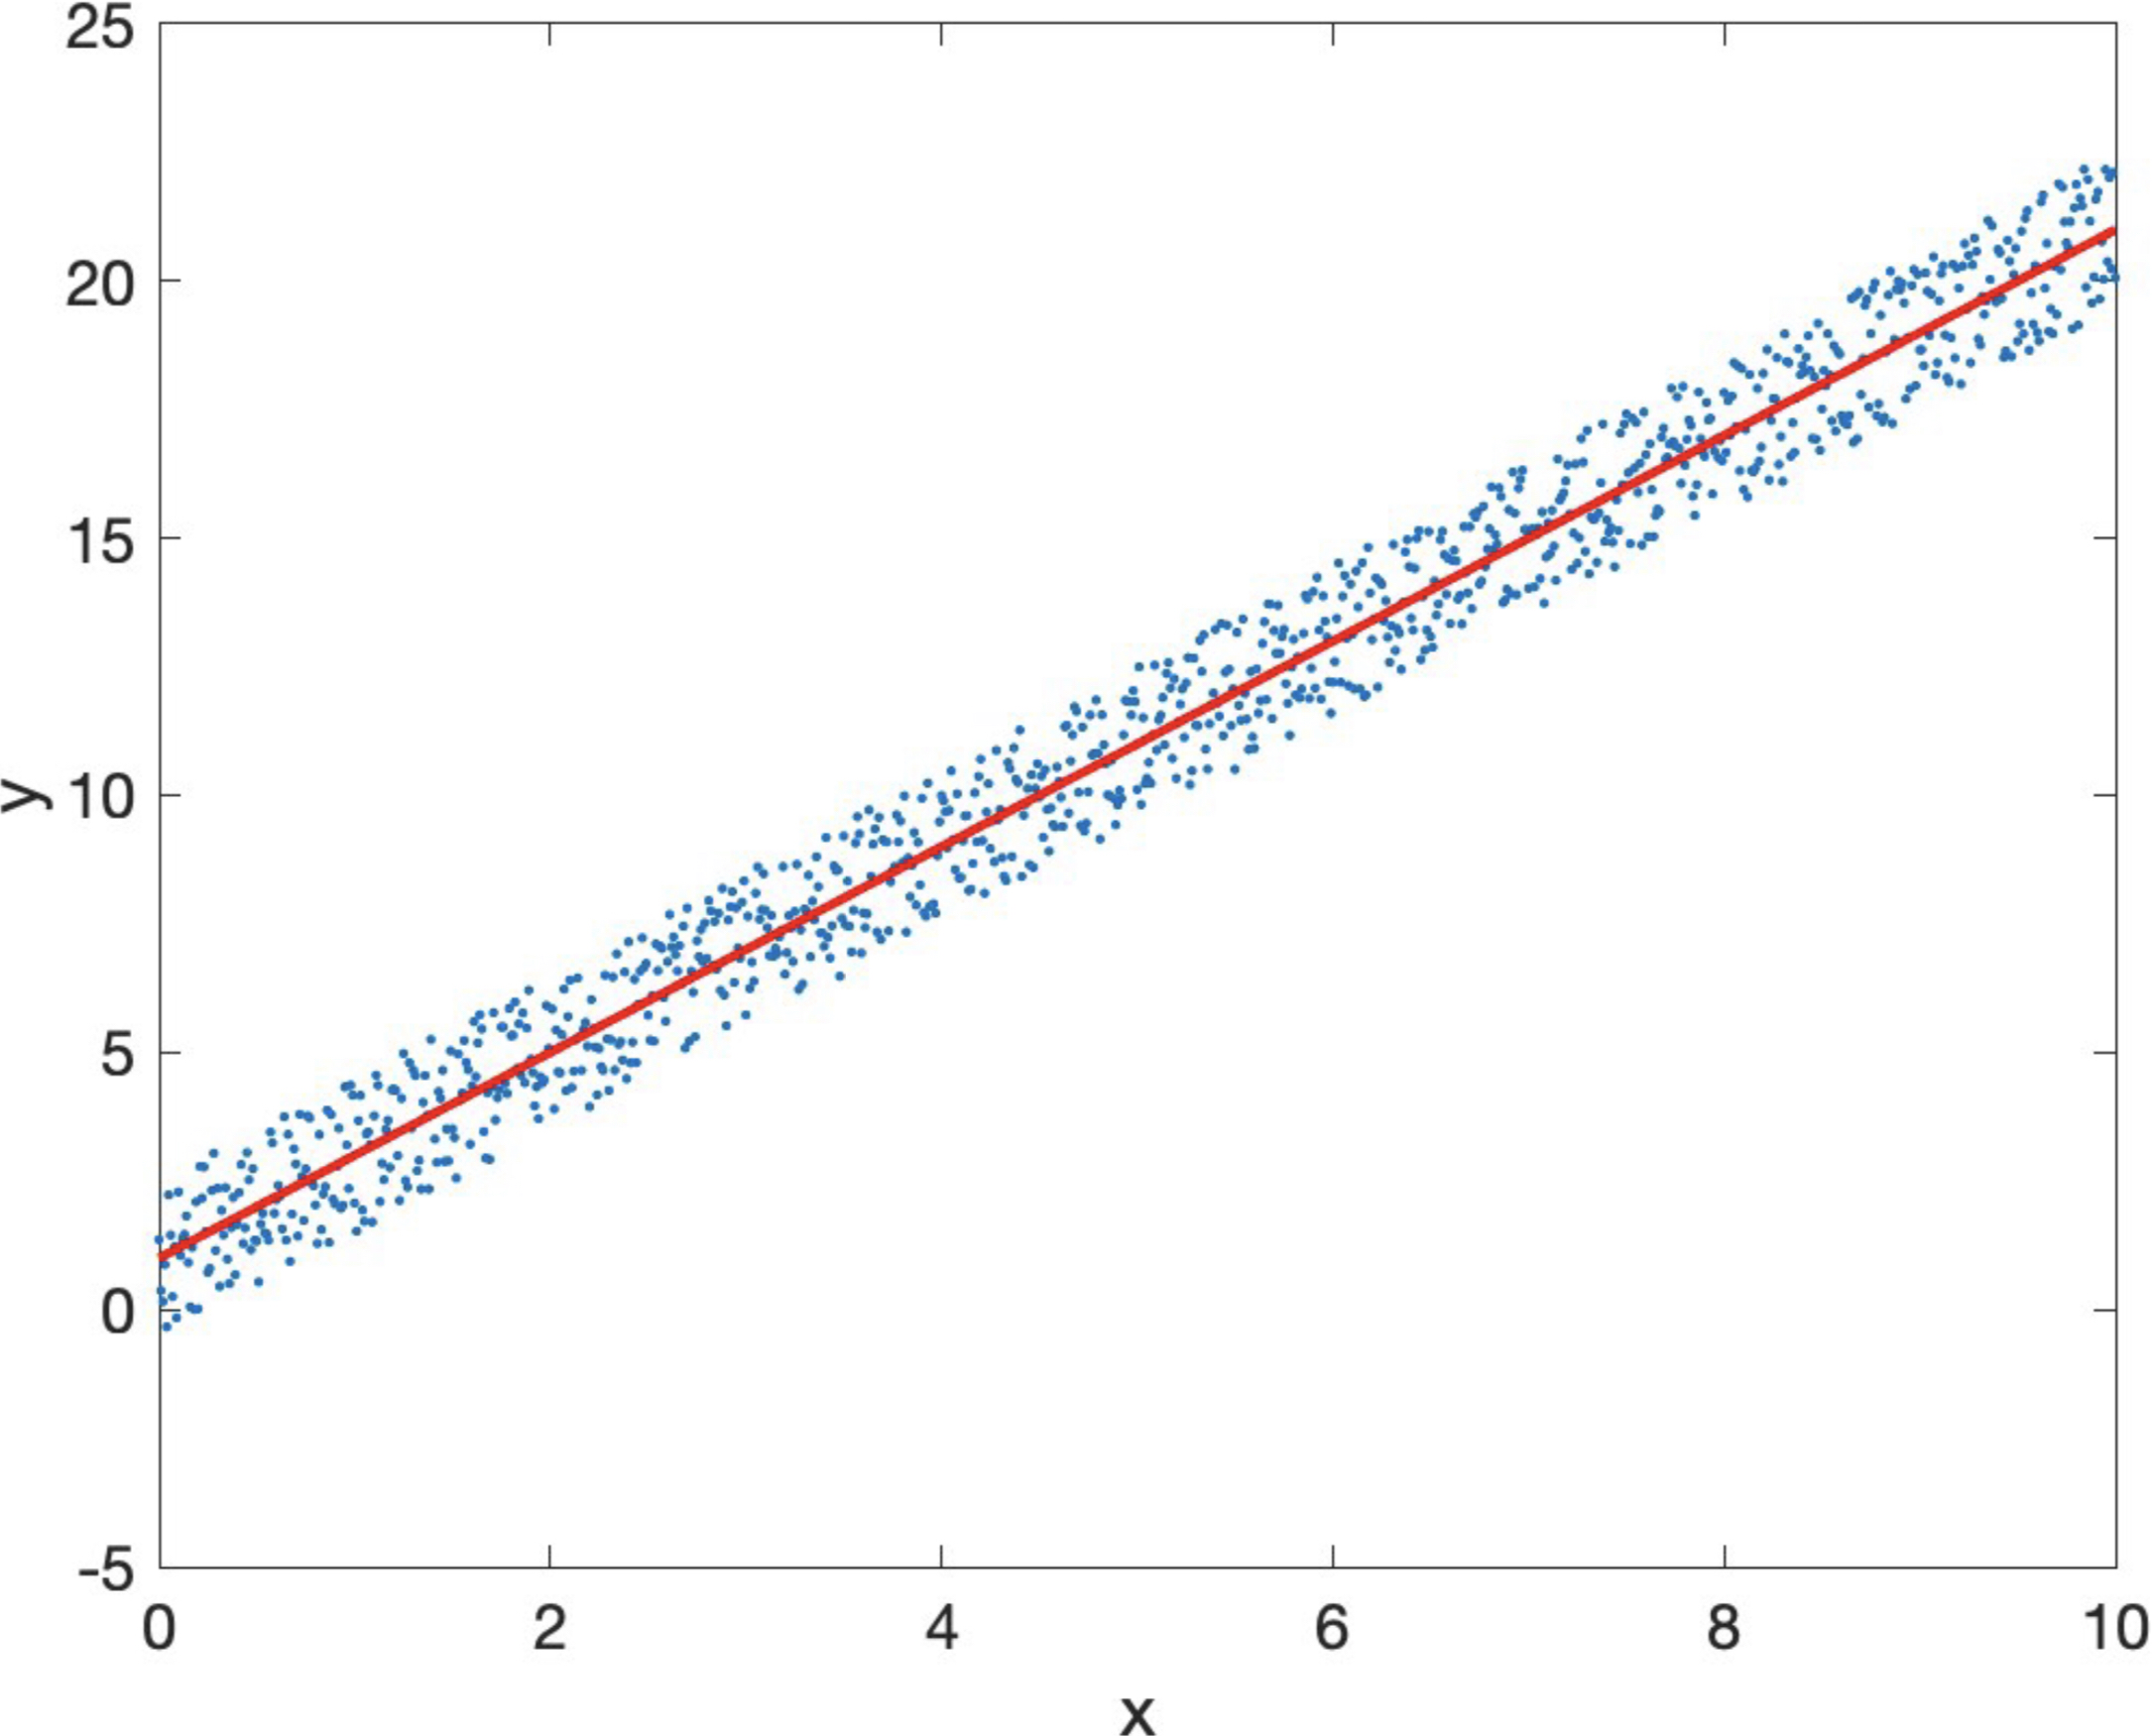
\includegraphics[width=0.5\textwidth]{immagini/4.10(2).png}
    \caption{Esempio di 1000 dati affetti da errore.}\label{fig:4.10(2)}
\end{figure}

Supposto di avere 1000 dati effetti da errore non sistematico, è ottenuta Figura \ref{fig:4.10(2)}. I dati, i puntini nella figura, sono ottenuti partendo dalla retta ed aggiungendo un termine d'errore, non lo stesso della retta, da un distribuzione gaussiana. Se fosse necessario interpolare allora il grafico oscillerebbe tra gli estremi dei puntini blu (più o meno periodicamente), non fornendo informazioni utili. La retta rossa, rappresentante la retta in Figura \ref{fig:4.10(1)}, approssima bene i dati.

\begin{figure}
    \centering
    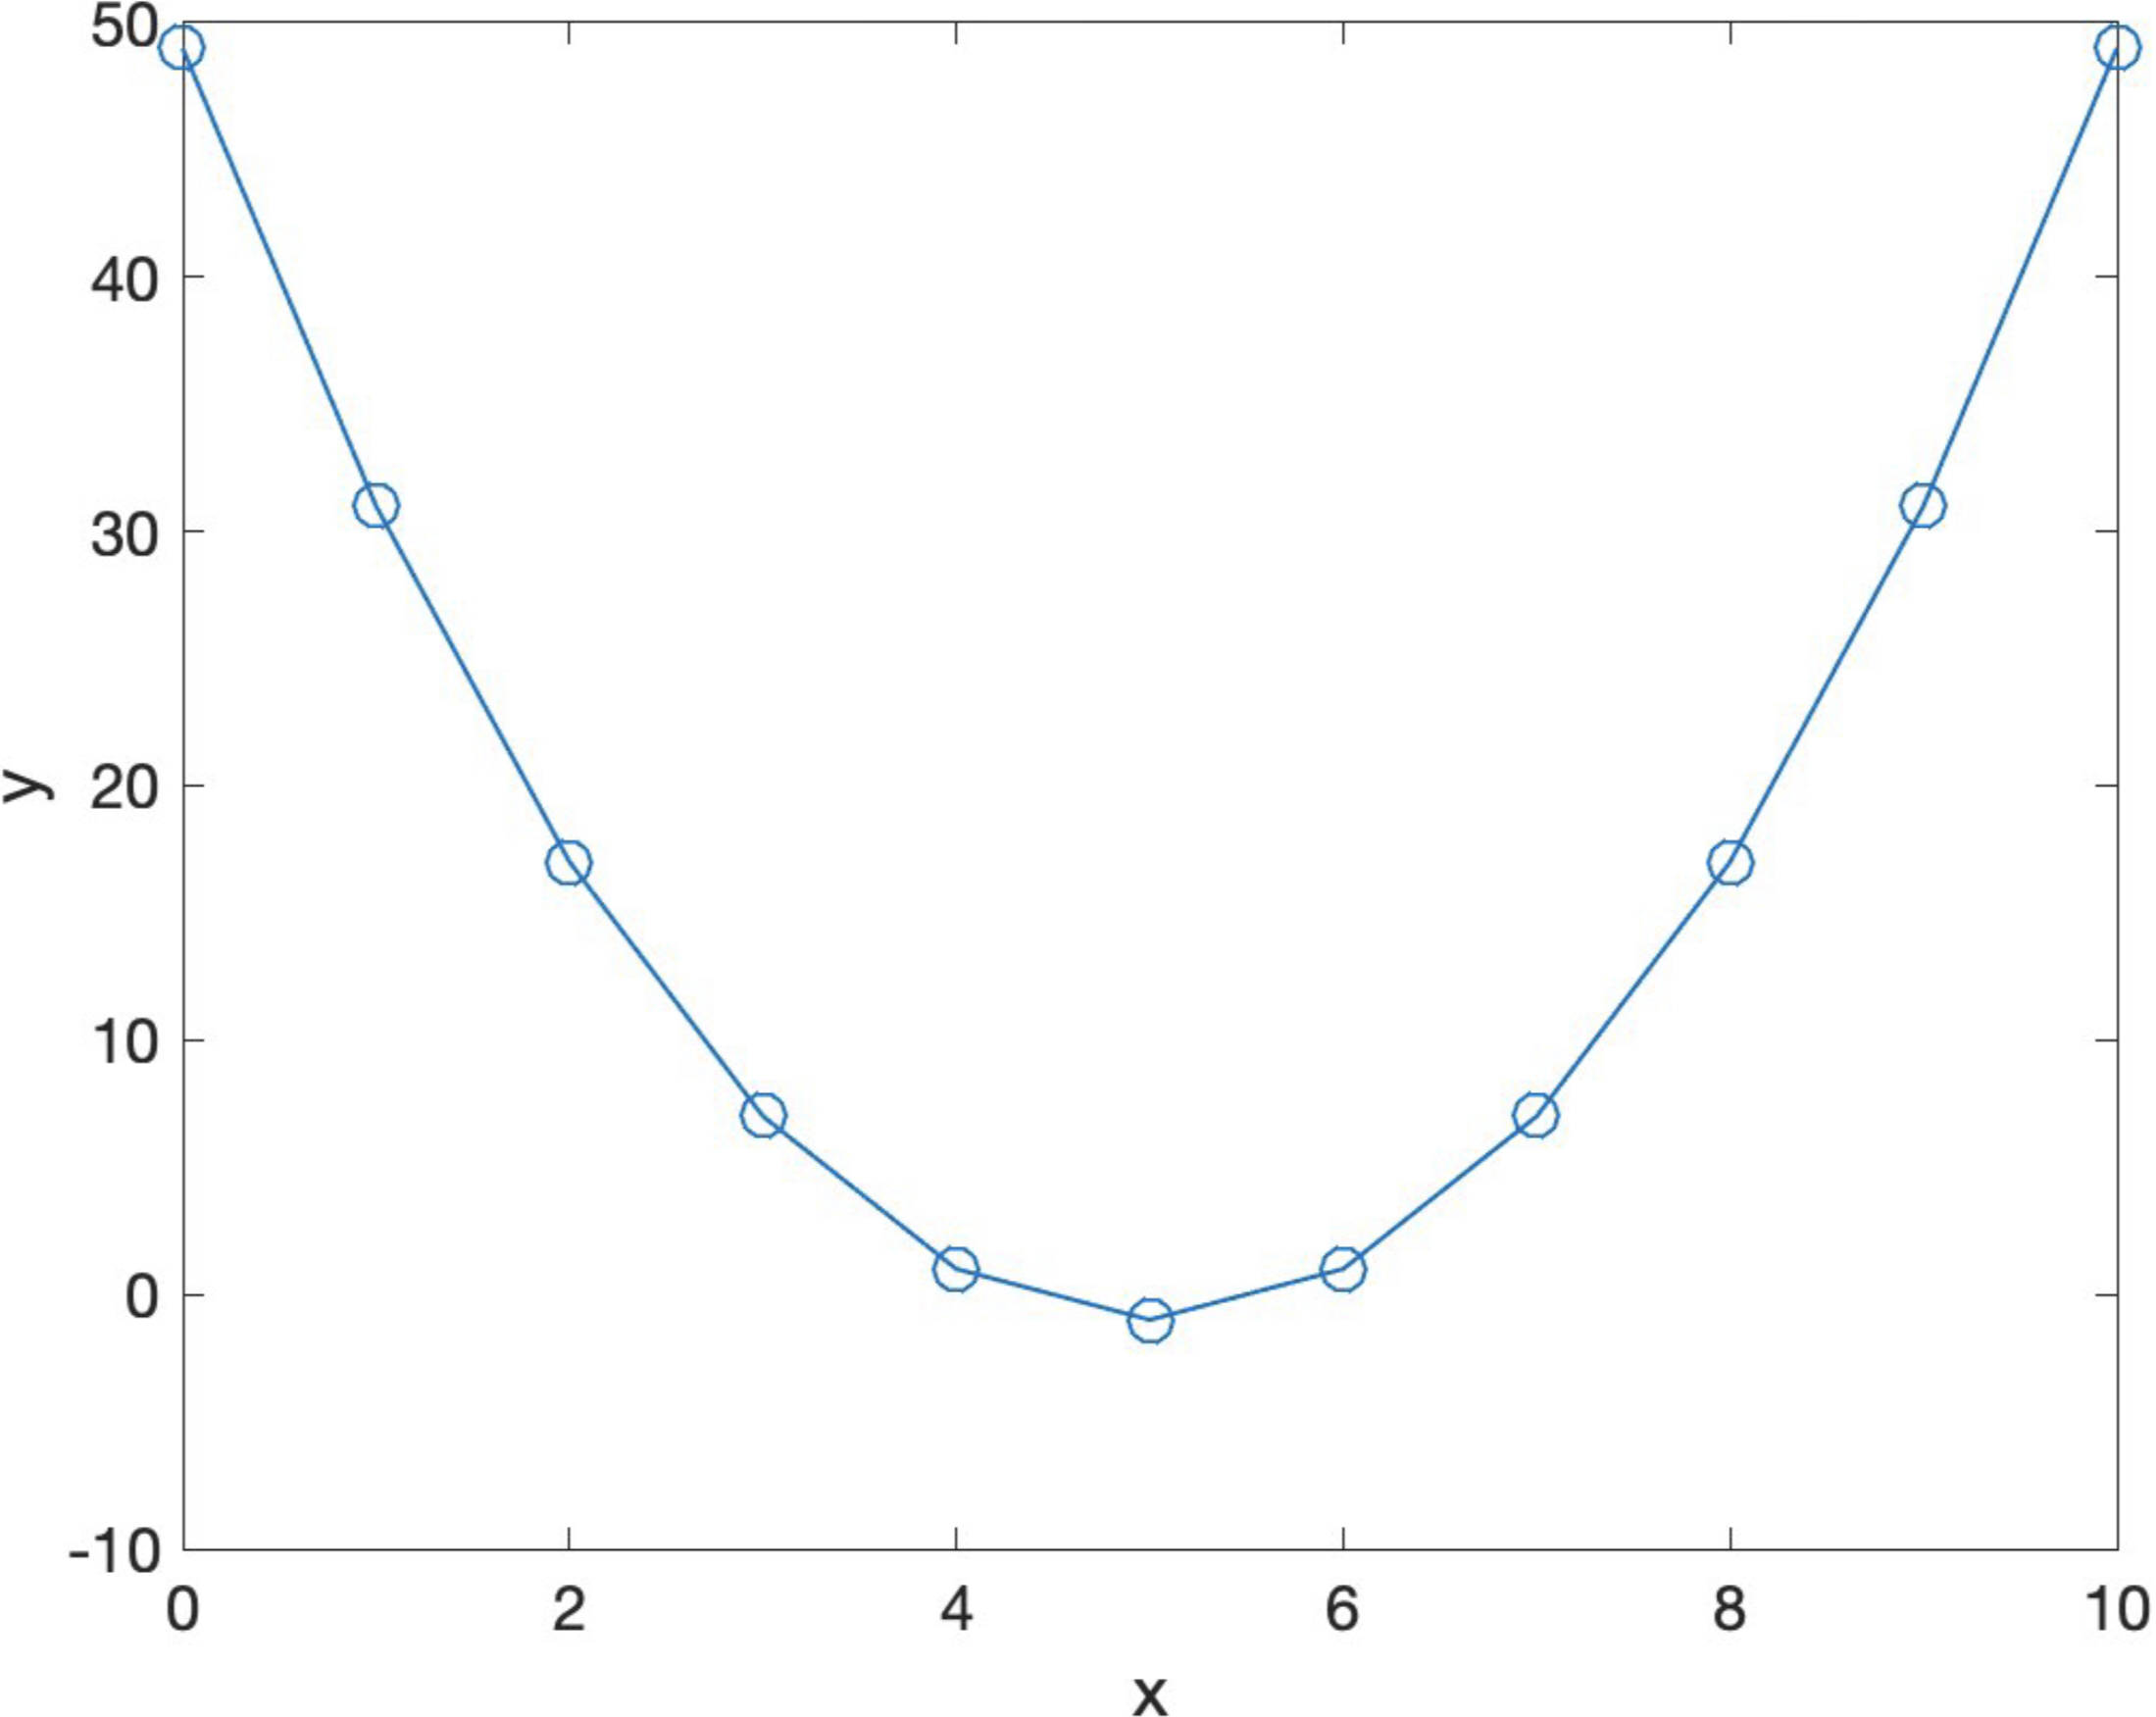
\includegraphics[width=0.5\textwidth]{immagini/4.10(3).png}
    \caption{Esempio di spline con $n=4$.}\label{fig:4.10(3)}
\end{figure}

\begin{figure}
    \centering
    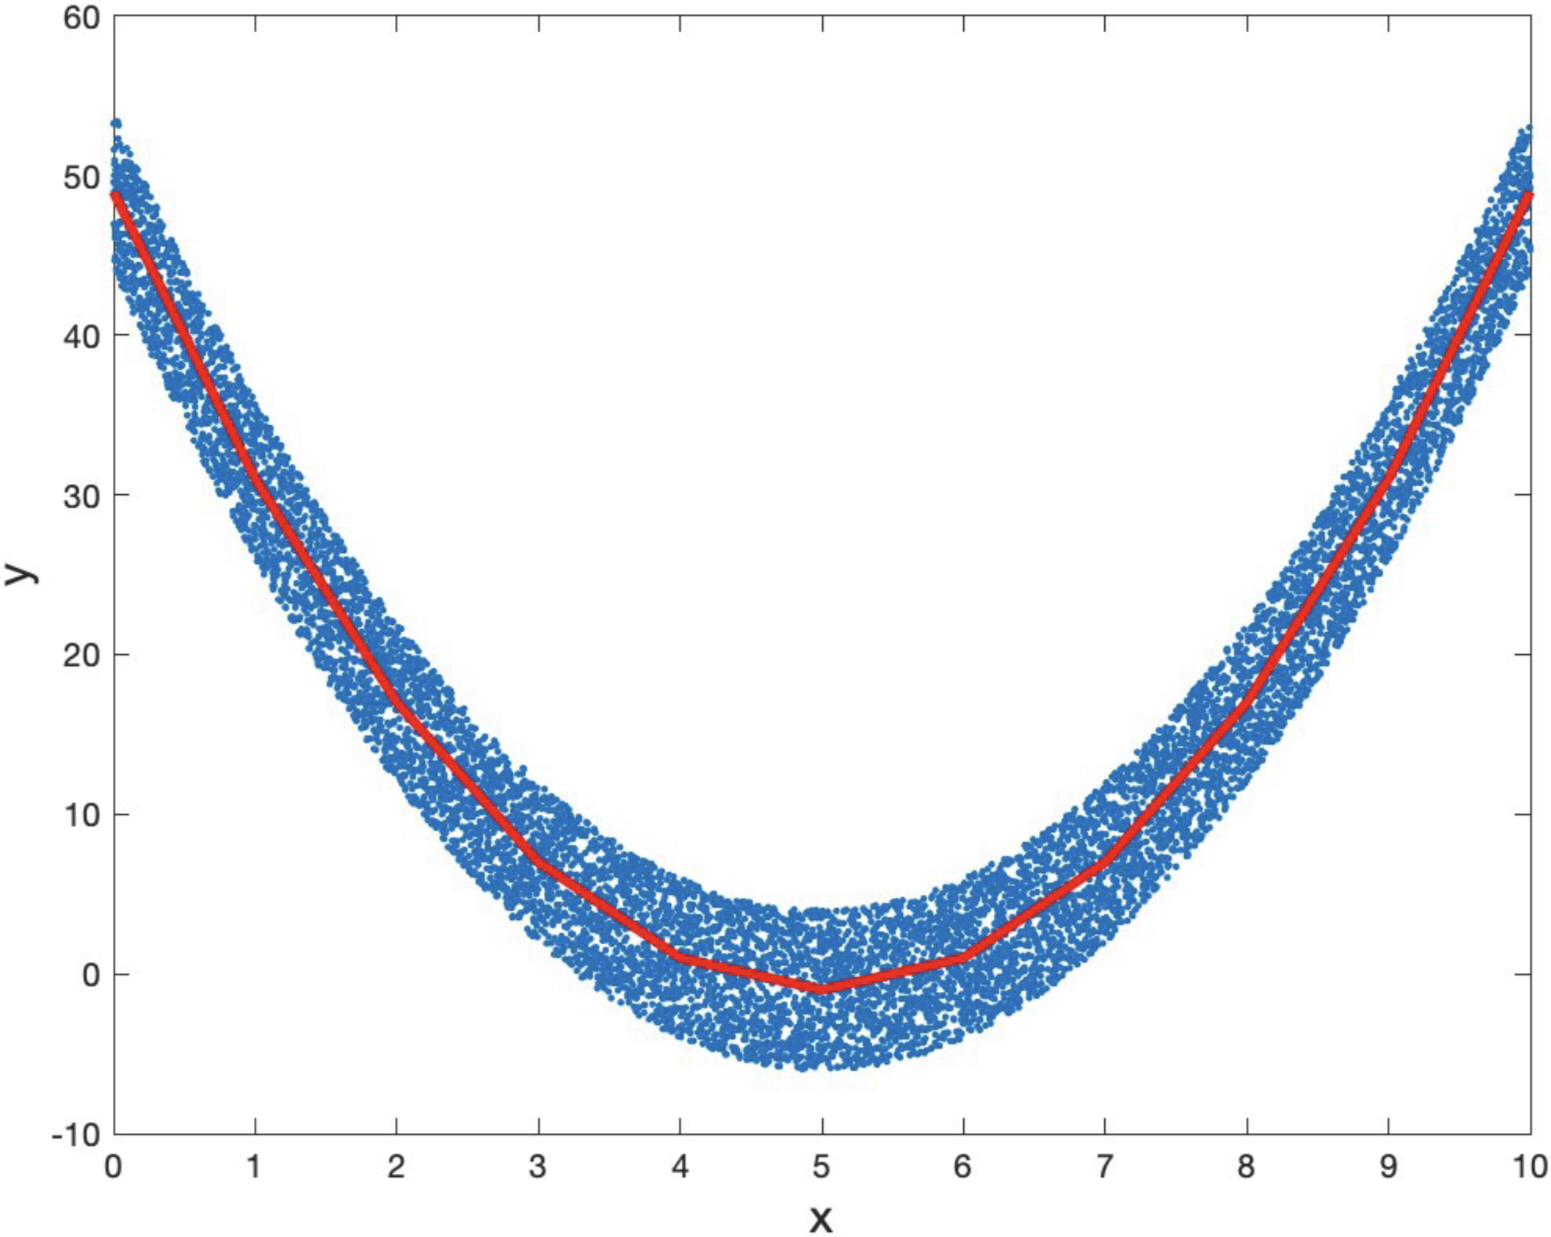
\includegraphics[width=0.5\textwidth]{immagini/4.10(4).png}
    \caption{Esempio di spline con 10000 dati.}\label{fig:4.10(4)}
\end{figure}

Per la Figura \ref{fig:4.10(4)} non ha senso calcolare il polinomio interpolante perché un polinomio di grado 10000 è impossibile da calcolare ed un polinomio si fatto non ha dati utili. Inoltre, la retta rossa della figura rappresenta la parabola di Figura \ref{fig:4.10(3)}, la quale approssima in modo soddifacente i dati.

Dalle Figure \ref{fig:4.10(1)}-\ref{fig:4.10(4)} è possibile affermare che è un caso che un punto utile sia trovato (perché sono troppi), infatti in genere non è trovato. 

Supposto di avere un fenomeno da rilevare, dipendente da un variabile indipendente $x$, che soddisfa una legge di tipo polinomiale (non inventata):
\begin{equation*}
    y=p(x),\quad p(x)\in\Pi_{\boldsymbol{m}}.
\end{equation*}

\begin{remark}
    In genere il grado $\boldsymbol m$ è noto a priori.
\end{remark}

Tuttavia, $y$, data l'uguaglianza sopra, è un polinomio del tipo
\begin{equation}\label{eq:polIgnMinQuad}
    p(x)=\sum_{k=0}^{m}a_kx^k,
\end{equation}
per il quale non sono noti i coefficienti del polinomio ma sono note le seguenti misurazioni del fenomeno:
\begin{equation}\label{eq:misFenMinQuad}
    \boldsymbol{(x_i,y_i),\quad i=1,\hdots,n,\quad n\geq m,\quad n}\overset{\footnotemark}{\boldsymbol{>>}}\boldsymbol{k+1}.
\end{equation}\footnotetext{$n$ è tipicamente molto maggiore di $k+1$, quindi il numero di misurazioni deve essere almeno pari al numero di coefficienti. Se $n=k+1$, ovvero $n$ è pari al numero di coefficienti, allora è calcolata l'interpolazione.}

\textbf{Il problema dell'approssimazione polinomiale nel senso dei minimi quadrati è determinare il polinomio (\ref{eq:polIgnMinQuad}), ovvero determinare i coefficienti} $\boldsymbol{a_0,\hdots, a_n}$\textbf{, che meglio approssima le coppie di dati definite come (\ref{eq:misFenMinQuad}).} Inoltre, è possibile osservare che il problema da risolvere è un sistema sovradimensionato ($n\geq m$).

\begin{remark}\label{re:ascDistPolm}
     È assunto che almeno $k+1$ delle ascisse $\{x_i\}$ siano distinte tra loro (dato $k$ il grado del polinomio da determinare)\footnote{Le $\{x_i\}$ possono essere utilizzate per effettuare più misurazioni in un punto in cui è necessario. È necessario che la condizione ($k+1$ ascisse distinte) sia soddisfatta per ammettere che la formulazione abbia soluzione unica.}.
\end{remark}

Per determinare i coefficienti incogniti del polinomio è necessario definire la migliore approssimazione dei dati. Il problema è rappresentato in forma vettoriale, quindi, dati i vettori
\begin{equation}
    \underline{y}=
    \begin{bmatrix}
        y_1\\
        \vdots\\
        y_n
    \end{bmatrix},\;
    \underline{z}=
    \begin{bmatrix}
        p(x_1)\\
        \vdots\\
        p(x_n)
    \end{bmatrix}
    \equiv
    \begin{bmatrix}
        \sum_{k=0}^m a_kx_1^k\\
        \vdots\\
        \sum_{k=0}^m a_kx_n^k
    \end{bmatrix},
\end{equation}
contenenti rispettivamente i valori attesi ed i valori misurati in corrispondenza delle ascisse $x_0,\hdots,x_n$, è determinato il vettore $a=(a_0,\hdots,a_m)^T$, il quale minimizza la norma $||r||_2^2=\sum_{k=0}^n|y_i-z_i|^2$ (ovvero la norma euclidea al quadrato del vettore residuo $\underline{r}=\underline{z}-\underline{y}$). Tuttavia, è possibile esprimere $\underline{z}$ come
\begin{equation*}
    \underline{z}\underset{\footnotemark}{=}
    \begin{bmatrix}
        x_1^0&\hdots &x_1^m\\
        &\vdots&\\
        x_n^0& \hdots &x_n^m
    \end{bmatrix}
    \begin{bmatrix}
        a_0\\
        \vdots\\
        a_m
    \end{bmatrix}
    \equiv V\underline{a},
\end{equation*}\footnotetext{La moltiplicazione riga di $V$ per a da la forma base di Lagrange.}con $V\in \mathbb R^{n\times k+1}$ matrice del tipo di Vandermonde. Quindi, ricercando il vettore $r$ di minima norma euclidea tale che $V\underline{a}=\underline{y}+\underline{r}$, il problema dell'approssimazione polinomiale si traduce nella ricerca della soluzione del sistema lineare sovradimensionato
\begin{equation}\label{eq:Va=y}
    V\underline{a}=\underline{y},
\end{equation}
nel senso dei minimi quadrati.

\begin{remark}
    \footnote{OSS 1 Slide 8 PDF 25.}
    $\overset{\footnotemark}{V\in\mathbb R^{n\times k+1}}$, con $n>k+1$. Questo significa che sono presenti più equazioni ($n$) che incognite ($k+1$).
\end{remark}\footnotetext{Sul libro, pagina 103, ha notazione diversa perché $n$ è indicizzato da 0, quindi è $n+1$.}

$\boldsymbol{V\underline{a}=\underline{y}}$ \textbf{è risolto tramite fattorizzazione $\boldsymbol{QR}$, sotto la condizione che la $\boldsymbol V$ abbia rango massimo ($\boldsymbol{m+1}$) affinché esista soluzione e questa sia unica.} Quindi, almeno $m+1$ delle ascisse $\{x_i\}$ devono essere distinte fra loro.

\begin{remark}
    \footnote{OSS 2 Slide 8 PDF 25, Teorema 4.12 PG 103.}
    La matrice $V$ ha rango massimo ($k+1$) sotto le ipotesi dell'Osservazione \ref{re:ascDistPolm}.
\end{remark}

Data $V$, del tipo di Vandermonde e le $k+1$ righe corrispondenti alle $k+1$ ascisse distinte, è ottenuta una matrice quadrata, la quale è una matrice di Vandermonde definita da ascisse distinte (quindi è nonsingolare). Se esiste una sottomatrice di dimensione $k+1$, ma singolare, questa ha rango massimo.

\paragraph{Fuori dalla lezione:} il vettore $\uline a$ in (\ref{eq:Va=y}) esiste ed è unico. Di conseguenza esiste ed è unico il polinomio di approssimazione ai minimi quadrati (\ref{eq:polIgnMinQuad}). Riguardo al costo computazionale per ottenere il polinomo di approssimazione ai minimi quadrati, è possibile affermare che valgono le stesse considerazioni riguardo alla fattorizzazione $QR$ fatte nelle Sezioni \ref{ssec:sistemi_lineari_sovradimensionati} e \ref{sssec:complHH}.

\begin{remark}
    \footnote{OSS 3 Slide 9 PDF 25} Pertanto, il problema è risolvibile utilizzando la fattorizzazione $V=QR$, con $Q\in\mathbb R^{n\times n}$ ortogonale e $R=\begin{pmatrix}\widehat R\\ 0\end{pmatrix}\in\mathbb R^{n\times k+1}$, dove $\widehat R\in\mathbb R^{(k+1)\times (k+1)}$, triangolare superiore e nonsingolare.
\end{remark}

\begin{remark}
    \footnote{OSS 4 Slide 8 PDF 25}
    Se $\boxed{n=k+1}$ è ottenuto il polinomio di grado $k$ che interpola $(x_i,y_i),\, i=0,\hdots,k$. 
\end{remark}

Per $n=k+1,\, V$ è quadrata ed ha rango massimo, quindi il sistema $V\uline a$ è risolvibile.

\begin{remark}
    \footnote{OSS 5 Slide 9 PDF 25, Osservazione 4.8 PG 104.} Questa tecnica di risoluzione è implementata nella funzione \textit{\textbf{polyfit}} di Matlab.
\end{remark}

\begin{remark}
    \footnote{OSS6 Slide 9 PDF 25.} Dato un sistema lineare quadrato
    \begin{equation}\label{eq:sistQuad}
        V\underline{a}=\underline{y}
    \end{equation}
    e $D$ una matrice nonsingolare, allora (\ref{eq:sistQuad}) ha la stessa soluzione di
    \begin{equation}\label{eq:sistQuadD}
        DV\underline{a}=D\underline{y}.
    \end{equation}
\end{remark}

$\overset{\footnotemark}{\text{Questo}}$ \textbf{non è più vero} se la matrice $D$ è $\overset{\footnotemark}{\text{rettangolare}}$ (perché (\ref{eq:sistQuad}) e (\ref{eq:sistQuadD}) non avrebbero più la solita soluzione). 

(\ref{eq:sistQuadD}) è utilizzato, nella pratica, calcolando $D=diag(\underline{p})$, con $\underline{p}$ vettore contenente una \textbf{distribuzione di probabilità discreta} ($\iff \underline{p}\geq 0 \,\land\, \text{sum}(\underline{p})=1$), per dare un diverso peso, $p_i$, a ciascuna equazione.

\addtocounter{footnote}{-1}
\footnotetext{È utilizzato "Questo" perché alcune volte, nella ricerca del polinomio che approssima i dati e che soddisfa nel senso dei minimi quadrati il sistema, alcuni dati sono più attendibili di altri. I dati sono pesati in base all'attendibilità, attraverso una distribuzione discreta sulle diagonali di $\underline{p}$, dove le righe corrispondenti a distribuzioni più grandi saranno più importanti di altre.}

\stepcounter{footnote}
\footnotetext{Ricavare la soluzione nel senso dei minimi quadrati del sistema lineare è diverso dal ricavare la soluzione nel senso dei minimi quadrati del sistema.}

\subsection{Risoluzione di un sistema tridiagonale}\label{ssec:risSistTridiag}

\noindent\footnote{Slide 8-10 PDF 23} È necessario, ai fini della Sezione \ref{ssec:calcSplineCub}, risolvere il sistema lineare
\begin{equation*}
    A\underline{x}=\underline{q}\in\mathbb{R}^n,
\end{equation*}

\noindent dove

\begin{equation*}
    A=
    \begin{bmatrix}
        a_1 & c_1 & & & &\\
        b_2 & a_2 & c_2 & & &\\
            & b_3 & a_3 & c_3 & &\\
            & & \ddots &\ddots & \ddots &\\
            & & & \ddots & \ddots & c_{n-1}\\
            & & & &  b_n & a_n
    \end{bmatrix}
    \in\mathbb{R}^{n\times n}
\end{equation*}
è una matrice triangolare. È supposto che questa sia fattorizzabile $LU$.

\begin{remark}\footnote{Slide 9 PDF 23.}
    È possibile \textbf{memorizzare $\boldsymbol A$ con 3 vettori (complessità lineare dei dati)}.
\end{remark}

%\hrule
%\vspace{4px}
\noindent Risolvere per fattori $LU$ ha complessità lineare. Invece di avere $\frac{2}{3}n^3$ flops per la fattorizzazione ed $n^2$ operazioni per i fattori triangolari. In questo caso la complessità è $n$ per la fattorizzazione ed $n$ per la risoluzione.

\noindent Errori da non fare: con complessità lineare è possibile risolvere problemi di qualsivoglia grandezza, con $n^2$ fino ad un certo punto e con ordine superiore al secondo no. Per risolvere il sistema tridiagonale alcune persone utilizzano una matrice piena, assegnano i tre vettori alle tre diagonali e le forniscono in input alla function di risoluzione, tramite fattorizzazione $LU$. In questo caso l'esercizio è valutato 0.
%\vspace{3px}
%\hrule
%\vspace{6px}

\noindent È necessario verificare $A$ che sia fattorizzabile $LU$, ovvero $\underset{\footnotemark}{A}=LU$, con
\footnotetext{$A$ è diagonale dominante quindi fattorizzabile $LU$.}
\begin{equation*}
    \begin{matrix}
        \underset{\footnotemark}{L}=
    \begin{bmatrix}
        1 & & & &\\
        l_2 & 1 & & &\\
        & l_3 & 1 & &\\
        & & \ddots & \ddots & &\\
        & & & l_n & 1
    \end{bmatrix}
    ,\; U\overset{\footnotemark}{=}
    \begin{bmatrix}
        d_1 & c_1 &\\
            & d_2 & c_2\\
            & & \ddots & \ddots\\
            & & & \ddots & c_{n-1}\\
            & & & & d_n
    \end{bmatrix},\\
    L\cdot U=
    \begin{bmatrix}
        d_1 & c_1 & & & &\\
        l_2d_1 & (d_2+l_2 c_1) & c_2 & & &\\
            & l_3d_2 & (d_3+l_3c_2) & c_3 & &\\
            & & \ddots &\ddots & \ddots &\\
            & & & \ddots & \ddots & c_{n-1}\\
            & & & &  l_nd_{n-1} & (d_n+l_nc_{n-1})
    \end{bmatrix}
    \end{matrix}
\end{equation*}
\addtocounter{footnote}{-1}
\footnotetext{Matrice biadiagonale memorizzabile con un vettore.}

\stepcounter{footnote}
\footnotetext{La diiagonale dei $d_i$ cambia rispetto ad A mentr la diagonale dei $c_i$ è uguale ad A.}

\noindent uguagliando gli elementi omologhi, ottenendo:\\
$d_1=a_1\\
\begin{rcases}
l_i=b_i/d_{i-1},\\
d_i=a_i-l_i\cdot c_{i-1},\; i=2,\hdots, n.
\end{rcases}$
al costo di $3n$ flops dove è possibile sovrascrivere $l_i\rightarrow b_i,\; d_i\rightarrow a_i$.

\noindent Il sistema bidiagonale per $L$ può essere risolto tramite l'utilizzo dell'Algoritmo \ref{alg:calcSistBdiagL}, con $\underline{x}\leftarrow\underline{q}$.

\begin{algorithm}\caption{Algoritmo risoluzione sistema bidiagonale per $L$}
\label{alg:calcSistBdiagL}
    \begin{lstlisting}[style=Matlab-editor]
    for i = 2 : n
        x_i = x_i - e_i x_(i - 1) % (2n flops)
    end
    \end{lstlisting}
\end{algorithm}

\noindent Il sistema bidiagonale per $U$ può essere risolto con l'Algoritmo \ref{alg:calcSistBdiagU}.
\begin{algorithm}\caption{Algoritmo risoluzione sistema bidiagonale per $U$}
\label{alg:calcSistBdiagU}
    \begin{lstlisting}[style=Matlab-editor]
    x_n = x_n / d_n
    for i = n - 1 : -1 : 1
            x_i = (x_i - c_i x_(i + 1)) / d_i %(3n flops)
    end
    \end{lstlisting}
\end{algorithm}

\noindent Quindi al posto di $\frac{2}{3}n^3$ flops c'è $3n$ ed al posto di $n^2\; 2n$. Totale $8n$ flops, mentre se è simmestrica $7$ flops.

\noindent Morale: se è richiesto di risolvere un sistema tridiagonale fattorizzabile $LU$ allora è necessario utilizzare l'Algoritmo \ref{alg:calcSistBdiagU}, non assegnando i 3 vettori ad una matrice e richiamando la function per la risoluzione fattorizzabile $LU$.